%%%%%%%%%%%%%%%%%%%%%%%%%%%%%%%%%%%%%%%%%%%%%%%%%%%%%%%%%%%%%%%%%%%%
%% I, the copyright holder of this work, release this work into the
%% public domain. This applies worldwide. In some countries this may
%% not be legally possible; if so: I grant anyone the right to use
%% this work for any purpose, without any conditions, unless such
%% conditions are required by law.
%%%%%%%%%%%%%%%%%%%%%%%%%%%%%%%%%%%%%%%%%%%%%%%%%%%%%%%%%%%%%%%%%%%%

\documentclass[
  printed, %% This option enables the default options for the
           %% digital version of a document. Replace with `printed`
           %% to enable the default options for the printed version
           %% of a document.
  oneside, %% This option enables double-sided typesetting. Use at
           %% least 120 g/m² paper to prevent show-through. Replace
           %% with `oneside` to use one-sided typesetting; use only
           %% if you don’t have access to a double-sided printer,
           %% or if one-sided typesetting is a formal requirement
           %% at your faculty.
  notable,   %% This option causes the coloring of tables. Replace
           %% with `notable` to restore plain LaTeX tables.
  nolof,     %% This option prints the List of Figures. Replace with
           %% `nolof` to hide the List of Figures.
  nolot,     %% This option prints the List of Tables. Replace with
           %% `nolot` to hide the List of Tables.
  %% More options are listed in the user guide at
  %% <http://mirrors.ctan.org/macros/latex/contrib/fithesis/guide/mu/fi.pdf>.
]{fithesis3}
\usepackage{gensymb}
\usepackage{subcaption}
%% The following section sets up the locales used in the thesis.
\usepackage[resetfonts]{cmap} %% We need to load the T2A font encoding
\usepackage[T1,T2A]{fontenc}  %% to use the Cyrillic fonts with Russian texts.
\usepackage[
  main=slovak, %% By using `czech` or `slovak` as the main locale
                %% instead of `english`, you can typeset the thesis
                %% in either Czech or Slovak, respectively.
  english, german, russian, czech, slovak %% The additional keys allow
]{babel}        %% foreign texts to be typeset as follows:
%%
%%   \begin{otherlanguage}{german}  ... \end{otherlanguage}
%%   \begin{otherlanguage}{russian} ... \end{otherlanguage}
%%   \begin{otherlanguage}{czech}   ... \end{otherlanguage}
%%   \begin{otherlanguage}{slovak}  ... \end{otherlanguage}
%%
%% For non-Latin scripts, it may be necessary to load additional
%% fonts:
\usepackage{paratype}
\def\textrussian#1{{\usefont{T2A}{PTSerif-TLF}{m}{rm}#1}}
%%
%% The following section sets up the metadata of the thesis.
\thesissetup{
    date          = \the\year/\the\month/\the\day,
    university    = mu,
    faculty       = fi,
    type          = bc,
    author        = Henrieta Micheľová,
    gender        = f,
    advisor       = {prof. RNDr. Ivana Černá, CSc.},
    title         = {Distribuované algoritmy pro rekonfiguraci platformy RoFI},
    TeXtitle      = {Distribuované algoritmy pro rekonfiguraci platformy RoFI},
    keywords      = {modulárny, robot, RoFIbot, distribuovaný algoritmus, rekonfigurácia, platforma RoFI, MPI, OpenMPI},
    TeXkeywords   = {modulárny, robot, RoFIbot, distribuovaný algoritmus, rekonfigurácia, platforma RoFI, MPI, OpenMPI},
    abstract      = {Platforma RoFI je nová modulárna robotická platforma vyvíjaná v~laboratóriu ParaDiSe. Táto práca stavia na už definovaných konceptoch platformy a prináša nový pohľad na rekonfiguráciu modulárnych robotov tejto platformy. Ďalej navrhuje a implementuje riešenie problému rekonfigurácie robotov z~distribuovaného hľadiska, teda z~pohľadu jedného modulu. Prínosom tejto práce je nástroj \textit{rofi-distribute}, ktorý poskytuje dva algoritmy na výpočet distribuovanej rekonfigurácie, ktoré boli otestované na sade príkladov. Výsledkami práce sú tiež porovnania navrhnutých algoritmov medzi sebou navzájom, ale aj porovnanie voči existujúcemu riešeniu problému rekonfigurácie z~pohľadu dĺžky trvanie výpočtov a počtu krokov rekonfigurácie. },
    thanks        = {Veľká vďaka patrí všetkým ľudom v~laboratóriu ParaDiSe za príjemnú atmosféru pri práci a každodennú čokoládu, hlavne celému tímu, ktorý sa podieľa na vývoji platformy RoFI, a to menovite vedúcej práce Ivane Černej a ďalším členom: Jiřímu Barnatovi, Janovi Mrázkovi, Viktórii Vozárovej a Markéte Naušovej, ktorí boli vždy ochotní zodpovedať mi otázky, prípadne konzultovať nápady. 
    
    Rovnaká vďaka patrí aj Vladimírovi Štillovi za pohotovú pomoc pri technických komplikáciách a Lukášovi Korenčikovi za podporu pri práci počas sviatkov a víkendov. Ďalej aj Tomášovi Szaniszlovi za podporu a korekcie textu práce do neskorých nočných hodín. V~neposlednom rade rodine a kamarátom za ich podporu nielen pri tvorbe tejto práce. },
    bib           = bibliography.bib,
}
\usepackage{makeidx}      %% The `makeidx` package contains
\makeindex                %% helper commands for index typesetting.
%% These additional packages are used within the document:
\usepackage{paralist} %% Compact list environments
\usepackage{amsmath}  %% Mathematics
\usepackage{amsthm}
\usepackage{amsfonts}
\usepackage{url}      %% Hyperlinks
\usepackage{markdown} %% Lightweight markup
\usepackage{listings} %% Source code highlighting
\lstset{
  basicstyle      = \ttfamily,%
  identifierstyle = \color{black},%
  keywordstyle    = \color{blue},%
  keywordstyle    = {[2]\color{cyan}},%
  keywordstyle    = {[3]\color{olive}},%
  stringstyle     = \color{teal},%
  commentstyle    = \itshape\color{magenta}}
  
\usepackage{multirow}
\usepackage{lscape}
\usepackage{longtable}
%\usepackage{floatrow} %% Putting captions above tables
%\floatsetup[table]{capposition=top}

\usepackage{enumitem}
\setitemize{itemsep=-5pt,topsep=10pt,parsep=10pt,partopsep=10pt}
\setenumerate{itemsep=-5pt,topsep=10pt,parsep=10pt,partopsep=10pt}
\usepackage[slovak,linesnumbered,ruled,vlined]{algorithm2e}
\newtheorem{lemma}{Lema}
\usepackage{minted}

\usepackage{color}
\definecolor{modra}{rgb}{0,0,1}
\definecolor{zlta}{rgb}{1,1,0}
\definecolor{cervena}{rgb}{1,.2706,.2667}

\definecolor{table-green}{rgb}{.588,1,.471}
\definecolor{table-red}{rgb}{1,.5,.5}

\usepackage[table]{xcolor}
    
\begin{document}
\chapter*{Úvod}
\addcontentsline{toc}{chapter}{Úvod}
V~súčasnej dobe sa vývoj robotických systémov presúva z~jednoúčelových strojov na univerzálne modulárne roboty. Hlavnými výhodami modulárnej robotiky je ich univerzálnosť a rekonfigurovateľnosť (či už manuálna alebo automatizovaná) \cite{modularAdvantage}. Táto voľnosť v~ich využívaní však otvára mnohé problémy, ktoré jednoúčelové roboty neriešia. 

Táto práca je zameraná na riešenie jedného z~najväčších problémov modulárnych robotov, a to ich schopnosti rekonfigurovať sa, v~kontexte novovznikajúcej robotickej platformy RoFI \cite{rofiWeb}. 

V~prvej časti práce sa nachádza popis fyzických komponentov spomenutej platformy, ktoré sa aktívne podieľajú na rekonfigurácii. Ide hlavne o~\textit{univerzálny modul} (ďalej už iba modul), ktorý je základnou stavebnou jednotku väčšiny modulárnych robotických platforiem. 

Ďalej nasleduje predstavenie matematického modelu, ktorý reprezentuje popísaný fyzický modul, a zároveň aj robotov, ktorí vzniknú spojením modulov. Tento model je prevzatý z~diplomovej práce \textit{Motion Planning for the RoFI Platform} \cite{vozarovaMasterThesis}, ale je upravený pre potreby algoritmov, ktoré sú v~tejto práci navrhnuté a implementované. 

Po popise matematického modelu nasleduje popis samotných rekonfiguračných algoritmov. Táto práca obsahuje dva návrhy riešenia problému rekonfigurácie modulárnych robotov, pričom oba z~nich využívajú vlastnosť, že robot vytvorený z~modulov je distribuovaný systém. 

Ďalšou časťou práce je samotná implementácia, ktorá rozširuje knižnicu RoFILib. Práca taktiež zahŕňa popis využitia časti spomenutej knižnice, ktorá bola implementovaná ako súčasť tejto práce. 

Navrhnuté a implementované algoritmy sú následne v~práci aj evaluované na sade vstupných príkladov konfigurácií. Evaluácia sa skladá z~porovnania oboch algoritmov z~pohľadu dĺžky trvania výpočtu rekonfigurácie a dĺžky rekonfiguračnej postupnosti. Zároveň je v~nej zaradené aj porovnanie s~algoritmom \textit{A*} navrhnutom a implementovanom vo vyššie spomínanej diplomovej práci. 

V~závere práce sa nachádzajú návrhy ako je možné zlepšiť obidva navrhnuté algoritmy. 

% ------------------------------------------------------ 1 ------------------------------------------------------
\chapter{Popis platformy RoFI}
\label{sec:platform}
RoFI je modulárna robotická platforma, ktorá vzniká na pôde Fakulty informatiky Masarykovej univerzity v~laboratóriu ParaDiSe\footnote{skratka pre Laboratoř paralelních a distribuovaných systémů (webstránka laboratória: \url{https://paradise.fi.muni.cz/})}. Táto platforma zastrešuje vývoj modulárnych robotov a iného príslušenstva po ich hardvérovej, ale aj softvérovej stránke. 

Primárnym cieľom platformy RoFI je vytvorenie modulárnych robotov, ktoré je možné využiť na rôzne úlohy. Príkladom sú úlohy ako prechádzanie cez úzke priestory, prekonávanie prekážok a podobne. 

Ich dizajn je navrhovaný tak, aby bolo jednoduché a nie príliš finančne náročné ich fyzicky skonštruovať. Softvérové vybavenie pokrýva široké spektrum požiadaviek modulárnych robotov a má jednoduché použitie pre používateľov s~rôznou úrovňou znalostí. 

Platforma je navrhnutá tak, aby bola ľahko rozšíriteľná o~dodatočné periférie a pasívne prvky. Celý vývoj prebieha ako open-source projekt \cite{rofiGit}. 

Základnou jednotkou platformy RoFI sú \textit{moduly} \cite{mrazekMasterThesis}, ktoré sú schopné sa vzájomne fyzicky prepojiť a zároveň medzi sebou komunikovať \cite{rofiCom}. Okrem toho sa každý modul dokáže pripojiť aj na pasívne prvky. 

Prepojenie viacerých modulov umožňuje vytvoriť tzv. \textit{RoFIbotov} \cite{rofiWeb}, ktoré majú širšie spektrum funkcionalít ako samostatné moduly. Cieľom tejto práce je práve zamerať sa na RoFIbotov a ich schopnosť rekonfigurovať sa za špecifických podmienok. 

Pre účely tejto práce je popísaná iba časť hardvérového vybavenia modulu a schopnosti prepájania modulov. Ďalšie rozšírenia, softvérové vybavenie a iné komponenty a návody sa nachádzajú na stránkach platformy \cite{rofiWeb}.

\section{Popis modulu}
\label{sec:moduleSpec}
RoFIbota je možné umiestniť do 3D siete tak, že každý modul sa nachádza v~práve dvoch políčkach siete (tzv. \textit{lattice type}). Toto rozdelenie je navrhnuté tak, že každá z~jeho dvoch strán (side) sa nachádza v~práve jednom políčku (popis tvaru modulu sa nachádza nižšie). 

Toto umiestnenie do 3D mriežky má tú výhodu, že tvar modulu je prispôsobený tak, aby pri pohybe zasahoval do najnižšieho možného počtu políčok siete (tzv. \textit{grid-awareness} \cite{mrazekMasterThesis}). 

V~súčasnej dobe je platforma RoFI prispôsobená na mriežku s~veľkosťou $10$\,cm. Podrobný popis vlastností modulu sa nachádza v~diplomovej práci \textit{RoFI – Distributed Metamorphic Robots} \cite{mrazekMasterThesis}. 

\begin{figure}[hbt!]
    \centering
    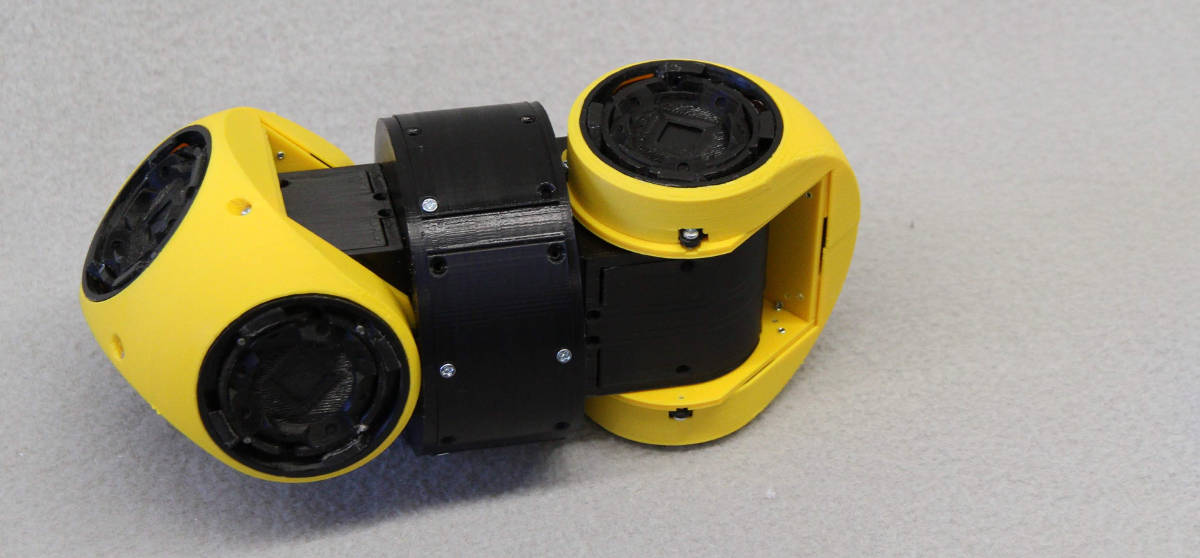
\includegraphics[width=0.6\textwidth]{pictures/module.jpg}
    \caption[Fotografia modulu]{Fotografia modulu \cite{rofiWeb}.}
    \label{fig:module}
\end{figure}

Každý z~modulov sa skladá zo \textit{strany A} (\textit{side A}) a \textit{strany B} (\textit{side B}). Každá z~nich sa delí na dve časti označené ako \textit{telo} (\textit{body}) a \textit{topánka} (\textit{shoe}) (viď obrázok \ref{fig:module_parts}). 

\begin{figure}[hbt!]
    \centering
    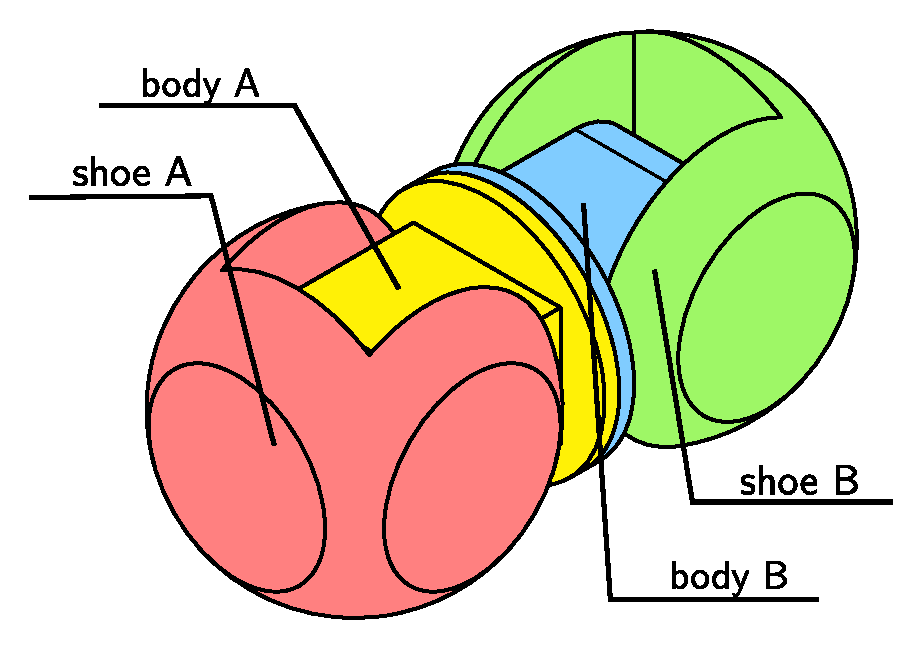
\includegraphics[width=0.6\textwidth]{pictures/module_parts.pdf}
    \caption[Časti modulu]{Schéma častí modulu \cite{mrazekMasterThesis}.}
    \label{fig:module_parts}
\end{figure}

Moduly majú schopnosť pohybovať sa, a to vďaka až trom stupňom voľnosti. Prvé dva z~nich umožňujú pohybovať s~časťou modulu označenou ako topánka. Konkrétne ide o~pohyb okolo osí označovaných ako $\alpha$ a $\beta$ o~uhol v~rozsahu $\interval[{-90\degree, 90\degree}]$. Posledným stupňom voľnosti je pohyb okolo osi označovanej ako $\gamma$. Tento pohyb umožňuje otáčaním meniť vzájomnú polohu tiel modulu a jeho rozsah je $\interval({-180\degree, 180\degree}]$. 

\begin{figure}[hbt!]
    \centering
    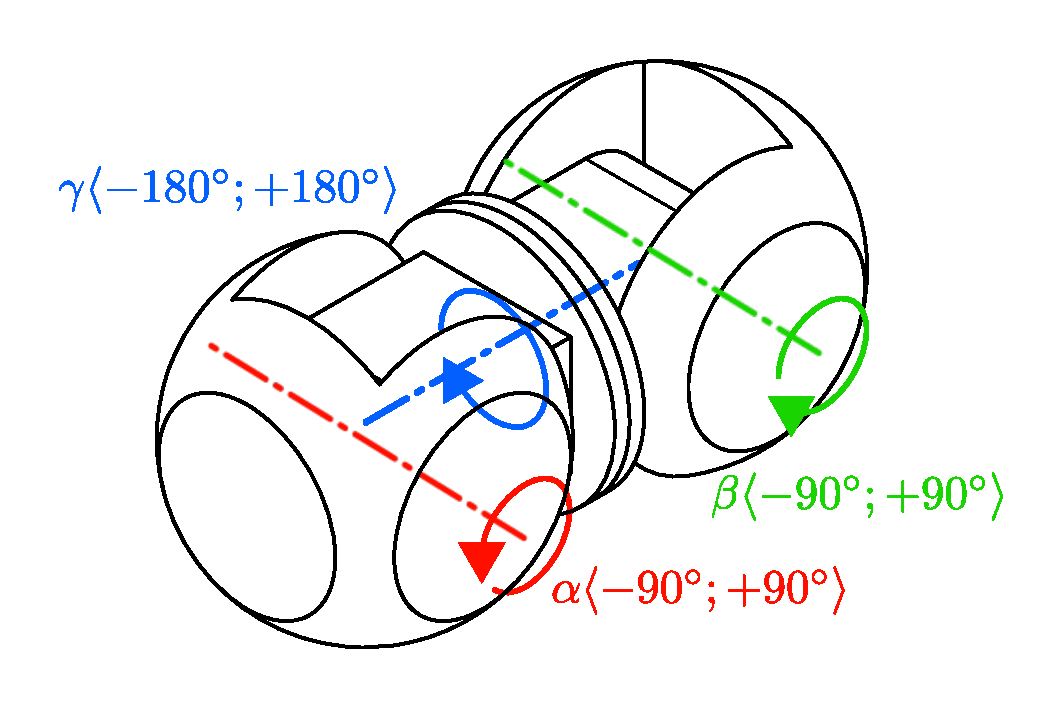
\includegraphics[width=0.6\textwidth]{pictures/module_angles.pdf}
    \caption[Stupne voľnosti modulu]{Schéma stupňov voľnosti modulu a smerov otáčania \cite{mrazekMasterThesis}.}
    \label{fig:module_angle}
\end{figure}

Ako bolo spomenuté vyššie, každý modul má schopnosť pripojiť sa k~iným modulom (a vytvoriť tak RoFIbota) alebo k~pasívnym prvkom pomocou \textit{konektorov} (\textit{dock}). Konektorový systém platformy RoFI je navrhnutý ako tzv. \textit{genderless}, čo umožňuje vzájomné spojenie ľubovoľných dvoch konektorov. 

\begin{figure}[hbt!]
    \centering
    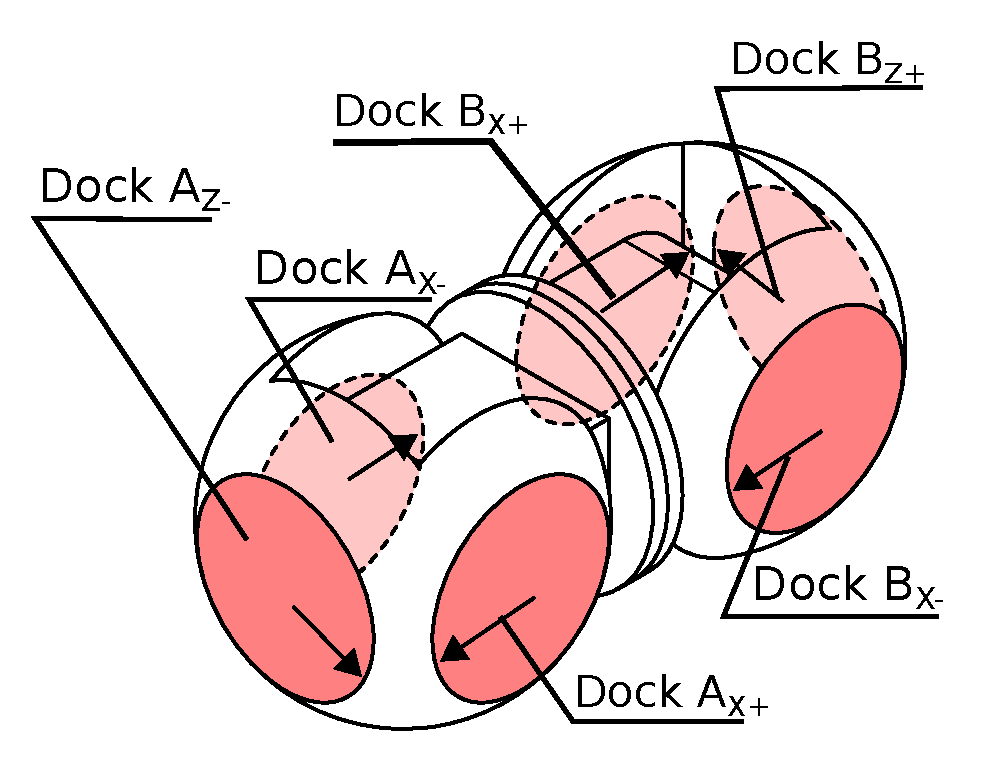
\includegraphics[width=0.6\textwidth]{pictures/dock_desc.pdf}
    \caption[Konektory modulu]{Schéma umiestnení konektorov na module a ich označenia. Šípky na konektoroch znázorňujú orientačné vektory \cite{mrazekMasterThesis}.}
    \label{fig:dock_desc}
\end{figure}

Každý modul obsahuje práve šesť konektorov, ktoré sú rozmiestnené po tri na každej topánke modulu. Konektor je okrem svojej polohy na module definovaný aj orientačným vektorom (viď obrázok \ref{fig:dock_desc}). 


Prepojenie je definované vzájomnou polohou orientačných vektorov konektorov spojenia. Konštrukcia konektorov dovoľuje ich prepojenie až v~štyroch rôznych polohách. 

Vzájomná poloha orientačných vektorov konektorov môže byť postupne $0\degree$, $90\degree$, $180\degree$ alebo $270\degree$ a tieto prepojenia sa označujú v~tomto poradí ako \textit{North}, \textit{East}, \textit{South} a \textit{West} (viď obrázok \ref{fig:dock_orientation}). 

\begin{figure}[hbt!]
    \centering
    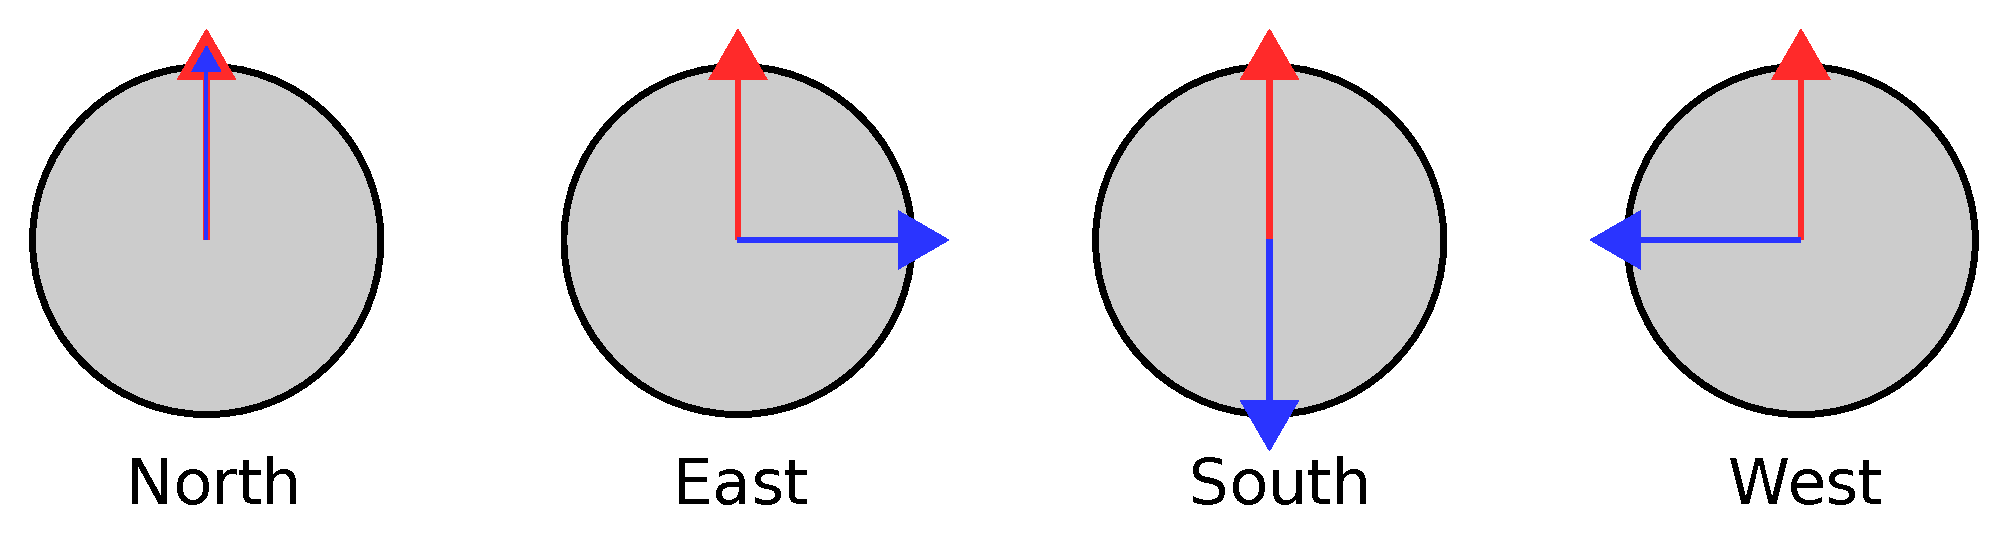
\includegraphics[width=0.6\textwidth]{pictures/dock_orientation.pdf}
    \caption[Možné spôsoby prepojenia konektorov modulu]{Schéma vzájomnej polohy orientačných vektorov spojených konektorov modulov. Červenou je označený konektor modulu, z~ktorého perspektívy spojenie označujeme. Modrá šípka je orientačný vektor druhého modulu. Poznámka: Nezáleží na výbere konektoru, z~ktorého perspektívy spojenie sledujeme \cite{mrazekMasterThesis}.}
    \label{fig:dock_orientation}
\end{figure}

\section{Popis RoFIbota}
\label{sec:rofibotSpec}
Vzájomné prepojenie modulov pomocou konektorov vytvára RoFIbotov. Parametre RoFIbota, ktoré ho definujú, sa dajú rozdeliť do dvoch kategórií:   
\begin{enumerate}
    \item tvar RoFIbota vzhľadom na jeho vnútornú štruktúru:
    \begin{itemize}[topsep=-5pt]
        \item množina modulov RoFIbota, 
        \item množina prepojení (hrán) modulov; 
    \end{itemize}
    
    \item poloha RoFIbota vzhľadom k~okolitému svetu: 
    \begin{itemize}[topsep=-5pt]
        \item natočenie celého RoFIbota vzhľadom na okolie, 
        \item umiestnenie RoFIbota do priestoru.  
    \end{itemize}
\end{enumerate}

\textit{Konfigurácia} RoFIbota je tvar RoFIbota vzhľadom na jeho vnútornú štruktúru, teda množina modulov a ich prepojení. Každý modul v~konfigurácii RoFIbota je definovaný jedinečným identifikátorom modulu a hodnotami všetkých troch stupňov voľnosti modulu. 

Jednotlivé hrany (prepojenia) v~konfigurácii RoFIbota sú definované identifikátormi spojených modulov, presným popisom konektorov, ktorými sú prepojené, a vzájomnou polohou spojených konektorov. 

\textit{Rekonfigurácia} RoFIbota je postupnosť validných krokov, ktorá u\-mož\-ní zmeniť počiatočnú konfiguráciu RoFIbota na cieľovú konfiguráciu RoFIbota. 
% ------------------------------------------------------ 1 ------------------------------------------------------






% ------------------------------------------------------ 2 ------------------------------------------------------
\chapter{Distribuovaná rekonfigurácia RoFIbotov}
\section{Formálne špecifikácie}
\label{sec:formalSpec}
Fyzický stav modulu a konfigurácie RoFIbota je nutné popísať z~formálneho hľadiska. Na základe tohto popisu je následne definovaná aj rekonfigurácia RoFIbota. 

\subsection{Modul}
\label{sec:formalSpecModul}
V~prvom rade je nutné definovať \textit{stav modulu}, ktorý je tvorený nasledujúcimi údajmi: 
\begin{itemize}
    \item \textit{id} -- unikátny identifikátor modulu, 
    \item $\alpha$ -- uhol otočenia topánky A~voči telu A~v~rozsahu $\interval[{-90\degree, 90\degree}]$,
    \item $\beta$ -- uhol otočenia topánky B voči telu B v~rozsahu $\interval[{-90\degree, 90\degree}]$,
    \item $\gamma$ -- uhol otočenia tela A~voči telu B v~rozsahu $\interval({-180\degree, 180\degree}]$,
    \item sedmica o~každom prepojení, ktoré daný modul má. 
\end{itemize} 

Ako už bolo popísané, spojenie definujú konektory, ktorými sú moduly spojené, a ich vzájomná poloha. Formálne ide o~nasledujúcu sedmicu: 
\begin{itemize}
    \item \textit{id1} -- unikátny identifikátor prvého modulu, 
    \item \textit{side1} -- strana prvého modulu, ktorou je spojený s~druhým modulom, 
    \item \textit{dock1} -- konektor prvého modulu, ktorý sa podieľa na prepojení,
    \item \textit{ori} -- orientácia spojených konektorov,
    \item \textit{dock2} -- konektor druhého modulu, ktorý sa podieľa na prepojení,
    \item \textit{side2} -- strana druhého modulu, ktorou je spojený s~prvým modulom, 
    \item \textit{id2} -- unikátny identifikátor druhého modulu. 
\end{itemize}
Zároveň platí, že tieto hodnoty sú z~nasledovných množín: $side1, side2 \in \{A, B\}$; $dock1, dock2 \in \{+X, -X, -Z\}$\footnote{Konektor $+Z$ budeme považovať za zhodný s~konektorom $-Z$. }; $ori \in \{N, E, S, W\}$.

\subsection{Konfigurácia}
\label{sec:formalSpecCfg}
Moduly sa spájajú do RoFIbotov a je nutné definovať si validitu konfigurácie. Konfigurácia RoFIbota je \textit{validná}, ak: 
\begin{itemize}
    \item každé prepojenie je vzájomné,
    \item každý konektor každého modulu sa podieľa na maximálne jednom prepojení, 
    \item všetky definované prepojenia je možné fyzicky vytvoriť (ich vzdialenosť dostatočne malá \cite{rofiCom}), 
    \item nesmie dochádzať k~žiadnej fyzickej kolízii modulov. 
\end{itemize}
Formálny popis výpočtu kolízií v~konfigurácii RoFIbota je podrobnejšie uvedený v~diplomovej práci \textit{Motion Planning for the RoFI Platform} \cite{vozarovaMasterThesis}. 

Keďže komunikácia medzi modulmi môže prebiehať po fyzickom spojení pomocou konektorov, ale aj bezdrôtovo, tak si zadefinujeme spojitosť RoFIbota. 

RoFIbot je \textit{spojitý}, ak medzi akýmikoľvek jeho dvomi modulmi existuje cesta tvorená modulmi a prepojeniami. To značí, že komunikácia medzi akýmikoľvek dvomi modulmi spojitého RoFIbota môže prebiehať výhradne fyzickými spojeniami (viď príklad spojitej a nespojitej konfigurácie na obrázku \ref{fig:exampleCfg}). 

\begin{figure}[hbt!]
    \centering
    \begin{subfigure}[b]{0.49\textwidth}
        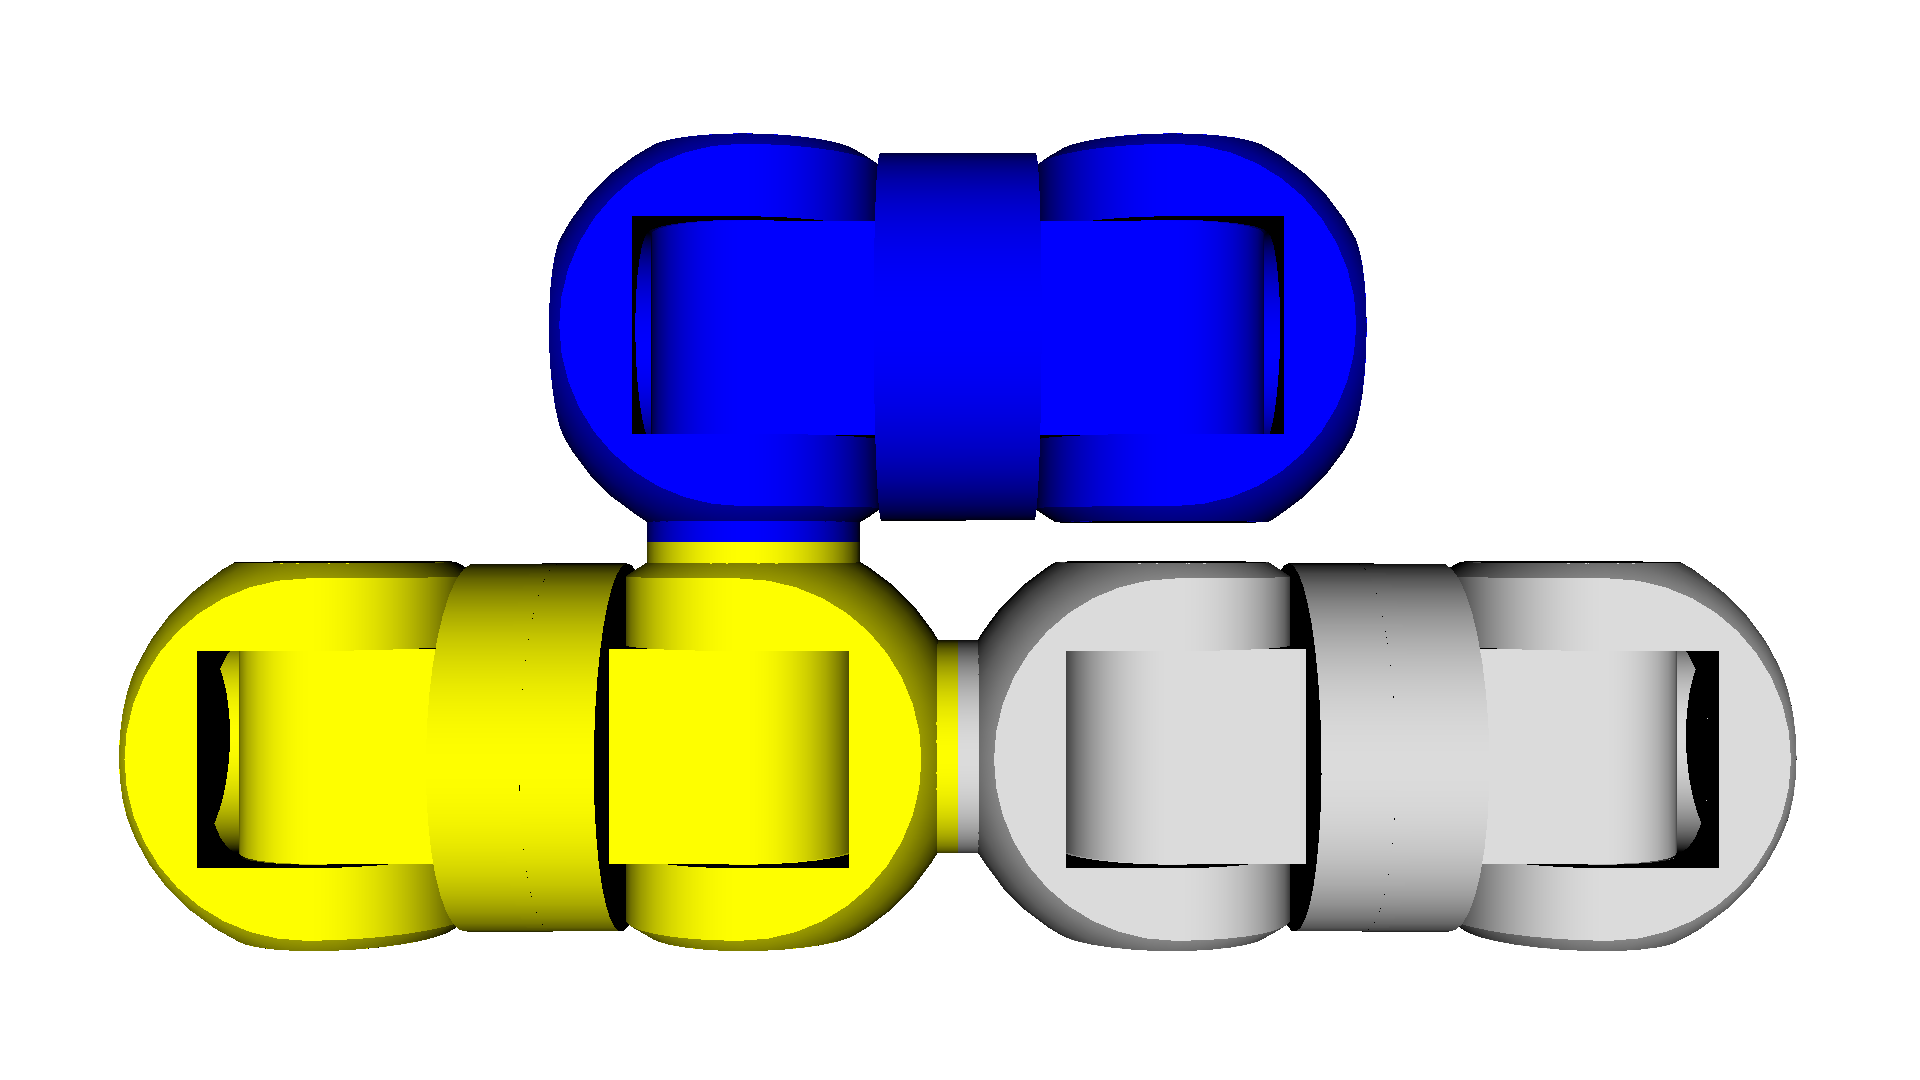
\includegraphics[width=\textwidth]{pictures/connected_rofibot.png}
        \caption[Spojitá konfigurácia.]{Spojitá konfigurácia}
        \label{fig:connectCfg}
    \end{subfigure}
    \begin{subfigure}[b]{0.49\textwidth}
        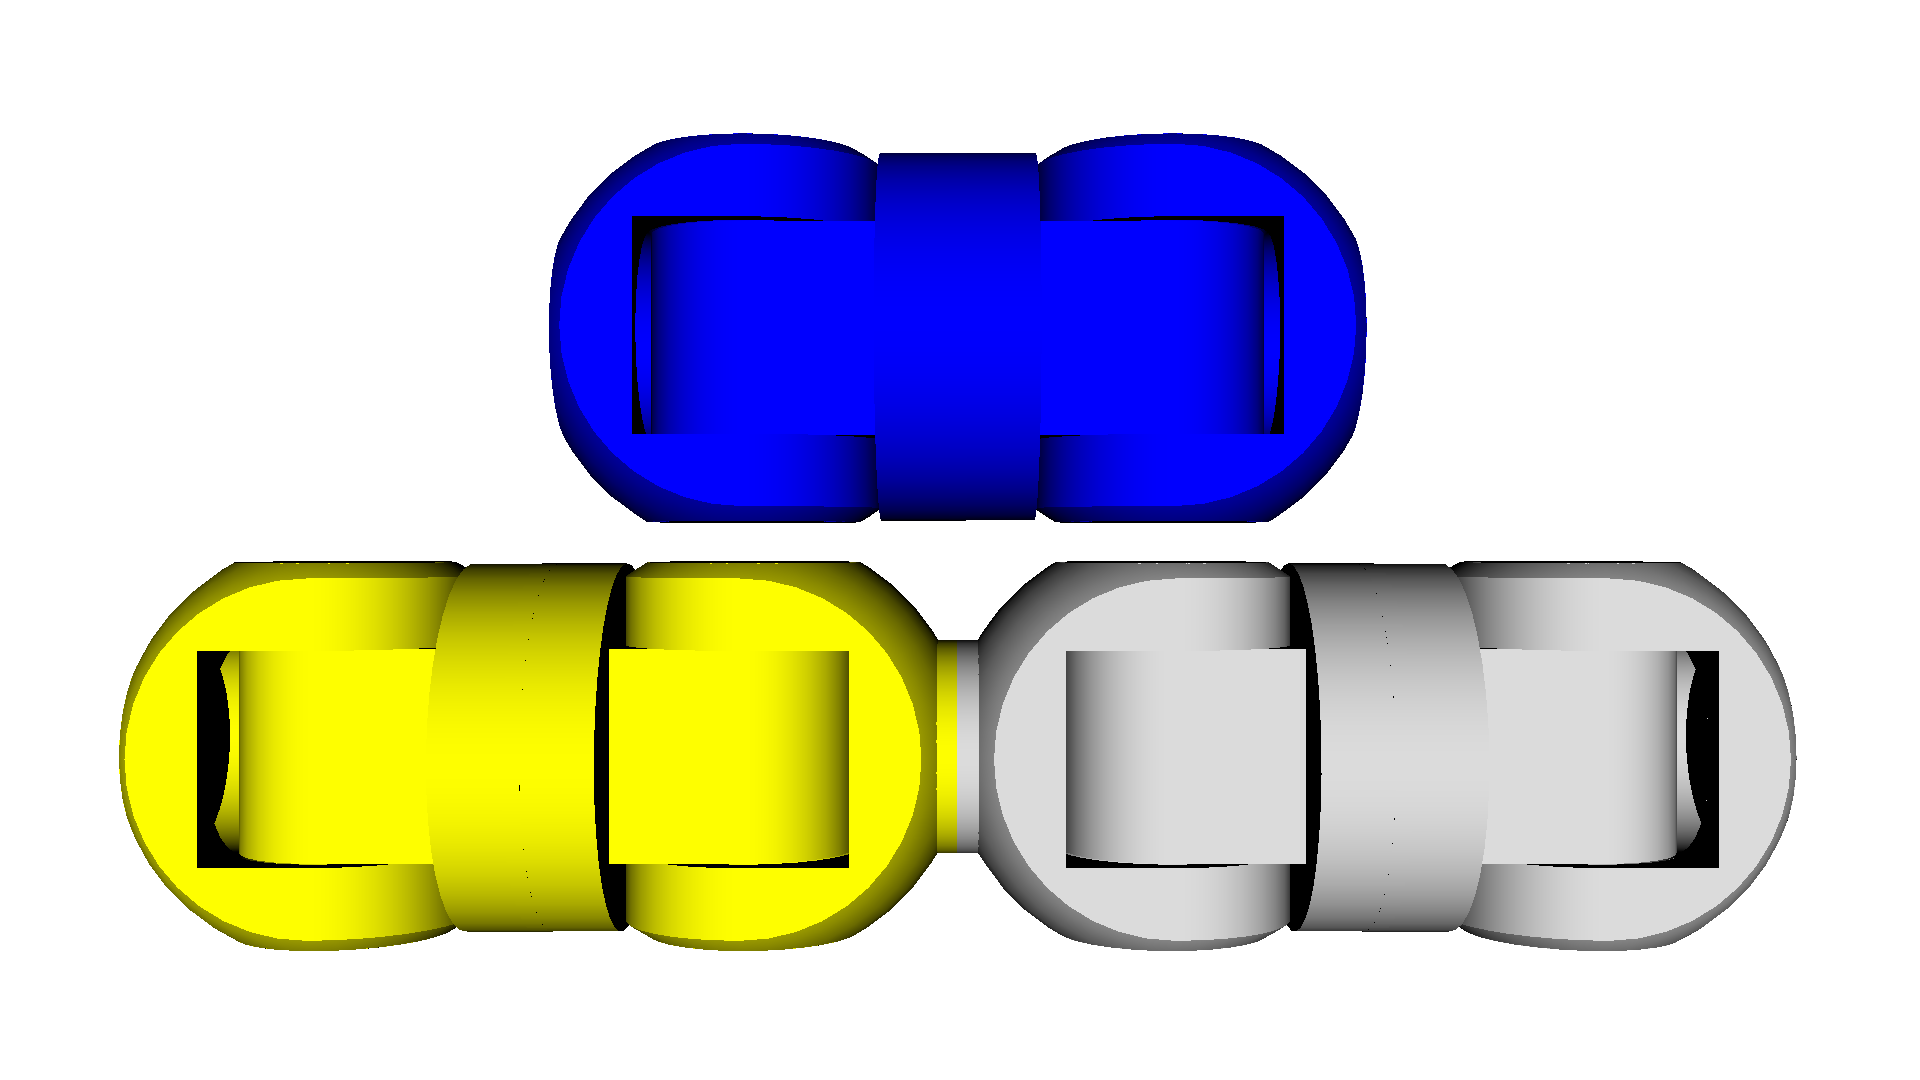
\includegraphics[width=\textwidth]{pictures/disconnected_rofibot.png}
        \caption[Nespojitá konfigurácia.]{Nespojitá konfigurácia}
        \label{fig:disconnectCfg}
    \end{subfigure}
    \caption[Príklad konfigurácie]{Príklad spojitej a nespojitej konfigurácie.}
    \label{fig:exampleCfg}
\end{figure}

Predpokladá sa, že každý modul je definovaný validne. To znamená, že údaje sú z~popísaných rozsahov a množín. Každá hrana je definovaná pre oba prepojené moduly, a to v~rovnakom tvare. Zároveň platí, že konfigurácia RoFIbota, ktorú popisujú dané stavy modulov, je spojitá a validná. 

\subsection{Rekonfigurácia RoFIbota}
\label{sec:formalRecfg}
Atomickou zmenou v~konfigurácii RoFIbota je \textit{akcia}, ktorá môže byť dvoch druhov. 

Prvým typom akcie je \textit{akcia rotácie}, ktorá sa deje na jednom z~modulov RoFIbota, a ide o~zmenu jedného z~parametrov $\alpha$, $\beta$ alebo $\gamma$. Je definovaná nasledovnými parametrami: 
\begin{itemize}
    \item \textit{id} -- \textit{id} modulu, ktorý mení jeden z~uhlov; $id \in \mathbb{Z}_0^+$, 
    \item \textit{joint} -- identifikácia stupňa voľnosti; $joint \in \{alfa, beta, gama\}$, 
    \item \textit{angle} -- orientovaný uhol, o~ktorý sa daný joint bude otáčať. 
\end{itemize}

Druhý typ akcie je \textit{akcia prepojenia}, ktorá definuje spojenie alebo rozpojenie dvoch modulov. Je definovaná nasledujúcimi parametrami: 
\begin{itemize}
    \item \textit{add} -- príznak, či ide o~spojenie alebo rozpojenie,
    \item \textit{edge} -- popis hrany, ktorá buď vznikne alebo zanikne (sedmica definovaná v~kapitole \ref{sec:moduleSpec}). 
\end{itemize}

Nie každú akciu je možné aplikovať na akúkoľvek konfiguráciu RoFIbota. \textit{Validná akcia} je akcia, ktorá spĺňa aj nasledujúce podmienky:
\begin{itemize}
    \item akcia rotácie: nesmie dôjsť ku kolízii s~inými modulmi (viď obrázok \ref{fig:rotationExample}), 
    \item akcia prepojenia: 
    \begin{itemize}[topsep=-5pt]
        \item oba konektory sa musia podieľať na spojení (príklad na obrázku \ref{fig:reconnectionExample}), 
        \item každý konektor sa podieľa na maximálne jednom spojení,
        \item konektory, ktoré sa majú prepojiť, musia byť fyzicky schopné prepojenia.
    \end{itemize}
\end{itemize}

\begin{figure}[hbt!]
    \centering
    \begin{subfigure}[b]{\textwidth}
        \centering
        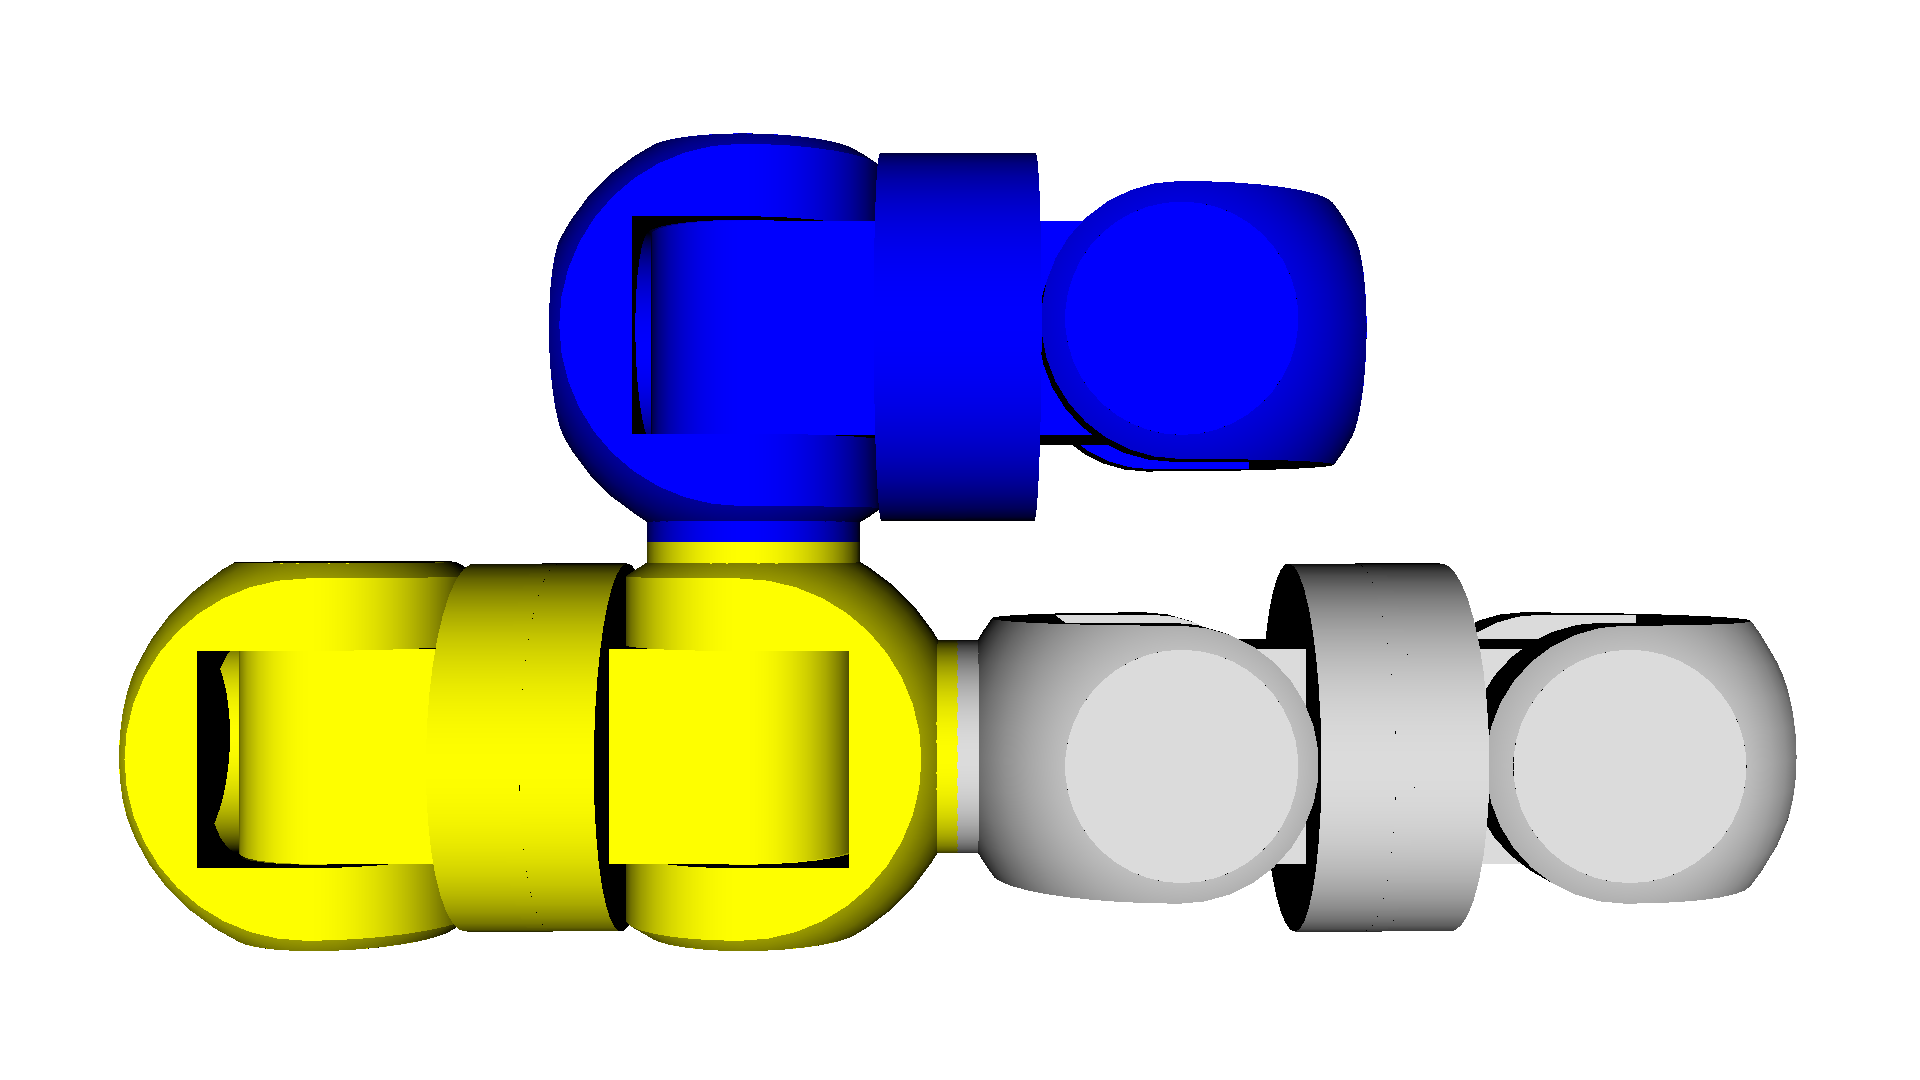
\includegraphics[width=0.47\textwidth]{pictures/rotation_example.png}
        \caption[Pred rotáciou]{Príklad konfigurácie pred rotáciou.}
    \end{subfigure}

    \begin{subfigure}[b]{0.47\textwidth}
        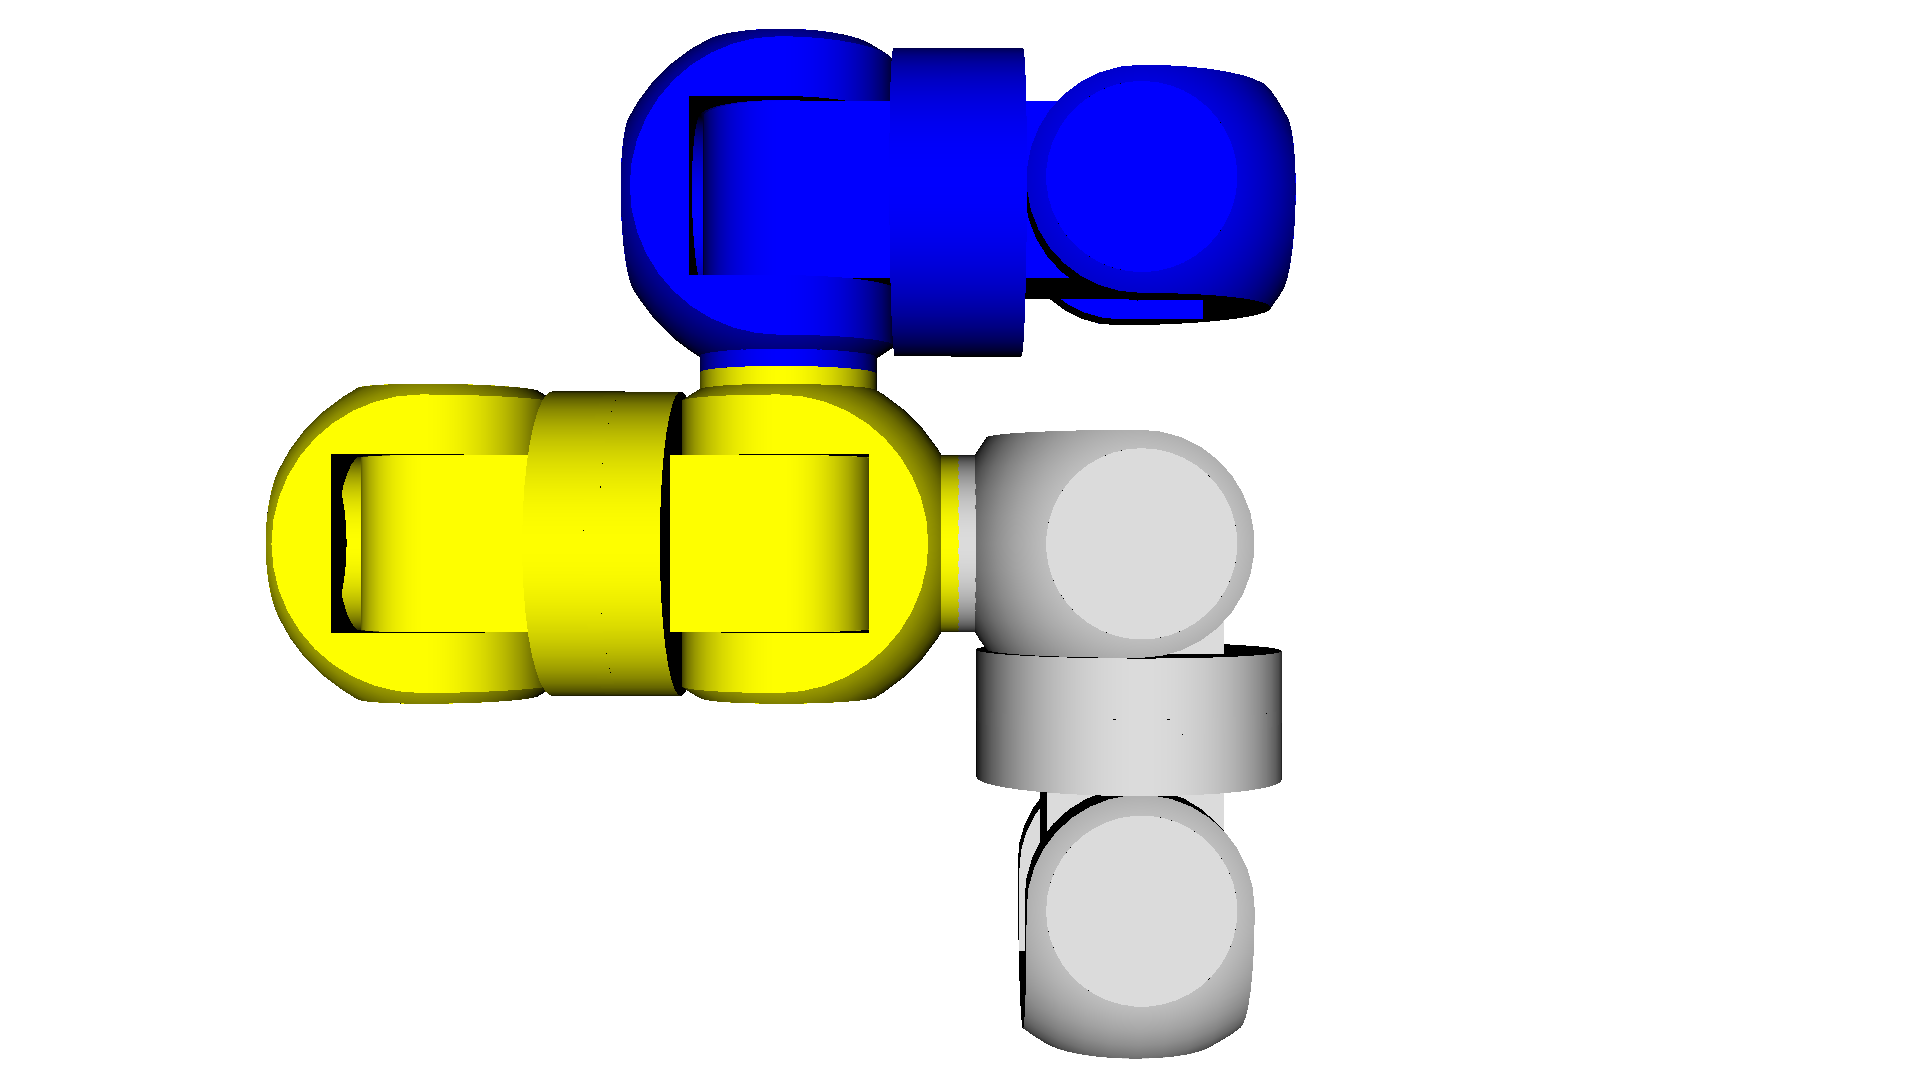
\includegraphics[width=\textwidth]{pictures/rotation_example_correct.png}
        \caption[Validná rotácia]{Validná rotácia modulu.}
    \end{subfigure}
    \begin{subfigure}[b]{0.47\textwidth}
        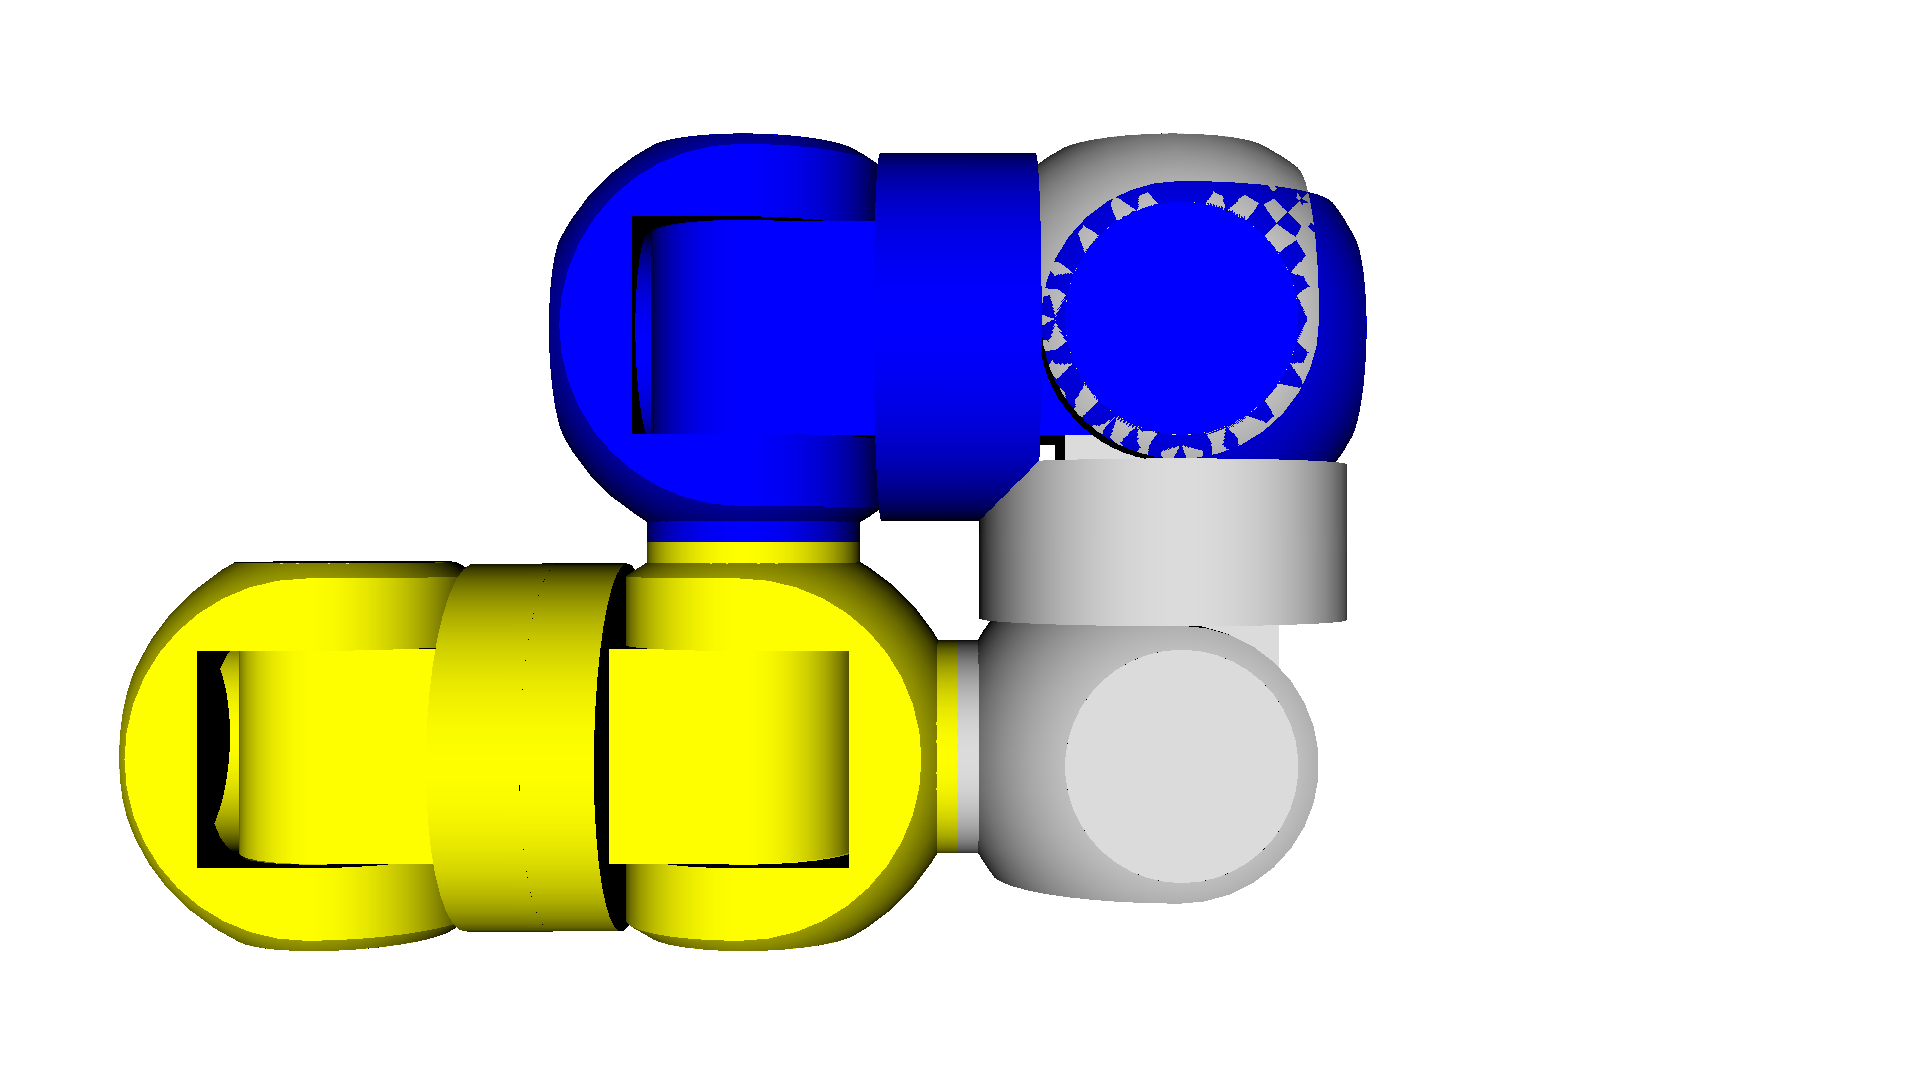
\includegraphics[width=\textwidth]{pictures/rotation_example_wrong.png}
        \caption[Nevalidná rotácia]{Nevalidná rotácia modulu.}
    \end{subfigure}
    \caption[Príklad akcie rotácie]{Príklad akcie rotácie (rotácia bieleho modulu o~$90\degree$ uhla $\gamma$).}
    \label{fig:rotationExample}
\end{figure}

\begin{figure}[hbt!]
    \centering
    \begin{subfigure}[b]{\textwidth}
        \centering
        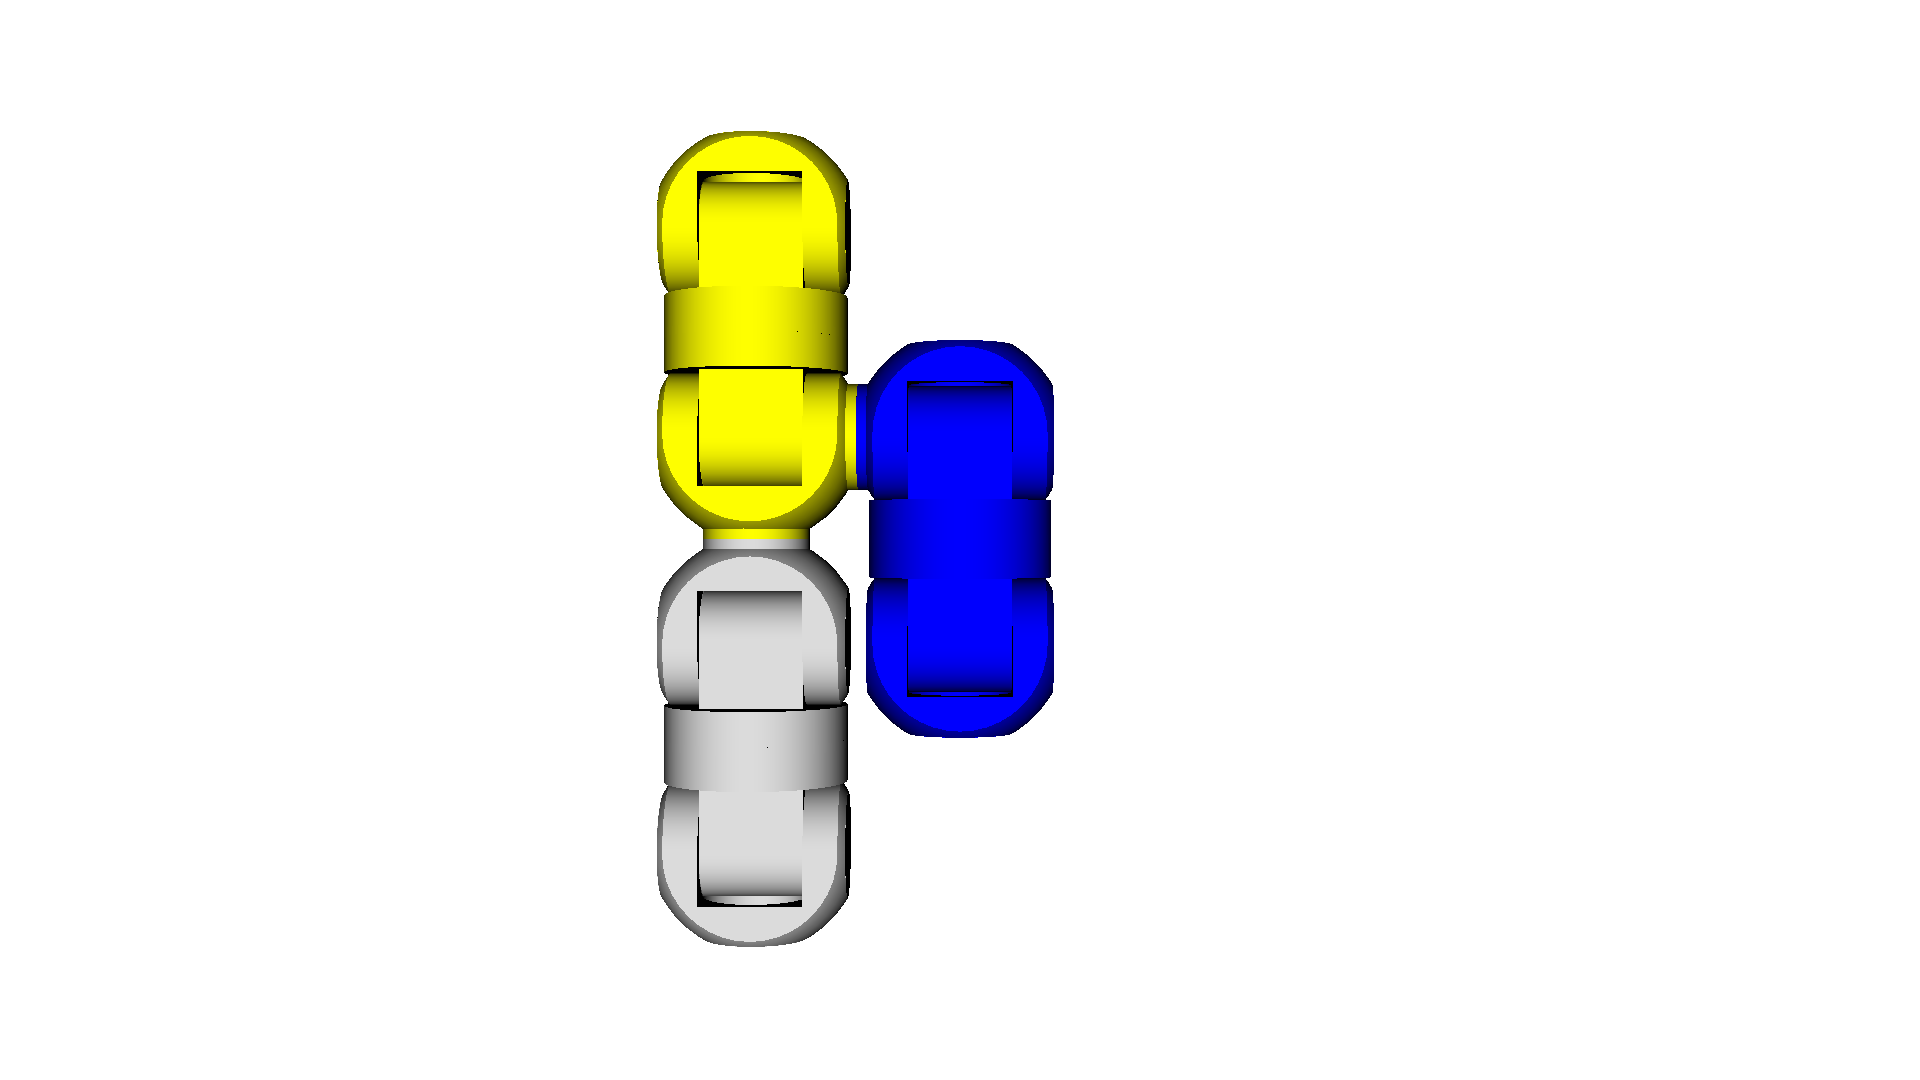
\includegraphics[width=0.8\textwidth]{pictures/reconnection_example.png}
        \caption[Pred prepojením]{Príklad konfigurácie pred vytvorením spojenia.}
    \end{subfigure}

    \begin{subfigure}[b]{0.47\textwidth}
        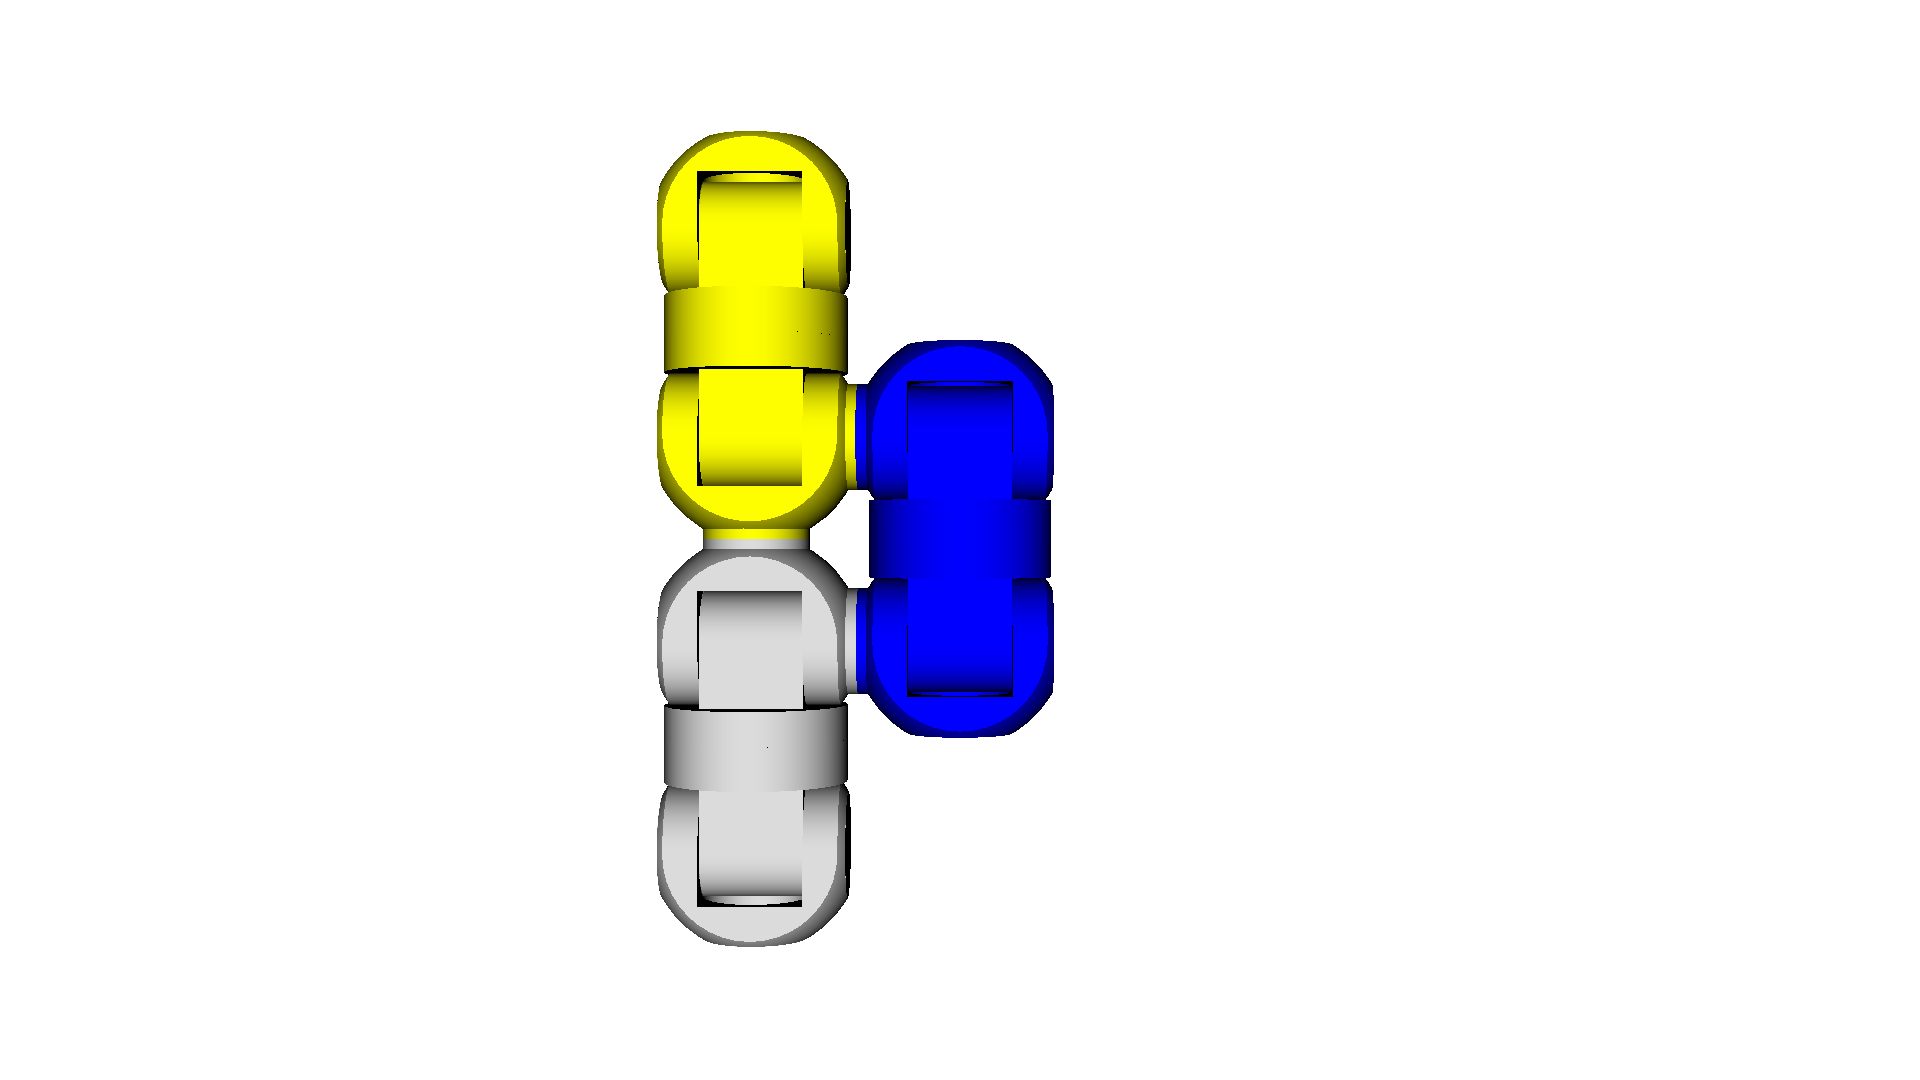
\includegraphics[width=\textwidth]{pictures/reconnection_example_correct.png}
        \caption[Validné spojenie]{Validné spojenie modulov \\(obidva sa podieľajú na spojení).}
    \end{subfigure}
    \begin{subfigure}[b]{0.47\textwidth}
        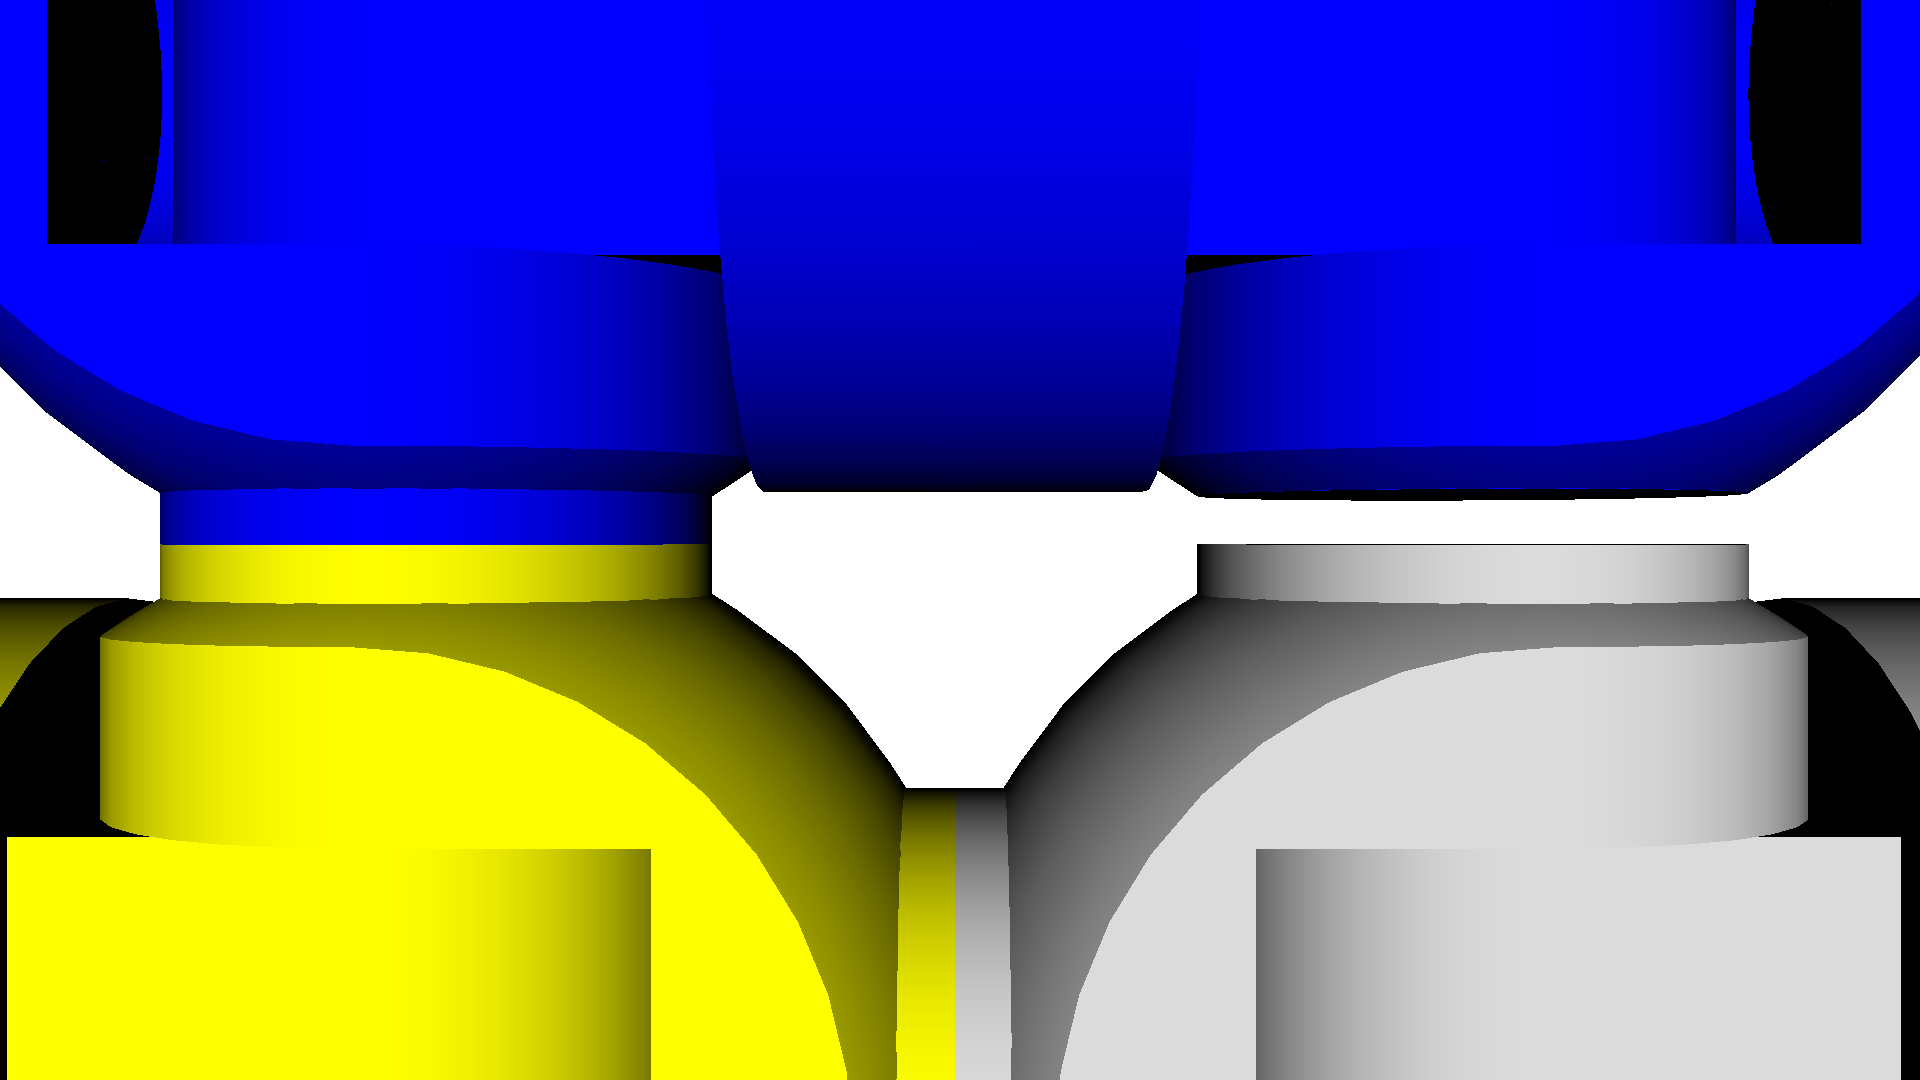
\includegraphics[width=\textwidth]{pictures/reconnection_example_wrong.png}
        \caption[Nevalidné prepojenie]{Nevalidné spojenie modulov \\(modrý sa nepodieľa na spojení).}
    \end{subfigure}
    \caption[Príklad akcie prepojenia]{Príklad akcie prepojenia (medzi bielym a modrým modulom).}
    \label{fig:reconnectionExample}
\end{figure}

% {0, 0, 136},
% {0, 0, 255},
% {119, 119, 255},
% {220, 220, 220},
% {255, 255, 136},
% {255, 255, 0},
% {119, 119, 0}};

\textit{Krok rekonfigurácie} je definovaný ako množina validných akcií. Poradie vykonávania akcií v~jednom krku rekonfigurácie nie je presne definované (prebiehajú zároveň, ale synchronizácia nikdy nie je úplne presná). 

Pre spojitých RoFIbotov musí platiť, že ak je konfigurácia pred krokom spojitá a validná, tak aj počas vykonávania kroku a po jeho vykonaní musí byť konfigurácia spojitá a validná. \textit{Validný krok} je krok rekonfigurácie taký, že konfigurácia je spojitá aj v~prípade, ak sa vykonajú iba všetky rozpojenia a žiadne iné akcie. 

Rekonfigurácia RoFIbota je definovaná ako postupnosť validných krokov. 

\section{Popis problému}
\label{sec:problemDesc}
Cieľom tejto práce je navrhnúť a implementovať algoritmy na rekonfiguráciu RoFIbotov, ktoré spĺňajú podmienky popísané v~tejto kapitole, a následne evaluovať výsledky. 

Diplomová práca \textit{Motion Planning for the RoFI Platform} \cite{vozarovaMasterThesis} popisuje rekonfiguráciu RoFIbotov z~centralizovaného pohľadu. To znamená, že algoritmy na rekonfiguráciu majú úplnú znalosť počiatočnej a cieľovej konfigurácie RoFIbota. 

Platforma RoFI je však navrhnutá ako distribuovaný systém, kde najmenšou stavebnou jednotkou je modul. Zároveň je platforma navrhnutá tak, že RoFIbot nemá žiadnu centralizovanú logickú jednotku, ktorá by dokázala riadiť rekonfiguráciu. 

Algoritmy navrhnuté v~tejto práci považujú modul za samostatnú entitu, ktorá na vstup dostane počiatočný a cieľový stav modulu, ktorý reprezentuje. Výstupom tejto entity je zoznam akcií, ktoré daný modul vykonal počas rekonfigurácie RoFIbota s~prihliadnutím na validitu a spojitosť. V~prípade, že sa RoFIbot nedokáže rekonfigurovať z~počiatočnej konfigurácie do cieľovej, tak implementované algoritmy túto skutočnosť dokážu identifikovať. 

Samotný modul nepozná celú konfiguráciu RoFIbota (dokonca pri veľkých konfiguráciách by znalosť celej konfigurácie mohla zaberať veľa miesta v~pamäti a nebola by potrebná). V~tejto práci má každý modul znalosť výhradne o~svojom stave, pričom každý ďalší údaj o~stave iných modulov vie získať výhradne posielaním si správ so susednými modulmi. 

Implementované algoritmy sú iba simuláciou reálnych rekonfigurácií RoFIbotov, teda nie je nutné striktne dodržiavať všetky fyzikálne zákonitosti reálneho sveta. V~praxi to znamená, že každý RoFIbot vykonáva svoju rekonfiguráciu „vo vákuu“, bez fyzických obmedzení (ako je napríklad podlaha či iné prekážky). Pri rekonfigurácii nehrajú rolu ani fyzikálne zákony (napríklad gravitácia). Zároveň musí platiť, že počas celej rekonfigurácie musí byť RoFIbot vo validnej a spojitej konfigurácii. 

To značí, že RoFIbot nemusí mať žiadne vnímanie okolitého sveta. Jedinými prekážkami v~pohyboch sú moduly samotné (ich poloha) a tú si entity vedia zistiť pomocou posielania si správ. 

Prínosom tejto práce je simulácia problému rekonfigurácie modulov v~distribuovanom prostredí. Súčasťou evaluácie navrhnutých a implementovaných algoritmov je aj porovnanie dĺžky výpočtov a počtu krokov rekonfigurácie distribuovaných algoritmov voči sebe aj voči vybraným algoritmom z~diplomovej práce \textit{Motion Planning for the RoFI Platform} \cite{vozarovaMasterThesis}. 

\section{Popis algoritmov na rekonfiguráciu}
\label{sec:algoDesc}
V~tejto práci sú navrhnuté a implementovaná dva algoritmy na rekonfiguráciu RoFIbotov, ktoré sa líšia hlavne prístupom k~znalosti celej konfigurácie RoFIbota. 

Prvý algoritmus využíva plnú znalosť celej konfigurácie RoFIbota. Zároveň využíva algoritmy na rekonfiguráciu navrhnuté a implementované v~diplomovej práci \textit{Motion Planning for the RoFI Platform} \cite{vozarovaMasterThesis}. Výsledok výpočtu rekonfigurácie pomocou motion planning je následne distribuovaný medzi moduly. 

Druhý algoritmus nevyžaduje znalosť celej konfigurácie, ale vďaka zasadeniu RoFIbota do súradnicovej sústavy je RoFIbot schopný rekonfigurácie pomocou komunikácie medzi modulmi. 

Pre oba algoritmy platí, že každý modul je reprezentovaný ako samostatná entita, ktorá má na začiatku znalosť o~svojom počiatočnom a cieľovom stave. Zároveň má možnosť komunikovať s~modulmi, s~ktorými je fyzicky prepojený. 

Môžeme predpokladať, že moduly dokážu komunikovať každý s~každým, nakoľko je RoFIbot v~každom momente rekonfigurácie spojitý. Problém posielania správ rieši nižšia softvérová vrstva, ktorá je už vo fyzických moduloch implementovaná a je možné ju využívať. 

\subsection{Algoritmus s~úplnou znalosťou konfigurácie}
\label{sec:motionPlanningAlgo}
V~počiatočnej fáze algoritmu rozošle každý z~modulov svoju počiatočnú a cieľovú konfiguráciu pomocou broadcastu. Tým zároveň každý modul získa stavy ostatných modulov RoFIbota. 

Aby mal modul úplnú konfiguráciu RoFIbota, je nutné získať hodnoty stupňov voľnosti $\alpha$, $\beta$ a $\gamma$ od všetkých modulov RoFIbota a zároveň je nutné mať plnú informáciu o~všetkých prepojeniach modulov. Všetky tieto údaje sú uložené v~stavoch modulov. Z~toho vyplýva, že po vzájomnom zdieľaní stavov medzi modulmi je každý modul schopný reprezentovať celú počiatočnú aj cieľovú konfiguráciu RoFIbota. To znamená, že každý modul je schopný vypočítať celú rekonfiguráciu, teda postupnosť validných krokov, pomocou algoritmov implementovaných v~diplomovej práci \textit{Motion Planning for the RoFI Platform} \cite{vozarovaMasterThesis}. 

Cieľom je, aby každý modul vypočítal rovnakú postupnosť krokov. To znamená, že z~algoritmov implementovaných v~spomínanej diplomovej práci je nutné vybrať deterministický algoritmus, ktorým je buď \textit{BFS} alebo \textit{A*} (algoritmus \textit{RRT} nie je deterministický). Výsledky porovnania týchto dvoch algoritmov v~spomínanej diplomovej práci ukazujú, že algoritmus \textit{A*} je časovo rýchlejší ako algoritmus \textit{BFS}. Z~tohto dôvodu budú moduly využívať algoritmus \textit{A*}. 

Pre algoritmus \textit{A*} je nutné vybrať ako jeho parameter heuristiku (pre každý modul rovnakú). Zároveň budú moduly počítať postupnosť krokov tak, aby sa v~každom kroku udiala výhradne jedna validná akcia, čo je možné vďaka implementácii limitu na maximálny počet akcií, ktoré je možné vykonať v~jednom kroku rekonfigurácie. Obmedzenie na jednu akciu v~kroku je vhodné hlavne kvôli optimalizácii krokov rekonfigurácie, ktorá je popísaná neskôr. 

Po výpočte má každý modul vypočítanú tú istú postupnosť krokov, ktoré sa majú vykonávať na to, aby sa RoFIbot mohol rekonfigurovať, alebo dokáže identifikovať, že rekonfigurácia nie je možná. 

Ak nie je rekonfigurácia možná, tak tento fakt identifikuje už výpočet algoritmu \textit{A*}. Preto aj výpočet algoritmu navrhnutého pre túto prácu dokáže túto skutočnosť identifikovať a vo výpočte už ďalej nepokračuje. 

Ak je rekonfigurácia validná, tak následne budú moduly túto postupnosť optimalizovať. Optimalizácia je vhodná hlavne z~dôvodu zrýchlenia fyzickej rekonfigurácie RoFIbota, čiže chceme, aby sa viacero krokov pôvodnej postupnosti vykonávalo súčasne. 

Optimalizácia bude opäť iba heuristikou a nezaručuje nájdenie optimálneho riešenia (vzhľadom na počet krokov rekonfigurácie) paralelizácie krokov, ale zaručuje, že nájdené riešenie ostane validnou rekonfiguráciou RoFIbota. Táto optimalizácia spočíva v~dvoch fázach, a to v~spájaní krokov a v~ich výmenách. Tieto optimalizácie je možné robiť výhradne na dvoch krokoch, ktoré po sebe nasledujú. 

Navrhnutá optimalizácia intuitívne prebieha tak, že pospája čo najviac krokov dohromady a následne sa novovzniknuté kroky pokúsi povymieňať, aby bola postupnosť krokov rekonfigurácie naďalej validná. Toto sa opakuje, až kým sa vo fáze spájania nevykoná žiadna zmena. 

Z~formálneho hľadiska si pre lepšiu orientáciu zadefinujme $\mathcal{C}_i$ ako konfiguráciu RoFIbota po $i$-tom kroku. Teda $\mathcal{C}_0$ je počiatočná konfigurácia. Ďalej si definujme $\mathcal{S}_i$ ako $i$-ty krok rekonfigurácie. Zároveň, nech je operátor \lstinline{<*>} definovaný ako aplikácia kroku $\mathcal{S}$ na konfiguráciu $\mathcal{C}$, teda platí $\mathcal{S}_{i + 1}$ \lstinline{<*>} $\mathcal{C}_i = \mathcal{C}_{i + 1}$. Nech $\mathcal{S}'_i = \mathcal{S}_i \cup \mathcal{S}_{i + 1}$. 

\textit{Spojenie krokov} $\mathcal{S}_i$ a $\mathcal{S}_{i + 1}$ je možné iba ak platí, že $\mathcal{S}'_i$ je validný krok. Zároveň musí platiť, že ak zjednotenie krokov $\mathcal{S}_i$ a $\mathcal{S}_{i + 1}$ aplikujeme na konfiguráciu $\mathcal{C}_{i - 1}$, tak výsledok bude rovnaký, ako keby sme ich aplikovali postupne. To je ekvivalentne zapísané nasledovne: 
\begin{align}
\label{align:stepJoin}
\mathcal{S}_{i + 1} \lstinline{<*>} (\mathcal{S}_i \lstinline{<*>} \mathcal{C}_{i - 1}) = \mathcal{S}'_i \lstinline{<*>} \mathcal{C}_{i - 1}. 
\end{align}

Rovnosť \ref{align:stepJoin} však popisuje iba spojenie dvoch krokov. Navrhnutý algoritmus sa snaží minimalizovať počet krokov celkovo, a teda je potrebné systematicky spájať viaceré kroky. 

Toto spájanie prebieha nasledovne: Postupne sa prechádza každý index krokov od $1$ až po predposledný krok rekonfigurácie. Ak sa kroky $\mathcal{S}_i$ a $\mathcal{S}_{i + 1}$ dajú spojiť, tak sa postupnosť upraví tak, že tieto dva kroky sa vymažú, na ich miesto sa vloží $\mathcal{S}'_i$ (ostatné kroky sa následne prečíslujú) a pokračuje sa opäť testovaním spájania krokov na indexoch $i$ (novovytvorený krok $\mathcal{S}'_i$) a $i + 1$. Tento postup je popísaný aj v~algoritme~\ref{algorithm:stepJoin}. 

\begin{algorithm}
    \caption{joinSteps}
    \label{algorithm:stepJoin}
    \DontPrintSemicolon
    \SetKwInOut{Input}{vstup}\SetKwInOut{Output}{výstup}
    \SetKwData{CurrIndex}{i}
    \SetKwData{NextIndex}{\CurrIndex + 1}
    \SetKwData{JoinStep}{$\mathcal{S}'$}
    \SetKwData{Cfg}{$\mathcal{C}_{\CurrIndex - 1}$}
    \SetKwData{Steps}{stepVector}
    \Input{\ \Steps\ -- postupnosť krokov rekonfigurácie.}
    \Output{\ \Steps\ -- postupnosť krokov rekonfigurácie taká, že žiadne dva susedné kroky sa už nedajú spojiť.}
    
    \CurrIndex $\leftarrow$ 1\;
    \While{\CurrIndex < $|\Steps|$}{
        \JoinStep $\leftarrow \mathcal{S}_\CurrIndex$ $\cup$ $\mathcal{S}_\NextIndex$\;
        
        \eIf{\upshape $\mathcal{S}_\NextIndex$ \lstinline{<*>} ($\mathcal{S}_\CurrIndex$ \lstinline{<*>} \Cfg) $=$ \JoinStep \lstinline{<*>} \Cfg\ {\bf and} \JoinStep \textit{je validný}}{
            vymaž $\mathcal{S}_\NextIndex$ a $\mathcal{S}_\CurrIndex$\;
            na index \CurrIndex vlož krok \JoinStep\;
        }{
            \CurrIndex $\leftarrow$ \NextIndex\;
        }
    }
\end{algorithm}

\textit{Výmena krokov} $\mathcal{S}_i$ a $\mathcal{S}_{i + 1}$ je definovaná tak, že sa vymení poradie týchto dvoch krokov. Táto výmena musí spĺňať nasledujúce podmienky: Ak sa najskôr vykoná krok $\mathcal{S}_{i + 1}$, a až potom krok $\mathcal{S}_i$, tak bude výsledok rovnaký ako pri vykonaní krokov v~pôvodnom poradí. Zároveň však musí platiť, že aj vymenené poradie krokov je validné a dodržiavajú sa podmienky na validný krok (napr. spojitosť RoFIbota). Formálne je prvá podmienka definovaná nasledovne: 
\begin{align}
\label{align:stepSwap}
\mathcal{S}_{i + 1} \lstinline{<*>} (\mathcal{S}_i \lstinline{<*>} \mathcal{C}_{i - 1}) = \mathcal{S}_i \lstinline{<*>} (\mathcal{S}_{i + 1} \lstinline{<*>} \mathcal{C}_{i - 1}). 
\end{align}

Rovnosť \ref{align:stepSwap} popisuje iba výmenu dvoch krokov. Cieľom algoritmu však bude v~časti výmeny krokov vymeniť ich viacero, nakoľko tieto výmeny môžu umožniť ďalšie spájania krokov. 

Výmeny prebiehajú nasledovne: Postupne sa prechádza každý index krokov od $1$ až po predposledný krok rekonfigurácie. Ak sa kroky $\mathcal{S}_i$ a $\mathcal{S}_{i + 1}$ dajú vymeniť, tak sa vymenia. Následne sa pokračuje testovaním výmeny pre krok na indexe $i + 1$ a $i + 2$. Tento postup je uvedený pomocou pseudokódu v~algoritme~\ref{algorithm:stepSwap}. 

\begin{algorithm}
    \caption{swapSteps}
    \label{algorithm:stepSwap}
    
    \DontPrintSemicolon
    \SetKwInOut{Input}{vstup}\SetKwInOut{Output}{výstup}
    \SetKwData{CurrIndex}{i}
    \SetKwData{NextIndex}{\CurrIndex + 1}
    \SetKwData{Steps}{stepVector}
    \SetKwData{Cfg}{$\mathcal{C}_{\CurrIndex - 1}$}
    \Input{\ \Steps\ -- postupnosť krokov rekonfigurácie.}
    \Output{\ \Steps\ -- postupnosť krokov rekonfigurácie po výmene krokov.}
    
    \For{\CurrIndex $\leftarrow 1$ \KwTo $|\Steps|$}{
        \If{\upshape $\mathcal{S}_\CurrIndex$ \lstinline{<*>} ($\mathcal{S}_\NextIndex$ \lstinline{<*>} \Cfg) $=$ $\mathcal{S}_\NextIndex$ \lstinline{<*>} ($\mathcal{S}_\CurrIndex$ \lstinline{<*>} \Cfg) \\ \hspace{12}{\bf and} $\mathcal{S}_\NextIndex$ a $\mathcal{S}_\CurrIndex$ \textit{validné v~tomto poradí}}{
            vymeň $\mathcal{S}_\CurrIndex$ a $\mathcal{S}_\NextIndex$\;
        }
    }
\end{algorithm}

Celá optimalizácia prebieha nasledovným spôsobom: V~prvom rade sa vykoná spájanie krokov. Následne sa opakuje výmena krokov a spájanie krokov, a to dovtedy, kým spájanie krokov vykoná nejakú zmenu. Táto optimalizácia je znázornená aj v~algoritme~\ref{algorithm:algo1}. 

\begin{algorithm}
    \caption{Optimalizácia krokov rekonfigurácie. }
    \label{algorithm:algo1}
    
    \DontPrintSemicolon
    \SetKwInOut{Input}{vstup}\SetKwInOut{Output}{výstup}
    \SetKwData{Steps}{stepVector}
    \SetKwRepeat{Do}{do}{while}
    \Input{\ \Steps\ -- postupnosť krokov na optimalizáciu.}
    \Output{\ \Steps\ -- optimalizovaná postupnosť krokov.}
    
    \Steps $\leftarrow$ joinSteps(\Steps)\;
    \Do{\Steps sa zmenil po spojení krokov}{
        \Steps $\leftarrow$ swapSteps(\Steps)\;
        \Steps $\leftarrow$ joinSteps(\Steps)\;
    }
\end{algorithm}

Vyššie popísaná optimalizácia vždy skončí v~konečnom čase. Algoritmus \ref{algorithm:stepJoin} po každom cykle buď zvýši hodnotu aktuálneho indexu, alebo zníži celkový počet krokov, teda v~každom prípade sa zníži hodnota rozdielu medzi celkovým počtom krokov a aktuálnym indexom. To znamená, že v~konečnom čase sa dostane na hodnotu menšiu ako $1$, teda cyklus skončí. V~algoritme \ref{algorithm:stepSwap} je využitý cyklus $for$, ktorý zaručene skončí v~konečnom čase. 

Ostáva dokázať, že algoritmus \ref{algorithm:algo1} skončí. Cyklus je podmienený výhradne tým, či nastane zmena po spájaní krokov. Po každom prechode cyklu (okrem posledného) vieme, že sa počet krokov určite zmenšil (nastalo aspoň jedno spojenie), takže v~konečnom čase sa buď spojenie neuskutoční alebo bude počet krokov rovný $1$, čo bude znamenať, že v~nasledujúcom kroku sa nebude môcť vykonať spojenie krokov, čím sa ukončí cyklus. 

Táto optimalizácia je korektná, nakoľko sa vykonávajú iba korektné akcie spojenia a výmeny, ktoré sa vždy kontrolujú pred ich vykonaním. Preto ak optimalizácia dostane na vstup korektnú postupnosť krokov, tak na výstup vráti optimalizovanú korektnú postupnosť krokov. 

Vyššie popísaný algoritmus prebieha na každom z~modulov, teda každý z~nich optimalizoval vypočítanú postupnosť krokov rekonfigurácie. Nakoľko je každý algoritmus deterministický, tak každý z~nich vypočíta rovnaký výsledok. Preto sa môže začať fyzická rekonfigurácia, ktorá je daná postupnosťou krokov, teda každý modul vie, v~ktorom čase má vykonať akú zmenu. 

Moduly vzájomne komunikujú a posielajú si informácie, že už vykonali daný krok a môže nastať ďalší. Prvý krok môže nastať hneď ako každý dopočíta optimalizáciu. Ak modul vykoná fyzickú akciu v~$i$-tom kroku, tak pošle správu každému modulu v~$(i + 1)$-tom kroku, že daný modul už vykonal $i$-ty krok. Modul začne vykonávať fyzickú akciu v~$(i + 1)$-tom kroku až v~prípade, ak dostal správu od každého modulu, ktorý mal vykonávať akciu v~$i$-tom kroku. Ak má modul vykonávať viacero akcií v~jednom kroku, tak správy posiela až po vykonaní všetkých akcií. Po vykonaní akcií v~poslednom kroku rekonfigurácie sa správy už neposielajú. 

Tento algoritmus je navrhnutý tak, že ak niektorý z~modulov z~nejakého dôvodu nie je schopný výpočtov, tak je možné výsledky mu iba poslať. Zároveň je navrhnutý tak, aby sa dal ľahko adaptovať na zmeny a vylepšenia, pričom niektoré sú popísané v~kapitole \ref{sec:future}.  

\subsection{Algoritmus s~čiastočnou znalosťou konfigurácie}
\label{sec:distributedAlgo}
Druhý implementovaný algoritmus nepotrebuje znalosť celej konfigurácie RoFIbota. Z~intuitívneho pohľadu algoritmus spočíva v~tom, že sa v~každom kroku vyberie modul, ktorý sa pokúsi priblížiť svoj stav bližšie k~cieľovému stavu. Pod pojmom priblížiť sa rozumie buď otočenie niektorým zo stupňov voľnosti, odpojenie niektorej z~aktuálnych hrán, ktoré v~koncovom stave nie sú, alebo pripojenie k~inému modulu tak, aby tvorili hranu, ktorá je v~koncovom stave modulu. Nakoľko je RoFIbot vsadený do 3D mriežky, tak v~tomto algoritme používame súradnicový systém s~predpokladom, že veľkosť hrany mriežky je $1$\,cm. 

Spôsob zavedenia súradnicového systému a aj algoritmus na výpočet súradníc pre ostatné moduly sú prevzaté z~diplomovej práce \textit{Motion Planning for the RoFI Platform} \cite{vozarovaMasterThesis}. Základom je definovanie osí súradnicového systému, ktoré sú určené podľa strany A~modulu s~najnižším \textit{id}, tak ako je to zobrazené na obrázku \ref{fig:moduleAxis}. 

\begin{figure}[hbt!]
    \centering
    \begin{subfigure}[b]{0.47\textwidth}
        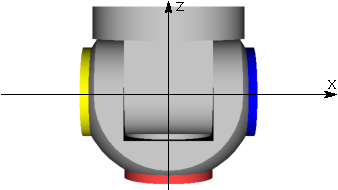
\includegraphics[width=\textwidth]{pictures/module_dock_identification.pdf}
        \caption[Pohľad spredu]{Pohľad spredu.}
    \end{subfigure}
    \begin{subfigure}[b]{0.47\textwidth}
        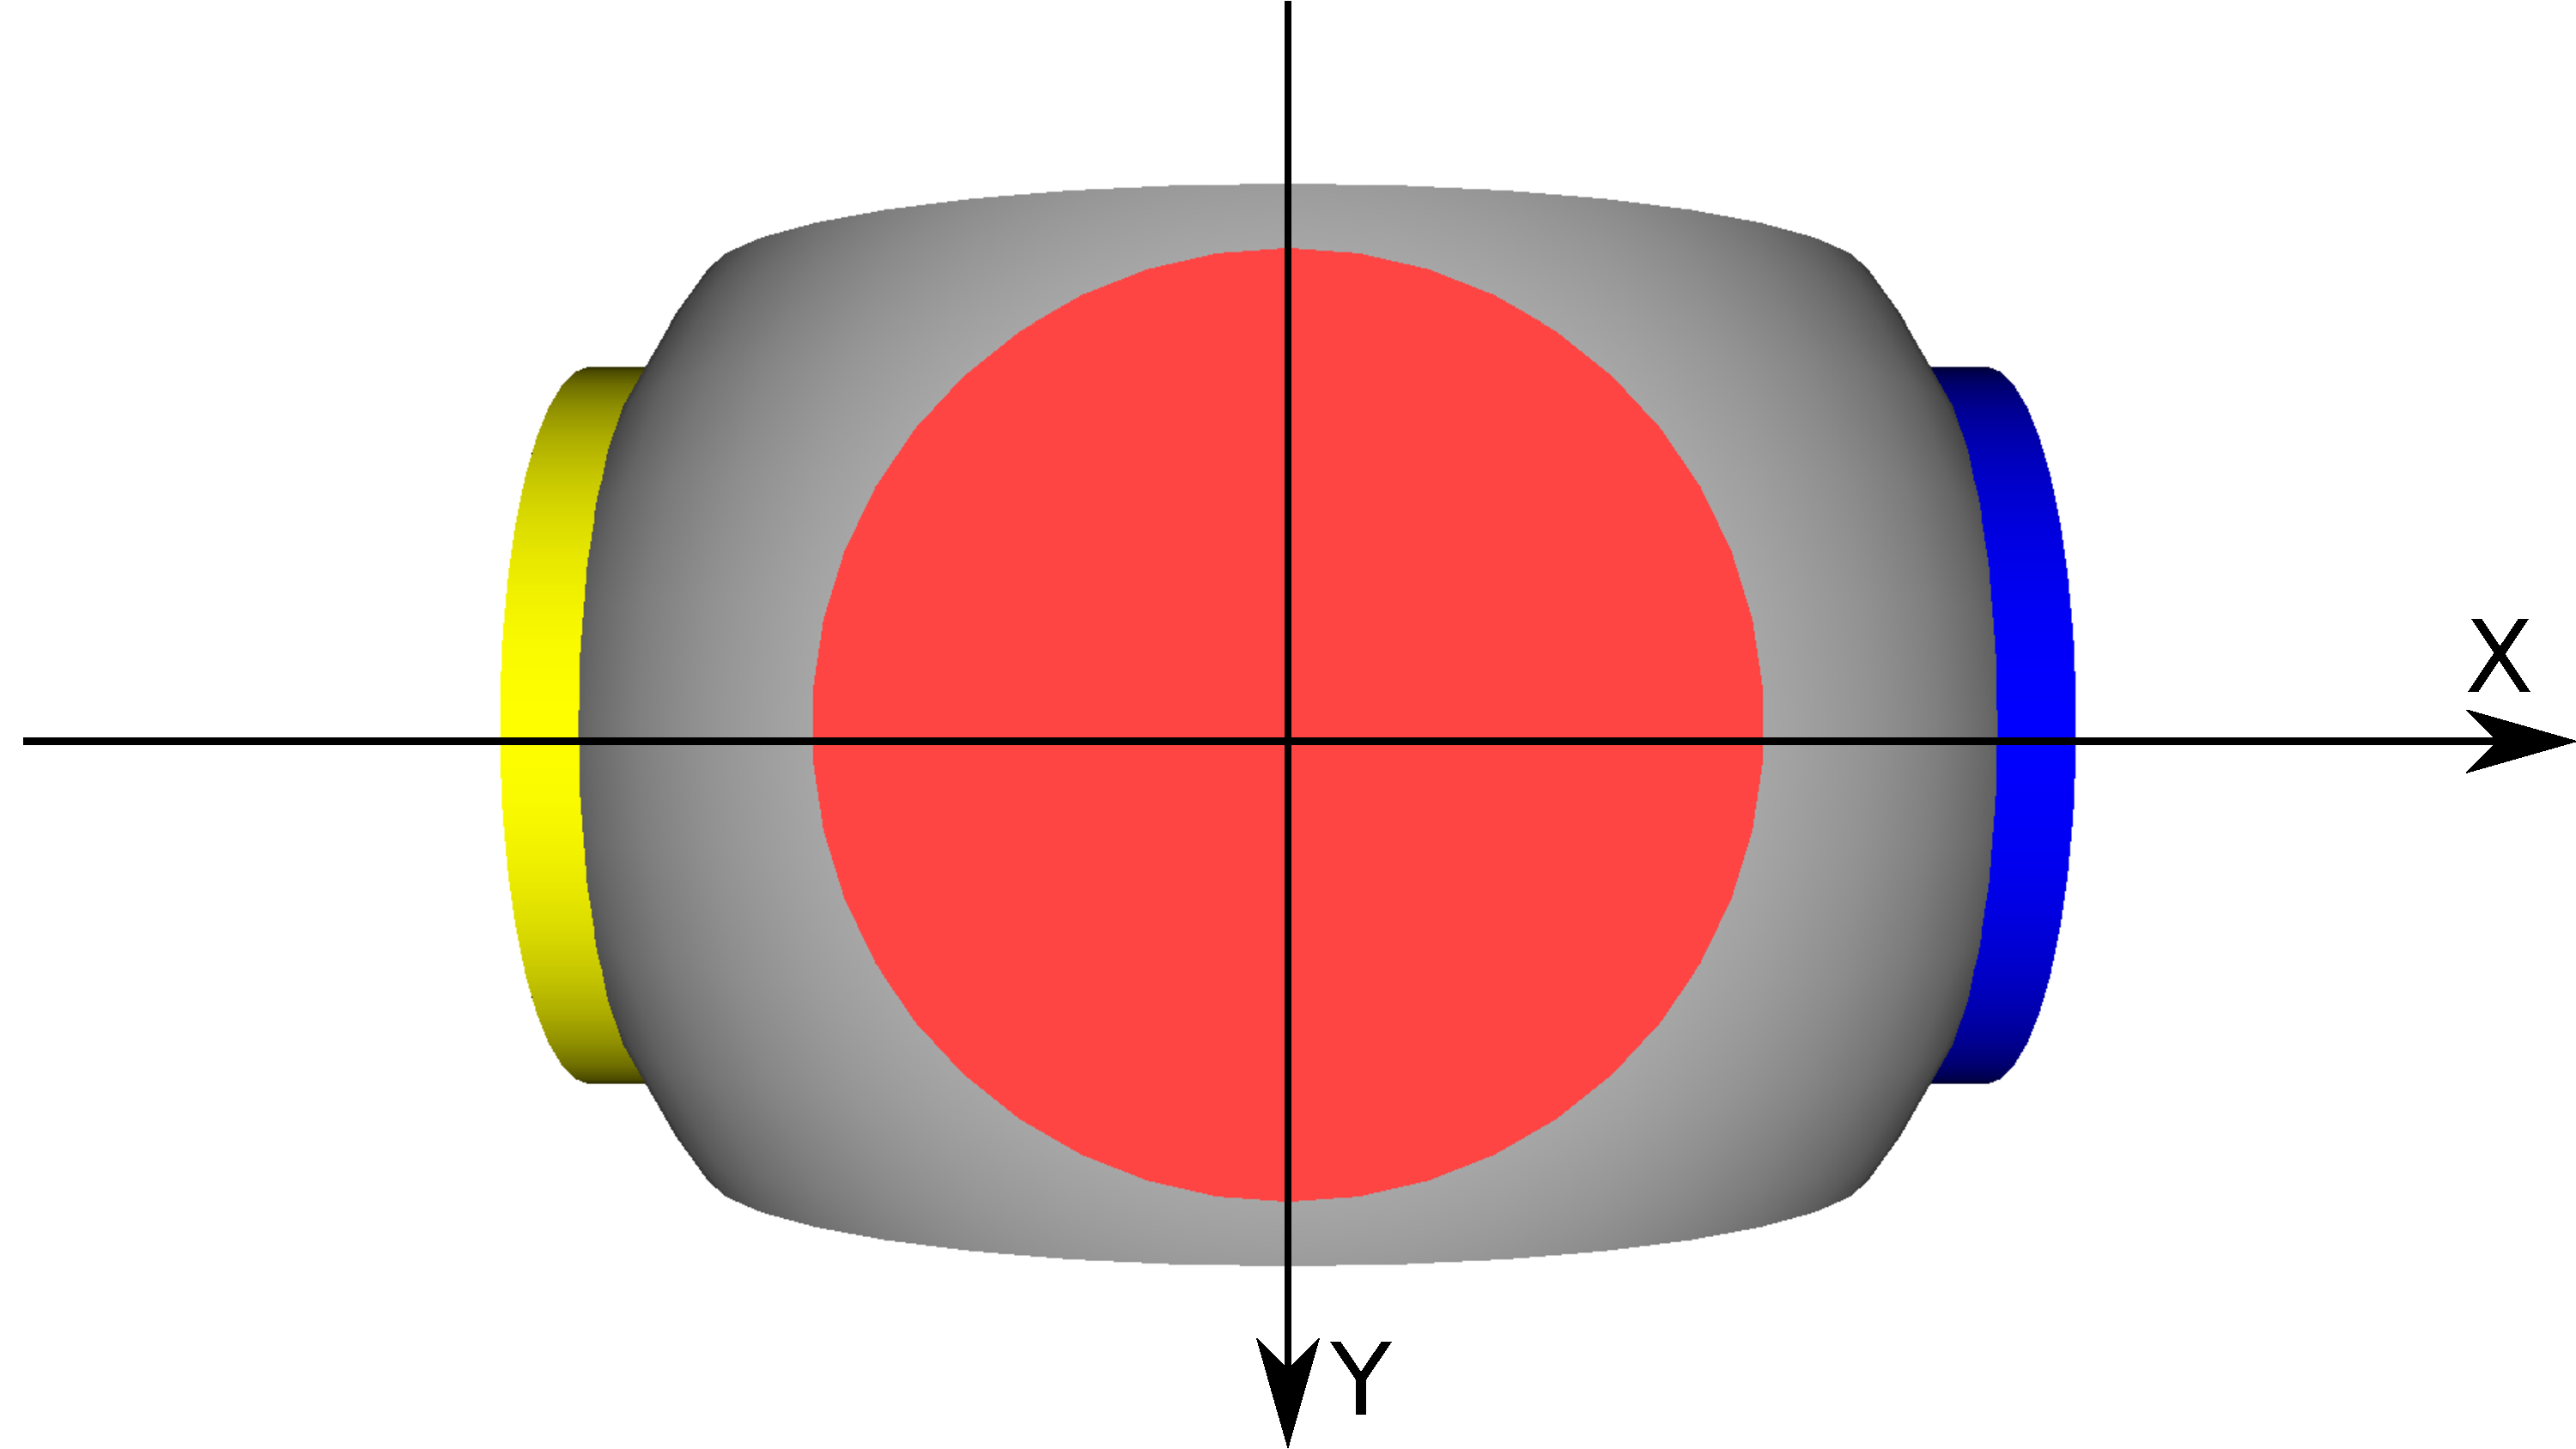
\includegraphics[width=\textwidth]{pictures/module_dock_identification_bottom.pdf}
        \caption[Pohľad zospodu]{Pohľad zospodu.}
    \end{subfigure}
    \caption[Definícia osí súradnicového systému]{Definícia osí súradnicového systému podľa polohy konektorov \textcolor{white}{\colorbox{modra}{$+X$}}, \colorbox{zlta}{$-X$} a \colorbox{cervena}{$-Z$} strany A~v~základnej pozícii. Ide o~pravotočivý súradnicový systém. }
    \label{fig:moduleAxis}
\end{figure}

Konceptuálne je súradnicový systém zavedený nasledovným spôsobom: Poloha strany A~modulu s~najnižším \textit{id} na začiatku konfigurácie definuje počiatok súradnicovej sústavy. Smer osí definuje následne strana B spomínaného modulu, ktorej súradnice sú $[0, 0, 1]$. Súradnice ostatných strán modulov sú dopočítané na základe ich polohy vzhľadom k~tomuto modulu. Podrobný popis výpočtov súradníc sa nachádza v~spomínanej diplomovej práci.  

Obrázok \ref{fig:moduleCoordinates} je ukážkou jednoduchej počiatočnej konfigurácie, kde sú moduly spojené stranami B. Teda strana A~žltého modulu je na súradniciach $[1, 0, 2]$. Os $y$ je jednoznačne definovaná, a to na základe pozícií konektorov (viď obrázok \ref{fig:moduleAxis}). Konektor $-Z$ strany A~modulu s~najnižším \textit{id} je orientovaný v~zápornom smere osi $z$ a konektory $-X$ a $+X$ na osi $x$ v~zápornom a kladnom smere v~tomto poradí. 

\begin{figure}[hbt!]
    \centering
    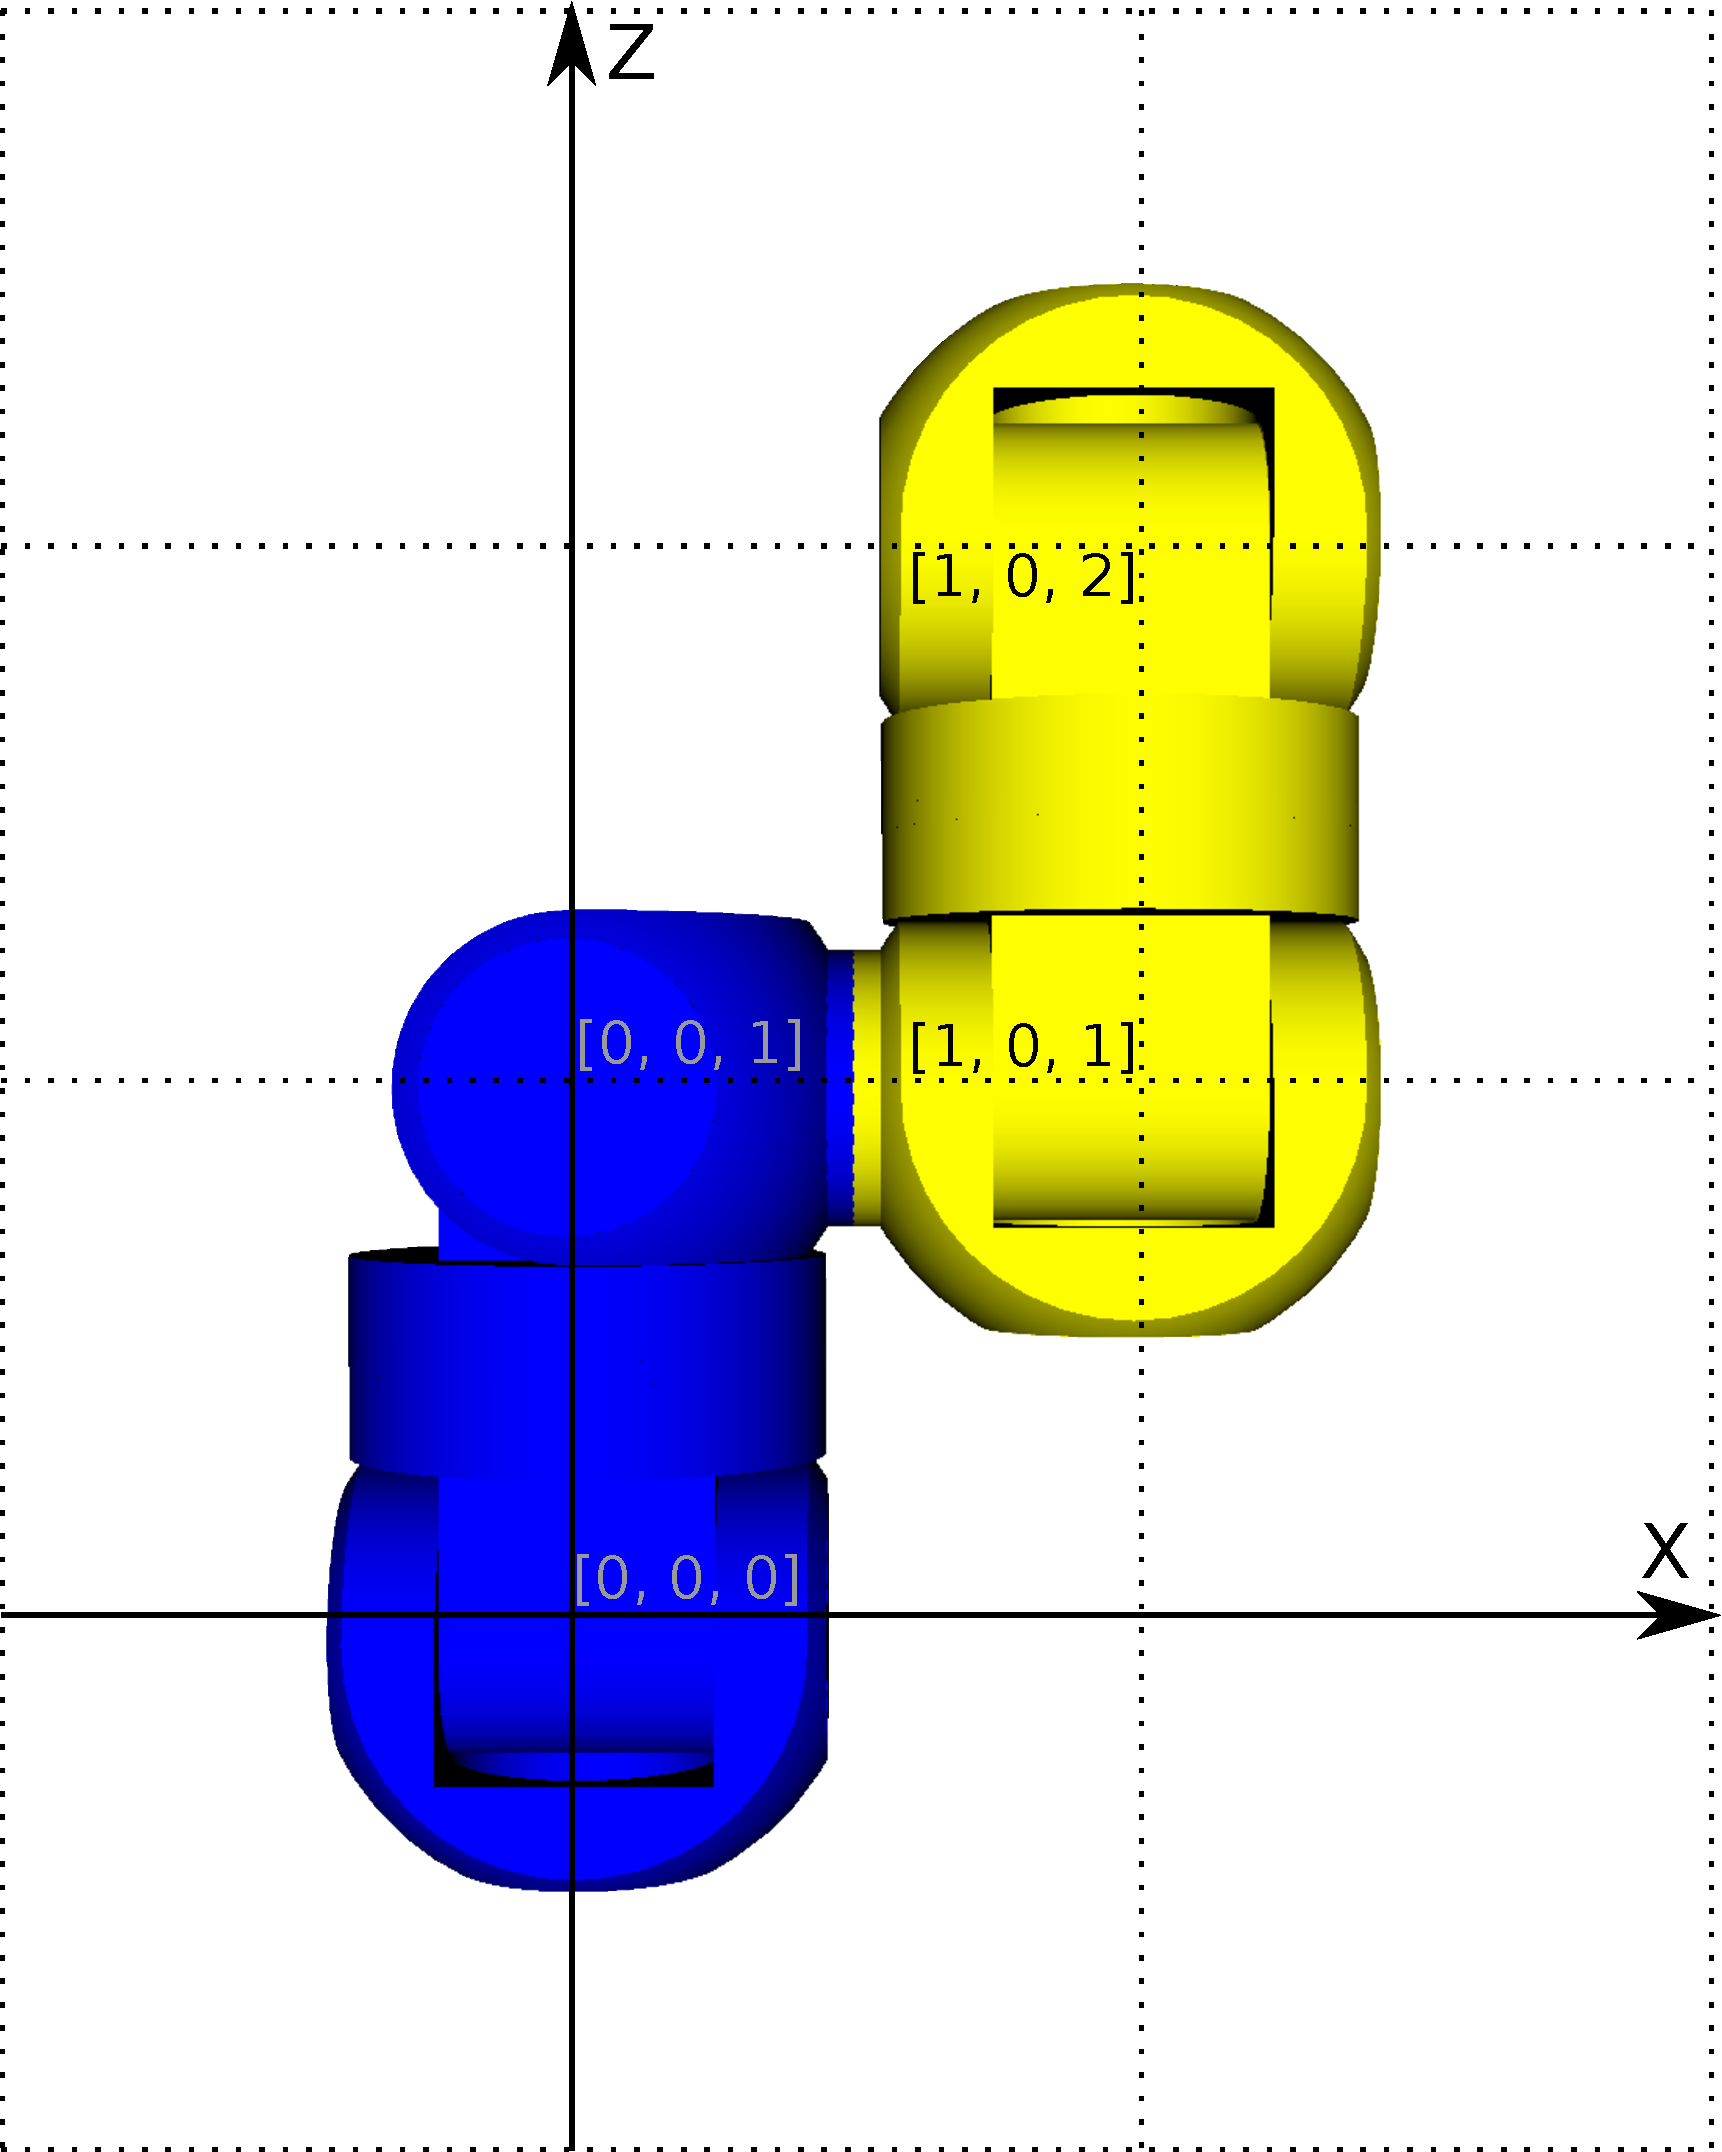
\includegraphics[width=0.6\textwidth]{pictures/module_coordinates.pdf}
    \caption[Ukážka súradnicového systému]{Príklad RoFIbota zasadeného do 3D súradnicového systému. Os $y$ smeruje od čitateľa. }
    \label{fig:moduleCoordinates}
\end{figure}

Celý súradnicový systém je zavedený podľa počiatočnej konfigurácie RoFIbota a počas rekonfigurácie ostáva fixovaný. Menia sa výhradne pozície modulov, ktoré si musia tieto vlastné súradnice prepočítavať. 

Algoritmus výpočtu súradníc v~spomínanej diplomovej práci je založený na znalosti celej konfigurácie RoFIbota. V~porovnaní s~tým algoritmus na rekonfiguráciu popísaný v~tejto kapitole znalosť celej konfigurácie RoFIbota nemá. Z~tohto dôvodu je z~algoritmu na výpočet súradníc použitá iba časť výpočtu matíc, z~ktorých sa dajú súradnice modulu získať. Zvyšok bol pozmenený nasledovným spôsobom: 

Modul s~najnižšou hodnotou \textit{id} pozná svoje súradnice (popísané vyššie). Následne každý modul, ktorý pozná svoje súradnice, vypočíta súradnice aj všetkým modulom, ktoré sú s~ním spojené hranou. Tento výpočet dokáže vykonať každý takýto modul, nakoľko pozná hodnoty svojich uhlov voľnosti, polohu konektorov a svoje vlastné súradnice. Následne pošle každému modulu, ktorý je s~ním spojený hranou, správu o~tom, aké má súradnice. Tento výpočet a rozposlanie správ sa dejú výhradne jednorázovo, nakoľko pri opakovaných výpočtoch a správach by došlo k~cykleniu správ. Proces popísaný v~tomto odseku sa opakuje, až kým nemá každý z~modulov znalosť o~svojich súradniciach. Algoritmus \ref{algorithm:coordinates} znázorňuje tento proces z~pohľadu jedného modulu -- ide o~program, ktorý má každý modul rovnaký. V~tomto algoritme je v~popise vstupu a výstupu stav algoritmu pred a po spustení. 

\begin{algorithm}
    \caption{Výpočet súradníc modulov RoFIbota. }
    \label{algorithm:coordinates}
    
    \DontPrintSemicolon
    \SetKwInOut{Input}{vstup}\SetKwInOut{Output}{výstup}
    \SetKwData{Id}{id}
    \Input{Konfigurácia RoFIbota bez znalosti zasadenia do~súradnicového systému.}
    \Output{Každý modul pozná svoje súradnice.}
    
    \If{\Id je najnižšie v~RoFIbotovi}{
        inicializuj počiatočné súradnice\;
    }
    zdieľaj a príjmi informácie o~znalosti súradníc\;
    \While{existuje modul, ktorý nepozná svoje súradnice}{
        \If{modul má známe súradnice {\bf and} tieto súradnice neboli zdieľané}{
            vypočítaj súradnice modulov, s~ktorými mám hranu\;
            pošli im ich súradnice\;
        }
        zdieľaj a príjmi informácie o~znalosti súradníc\;
    }
\end{algorithm}

Po tomto kroku má každý z~modulov uložené, aká je jeho aktuálna pozícia v~priestore, a teda môže prebiehať samotná rekonfigurácia. Základná myšlienka tejto rekonfigurácie je zachytená v~algoritme \ref{algorithm:algo2}. 

Slovne, rekonfigurácia začína výberom modulu (označme ho ako $\mathcal{M}$) a akcie, ktorú sa pokúsi vykonať. Pred vykonaním samotnej akcie je nutné, aby pomocou komunikácie s~ostatnými modulmi bolo zaručené, že danú akciu je možné bezpečne vykonať. Ak áno, tak sa vybraná akcia aj fyzicky vykoná, v~opačnom prípade sa nevykoná žiadna zmena konfigurácie. Tento postup sa opakuje, až kým nenastane jedna z~nasledujúcich podmienok: Prvá z~nich je, že každý modul je v~cieľovom stave, a druhá, že žiaden z~modulov už nemôže vykonať žiadnu akciu. 

\begin{algorithm}
    \caption{Distribuovaná rekonfigurácia. }
    \label{algorithm:algo2}
    
    \DontPrintSemicolon
    \SetKwInOut{Input}{vstup}\SetKwInOut{Output}{výstup}
    \SetKwData{Modul}{$\mathcal{M}$}
    \SetKwData{Action}{action}
    \Input{Každý modul je v~počiatočnom stave.}
    \Output{Každý modul je v~cieľovom stave alebo žiaden z~modulov už nedokáže vykonať žiadnu akciu.}
    
    \While{existuje modul, ktorý nie je v~cieľovom stave \\ \hspace{35}{\bf and} existuje modul, ktorý môže vykonať nejakú akciu}{
        \Modul $\leftarrow$ vyber modul\;
        \Action $\leftarrow$ vyber prípustnú akciu pre \Modul\;
        \If{\Modul môže vykonať akciu \Action}{
            \Modul vykoná akciu \Action\;
        }
    }
\end{algorithm}

Ostáva teda popísať spôsob výberu modulu, akcie daného modulu, a to, akým spôsobom sa testuje, že je možné danú akciu bezpečne vykonať. 

Implementovaný algoritmus využíva na výber modulu hodnoty unikátnych identifikátorov modulov. Moduly sú zoradené podľa hodnoty \textit{id} od najnižšieho po najvyšší a algoritmus vyberá moduly v~tomto poradí cyklicky. 

Akcie sa vyberajú tak, že sa preferujú rotácie pred prepojeniami. V~prípade, že má modul každý stupeň voľnosti správne natočený, tak nasledujú odpojenia a vytváranie nových hrán sa deje ako posledné v~poradí. Každá akcia je definovaná tak, že sa daný atribút zmení z~aktuálneho stavu priamo do cieľového stavu. Pri vytváraní prepojení to je vytváranie prepojenia výhradne s~modulmi, s~ktorými je modul prepojený v~cieľovom stave. Pri rotáciách ide o~analógiu, teda rotácia z~aktuálneho stavu uhla voľnosti do cieľového. Nakoľko žiaden modul nemá znalosť o~celej konfigurácii RoFIbota, tak na testovanie validity akcie je nutné použiť vzájomnú komunikáciu medzi modulmi. 

Validita rotácie akéhokoľvek stupňa voľnosti je definovaná výhradne tým, že nedôjde k~stretu žiadnych dvoch modulov. K~stretu dvoch modulov dôjde iba v~prípade, ak vzdialenosť stredov dotknutých strán modulov je menšia ako $1$. Je nutné otestovať, že počas celej rotácie nedôjde k~stretu žiadnych dvoch modulov. 

Zadefinujme si množinu $\mathcal{R}$ ako množinu modulov, ktorej sa počas rotácie zmenia súradnice (budú premiestnené). Zvyšné moduly budú patriť do množiny, ktorú si označíme ako $\mathcal{S}$. Vykonávaním rotácie nesmie dôjsť ku kolízii, ale tú stačí definovať iba medzi modulmi z~množiny $\mathcal{R}$ voči modulom z~množiny $\mathcal{S}$. Kolízie medzi modulmi z~množiny $\mathcal{S}$ nemôžu nastať, nakoľko sú všetky bez kolízií a ostávajú statické. V~množine $\mathcal{R}$ sa súradnice modulov menia, ale ich vzájomná poloha ostáva nezmenená, a teda ku kolíziám nemôže dôjsť. 

Testovanie na kolízie prebieha nasledovne: $\mathcal{M}$ (vybraný modul) si zistí pozície modulov v~množine $\mathcal{R}$ a na základe nich dokáže vypočítať, ako sa budú pohybovať stredy strán všetkých modulov v~$\mathcal{R}$. Tieto pozície pošle $\mathcal{M}$ všetkým modulom v~množine $\mathcal{S}$. Každý modul v~$\mathcal{S}$ dokáže na základe vlastnej polohy v~priestore určiť, či bude počas rotácie kolidovať s~niektorým z~modulov v~množine $\mathcal{R}$. Následne túto informáciu pošlú späť správou modulu $\mathcal{M}$. Z~pozbieraných údajov o~prípadných kolíziách dokáže $\mathcal{M}$ vyhodnotiť, či je rotácia bez kolízií. V~prípade, že ku kolízii nedôjde, tak vykoná rotáciu a modulom z~množiny $\mathcal{R}$ na záver rozpošle ich nové pozície v~priestore. 

V~porovnaní s~rotáciou je validita prepojenie modulov definovaná iba na dvoch moduloch, ktoré prepojenie tvoria. Označme si preto modul, ktorý sa podieľa na prepojení ako druhý, ako $\mathcal{M}'$ a hranu, ktorá je vybraná na spojenie/odpojenie, ako $\mathcal{E}$. 

Validita akcie odpojenia dvoch modulov je definovaná výhradne spojitosťou RoFIbota po vykonaní akcie. Tá je definovaná tak, že existuje fyzická cesta medzi každými dvomi modulmi. 

\begin{lemma}
\label{lemma:disconnection}
RoFIbot zostane spojitý po odpojení hrany $\mathcal{E}$ práve vtedy, keď existuje cesta medzi modulmi $\mathcal{M}$ a $\mathcal{M}'$ taká, že neobsahuje túto hranu. 
\end{lemma}

\begin{proof}
Dôkaz lemy \ref{lemma:disconnection} rozdelíme na dve časti. Najprv dokážeme, že ak existuje cesta s~uvedenými podmienkami, tak RoFIbot ostane spojitý. Vezmeme si ľubovoľné dva moduly a ukážeme, že medzi nimi existuje fyzická cesta aj po odpojení. Cesty medzi týmito dvomi modulmi sa dajú rozdeliť podľa toho, či obsahujú alebo neobsahujú hranu $\mathcal{E}$: 
\begin{itemize}
    \item obsahuje -- cestu z~pôvodnej konfigurácie je nutné pozmeniť, a to tak, že namiesto hrany $\mathcal{E}$ sa na toto miesto v~ceste vloží iná cesta medzi modulmi $\mathcal{M}$ a $\mathcal{M}'$, 
    \item neobsahuje -- cestu z~pôvodnej konfigurácie nie je nutné meniť, nakoľko všetky hrany budú naďalej existovať.
\end{itemize}

Ostáva ukázať, že ak je RoFIbot spojitý aj po rozpojení, tak v~pôvodnej konfigurácii existovala cesta z~$\mathcal{M}$ do $\mathcal{M}'$ neobsahujúca hranu $\mathcal{E}$. Keďže je konfigurácia po zmene spojitá, tak z~definície musí existovať cesta z~$\mathcal{M}$ do $\mathcal{M}'$ a zároveň neobsahuje hranu $\mathcal{E}$, lebo táto hrana sa v~zmenenej konfigurácii už nenachádza. Zároveň vieme, že sa konfigurácia inak nezmenila, takže táto cesta musí existovať aj v~pôvodnej konfigurácii, čím sme dokázali lemu. 

\end{proof}

Z~toho vyplýva, že stačí zistiť, či existuje cesta popísaná v~leme~\ref{lemma:disconnection}. Modulu $\mathcal{M}$ pošlú všetky moduly informáciu, s~akými ostatnými modulmi sú prepojené. Z~týchto údajov si modul $\mathcal{M}$ dokáže vytvoriť neorientovaný súvislý graf, kde každý modul je vrcholom a prepojenie medzi modulmi je hranou v~grafe. Zároveň je v~grafe povolené mať aj viacnásobné hrany medzi vrcholmi (maximálne však môžu existovať dve hrany medzi rovnakými vrcholmi). Hranu $\mathcal{E}$ do tohto grafu nepridávame (je to graf reprezentujúci konfiguráciu po odpojení). Následne pomocou \textit{BFS} z~vrcholu ekvivalentnému modulu $\mathcal{M}$ vyhľadáme cestu do vrcholu ekvivalentnému modulu $\mathcal{M}'$. Keďže tento výpočet prebieha nad konečným grafom, tak zaručene skončí. Odpojenie môžeme vykonať iba v~prípade, ak prehľadávanie do šírky nájde cestu do požadovaného vrcholu. 

Posledným typom akcie, ktorú môže vybraný modul vykonať, je pripojenie k~inému modulu. V~tomto prípade je pre validitu tejto akcie postačujúce, ak druhý modul spojenia (označme ho opäť ako $\mathcal{M}'$) je schopný zadaného prepojenia. Inak povedané, nachádza sa na správnych súradniciach a zároveň je správne natočený (správnym konektorom a jeho natočením voči konektoru modulu $\mathcal{M}$). Tieto súradnice a natočenia dokáže určiť modul $\mathcal{M}$ zo svojej polohy v~priestore a z~hodnôt uhlov voľnosti. Stačí teda, aby prebehla komunikácia medzi $\mathcal{M}$ a $\mathcal{M}'$, či $\mathcal{M}'$ má požadovanú polohu v~priestore a správne natočenie. Ak áno, prebehne spojenie modulov. 

% ------------------------------------------------------ 2 ------------------------------------------------------



% ------------------------------------------------------ 3 ------------------------------------------------------

\chapter{Implementácia rekonfiguračných algoritmov}
\label{sec:implementation}
Platforma RoFI je open-source projekt, ktorej súčasťou je aj knižnica RoFILib\footnote{\url{https://github.com/paradise-fi/RoFI/tree/master/RoFILib}}, ktorá sa zaoberá vývojom simulácií a vizualizácie. Implementačná časť tejto práce je súčasťou tejto knižnice. 

RoFILib je knižnica naprogramovaná v~jazyku C++. Táto knižnica poskytuje funkcie na simuláciu rekonfigurácie rôznymi algoritmami a z~rôznych pohľadov (centralizovaný a distribuovaný) na problém rekonfigurácie. V~súčasnej dobe sú to algoritmy navrhnuté v~rámci tejto práce a v~diplomovej práci \textit{Motion Planning for the RoFI Platform} \cite{vozarovaMasterThesis}.

Knižnica zároveň poskytuje možnosť vizualizácie konfigurácií a rekonfigurácií RoFIbotov. Vizualizér vznikol ako bakalárska práca \textit{Vizualizace pro robotickou platformu RoFI} \cite{nausovaBachelorThesis} a dokáže produkovať obrázky konfigurácie alebo videá rekonfigurácie. Väčšina obrázkov, ktoré sú súčasťou tejto práce a jej príloh, sú výstupom vizualizéru. 

\section{Návrh implementácie}
Problémy rekonfigurácie, ktoré riešia spomínané práce, majú jednotné vstupy a výstupy: Na vstupe sa nachádzajú dva súbory, ktoré popisujú počiatočnú a cieľovú konfiguráciu RoFIbota, ktorý sa má rekonfigurovať. Výstupom je súbor, ktorý obsahuje zoznam konfigurácií RoFIbota, ktoré vznikli po každom kroku rekonfigurácie. 

Podrobný popis vstupných a výstupných súborov sa nachádza v~diplomovej práci \textit{Motion Planning for the RoFI Platform} \cite{vozarovaMasterThesis} a ukážka v~prílohe \ref{sec:inOutFiles}. Keďže je definícia vstupov a výstupov pre rekonfiguračné problémy jednotná pre celú knižnicu RoFILib, tak je zaručená kompatibilita aj s~vizualizačným programom spomínanej knižnice. 

Vstupné a výstupné súbory obsahujú celú konfiguráciu RoFIbota, ktorej celková znalosť na vstupe simulácie ľubovoľného modulu nie je pre túto prácu možná. Preto je z~dôvodu kompatibility so zvyškom knižnice implementovaný aj preprocessing a postprocessing, ktorý obaľuje tu implementované algoritmy. 

Výpočet rekonfigurácie prebieha tak, že každý modul je samostatným procesom, ktorý dostane na vstup vstupné informácie (svoj počiatočný a cieľový stav). Spustené procesy si následne medzi sebou vymieňajú správy a na základe tejto komunikácie prebiehajú výpočty a validné akcie tak, aby sa každý modul rekonfiguroval z~počiatočného stavu do cieľového stavu. 

Aby bol výstup tejto práce plne kompatibilný s~vizualizérom knižnice RoFILib, tak sú jednotlivé vykonané akcie zapísané do logu (príklad logu je v~prílohe \ref{sec:log}). Na tých sa po skončení rekonfigurácie spustí postprocessing, ktorý vytvorí výstup kompatibilný so zvyškom knižnice. 

\section{Závislosti implementácie}
\label{sec:libraries}
Táto práca je zameraná na distribuované algoritmy a tie sú navrhnuté tak, aby každý modul RoFIbota fungoval ako samostatná entita. Komunikácia medzi entitami je možná výhradne pomocou správ a vo fyzických moduloch je uskutočnená pomocou protokolu MPI\footnote{Message Passing Interface}. Z~tohto dôvodu implementácia navrhnutých algoritmov využíva knižnicu OpenMPI \cite{openMPILibrary}, čo je open-source knižnica \cite{openMPIGit}, ktorá uľahčuje vývoj multiprocesových aplikácií v~distribuovanom prostredí. 

Keďže navrhnuté algoritmy majú simulovať výpočty rekonfigurácie fyzických modulov, tak je ich cieľom čo najviac sa priblížiť fyzickému modelu. To znamená, že algoritmy využívajú iba minimálnu sadu funkcií a možností knižnice OpenMPI, a to tie, ktoré je možné využiť vo fyzických moduloch, konkrétne v~implementácii sú využité nasledujúce súčasti knižnice OpenMPI: 
\begin{itemize}
    \item každý proces je unikátne identifikovaný, tzv. \textit{rank} procesu, 
    \item komunikácia medzi dvomi procesmi pomocou \textit{send} a \textit{recv} (jednosmerné posielanie dát) resp. \textit{sendrecv} (obojsmerné posielanie dát), 
    \item \textit{bcast} (broadcast): jednosmerné posielanie dát všetkým procesom, 
    \item \textit{gather}: všetky procesy posielajú dáta jednosmerne jednému procesu, 
    \item \textit{alltoall}: zdieľanie dát každý s~každým. 
\end{itemize}

Okrem toho bol návrh vytvorený tak, aby nepoužíval možnosti knižnice OpenMPI, ktoré sa nedajú využívať na fyzických moduloch. Príkladom tohto obmedzenia je nevyužívanie zdieľanej pamäte, nakoľko fyzické moduly žiadnu zdieľanú pamäť nemajú. 

Na praktické využitie knižnice na simuláciu rekonfigurácie a vizualizácie je nutné mať nainštalované nasledujúce knižnice: 
\begin{itemize}
    \item kompilátor C++, ktorý podporuje štandard aspoň C++17, 
    \item \texttt{cmake} verzie aspoň 3.10 -- v~prípade prekladu na základe súborov CMakeLists, 
    \item knižnica \texttt{Armadillo} -- slúži na prácu s~maticami a vektormi, ktoré sú potrebné na výpočty rekonfigurácie,  
    \item knižnice \texttt{VTK}, \texttt{FFmpeg} a grafický editor \texttt{Inkscape} -- závislosti vizualizačného nástroja, 
    \item knižnica \texttt{openMPI} -- na kompiláciu a spustenie distribuovaných algoritmov. 
\end{itemize}

 Návody na ich inštaláciu sa nachádzajú v~súbore \texttt{README.md}\footnote{\url{https://github.com/paradise-fi/RoFI/blob/master/RoFILib/README.md}} knižnice RoFILib. 

Knižnica OpenMPI spúšťa procesy tak, aby každý z~nich mal k~dispozícii samostatné jadro CPU, a to hlavne z~dôvodu, aby sa navzájom neovplyvňovali\footnote{\url{https://www.open-mpi.org/faq/?category=running\#oversubscribing}}. Preto je nutné, aby hardvérové vybavenie strojov, na ktorých bude bežať rekonfigurácia, malo aspoň toľko jadier CPU ako je počet modulov RoFIbota. 

\section{Použitie}
Výpočet algoritmov na rekonfiguráciu je možné spustiť buď ručne, alebo s~využitím pripraveného skriptu. V~prípade nevyužitia skriptu je nutné, aby vstup pre samotný algoritmus rekonfigurácie bol v~špecifickom tvare. Ten je zhodný s~formátom súborov, ktoré vytvára preprocessing.

\subsection{Preprocessing}
Preprocessing slúži na to, aby z~konfiguračných súborov kompatibilných s~knižnicou RoFILib vytvoril súbory pre distribuovanú rekonfiguráciu. Povinnými parametrami spustenia preprocessingu sú súbory s~počiatočnou a cieľovou konfiguráciou RoFIbota a adresár, kde môže vytvárať pomocné súbory. Medzi nepovinné parametre patria názvy súborov pre počet modulov a slovník. 

Výsledkom preprocessingu je príprava všetkých súborov potrebných na to, aby bolo možné využiť program na rekonfiguráciu a následný postprocessing: 
\begin{itemize}
    \item súbory \texttt{id.init} a \texttt{id.goal} (pre všetky \textit{id} modulov RoFIbota) -- obsahujú počiatočný, resp. cieľový stav modulu s~identifikátorom \textit{id} (príklad týchto súbor sa nachádza v~prílohe \ref{sec:algoInput}), 
    \item súbor \texttt{count} -- obsahuje počet modulov v~konfigurácii, resp. hodnotu $-1$, ak počet modulov v~počiatočnej a cieľovej konfigurácii nie je zhodný (teda ide o~nesprávne zadané vstupy), 
    \item súbor \texttt{dictionary} -- obsahuje slovník na preklad medzi pôvodnými identifikátormi modulov a identifikátormi využívanými pre rekonfiguráciu
\end{itemize}

Súbor \texttt{count} je použitý, aby bolo možné rýchlo zistiť, koľko procesov je nutné spustiť na rekonfiguráciu. Zavedenia slovníka je potrebné, nakoľko algoritmy navrhnuté v~tejto práci predpokladajú, že moduly majú hodnoty \textit{id} z~množiny $\interval[0, n - 1)$, kde $n$ je počet modulov RoFIbota.

Príklad spustenia preprocessingu, kde \mintinline{text}{init} a \mintinline{text}{goal} sú súbory obsahujúce počiatočnú a cieľovú konfiguráciu RoFIbota a \mintinline{text}{dir} je adresár, kde sa budú ukladať pomocné súbory, môže vyzerať takto:

\begin{minted}{bash}
  ./rofi-distribute-preprocessing -i init -g goal -d dir
\end{minted}.

\subsection{Rekonfigurácia}
Ak sú vstupné súbory pripravené v~tvare, ktorý vyžadujú algoritmy na rekonfiguráciu, tak je možné spustiť samotnú rekonfiguráciu. Samotný program vyžaduje adresár, v~ktorom sa nachádzajú vyššie popísané súbory s~počiatočným a cieľovým stavom každého modulu v~samostatnom súbore. Okrem toho vyžaduje aj výber algoritmu, ktorý má použiť na výpočet rekonfigurácie. 

V~prípade výberu algoritmu s~plnou znalosťou konfigurácie je možné zvoliť aj heuristiku pre výpočet algoritmu \textit{A*}. Podrobný popis princípov heuristík je uvedený v~diplomovej práci \textit{Motion Planning for the RoFI Platform} \cite{vozarovaMasterThesis}. 

Beh algoritmu rekonfigurácie prebieha tak, že sa spustí viacero procesov naraz. Toto umožňuje knižnica OpenMPI, a to pomocou príkazu \mintinline{bash}{mpiexec} s~vhodnými prepínačmi: Je nutné nastaviť počet procesov pomocou prepínača \mintinline{bash}{-np}. Zároveň je možné spúšťať tieto procesy plne distribuovane, teda na viacerých strojoch naraz, a tie sa špecifikujú prepínačom \mintinline{bash}{--hostfile} s~názvom súboru, ktorý obsahuje zoznam hostiteľských strojov\footnote{Popis formátu hostiteľských strojov sa nachádza na \url{https://www.open-mpi.org/faq/?category=running\#mpirun-hostfile}.}. 

Nech \mintinline{text}{host-file} je súbor so špecifikovanými hostiteľskými strojmi a \mintinline{text}{dir} je adresár, v~ktorom sú súbory s~počiatočnými a cieľovými stavmi modulov. Príkaz na spustenie napríklad algoritmu s~plnou znalosťou konfigurácie RoFIbota na rekonfiguráciu $4$ modulov s~triviálnou heuristikou je: 
\begin{minted}{bash}
  mpiexec --hostfile host-file -np 4 \
    ./distribute/rofi-distribute -d dir -a full -e trivial
\end{minted}.

Výstup algoritmu je vypísaný na štandardný výstup. Jeho formát je nasledovný: Na úplnom začiatku je uvedená počiatočná konfigurácia RoFIbota tak, že každý riadok konfigurácie obsahuje prefix $0$. Nakoľko program nemá plnú znalosť konfigurácie, tak ju vytvorí tak, že každý modul vypíše svoj stav. Nasledujúce riadky obsahujú vykonané akcie, pričom ich poradie nemusí byť zhodné s~poradím, v~akom sa dané akcie vykonávali. Preto má každá akcia na začiatku svojho zápisu kladný celočíselný prefix, ktorý hovorí o~poradovom čísle kroku, v~ktorom sa daná akcia vykonala. Zároveň sa predpokladá, že výstup obsahuje všetky poradové čísla krokov (teda v~každom kroku sa vykoná vždy aspoň jedna akcia). Ak je použitý druhý algoritmus a nastane prípad, že rekonfigurácia už nemôže pokračovať, ale aspoň jeden modul nie je v~cieľovej konfigurácii, tak na konci výstupu je poznámka o~skutočnosti, že nejde o~cieľový stav RoFIbota. 

\subsection{Postprocessing}
Tento výstup však nie je kompatibilný so zvyšnými časťami knižnice RoFILib. Na to slúži pripravený postprocessing, ktorý dokáže transformovať vzniknutý formát súboru z~navrhnutých algoritmov do formátu kompatibilného s~knižnicou. 

Cieľom postprocessingu je vytvoriť súbor, ktorý obsahuje postupnosť konfigurácií rekonfigurácie RoFIbota, pričom na vstupe má súbor, kde sú časovými známkami označené počiatočná konfigurácia a akcie, ktoré sa na danej konfigurácii majú vykonávať. Teda postprocessing vezme súbor s~akciami a postupne ich podľa časových známok aplikuje na počiatočnú konfiguráciu. Zároveň aj premenuje identifikátory modulov podľa zadaného slovníka, ktorý bol napríklad vytvorený ako produkt preprocessingu. 

Nech \mintinline{text}{file} je súbor obsahujúci hodnoty, ktoré sú zhodné s~výstupom rekonfiguračného algoritmu a \mintinline{text}{dictionary} je súbor, v~ktorom je uvedený preklad unikátnych identifikátorov modulov. Postprocessing môže byť spustený napríklad takýmto príkazom: 
\begin{minted}{bash}
  ./rofi-distribute-postprocessing -i file -t dictionary
\end{minted}

Toto je kompletný popis využitia časti \textit{rofi-distribute} knižnice RoFILib, ktorá vznikla ako implementačná časť tejto bakalárskej práce. Nakoľko je z~dôvodu kompatibility s~knižnicou nutné spúšťať preprocessing a postprocessing, tak je pripravený aj skript \textt{distribute.sh}, ktorý túto sekvenciu spúšťania všetkých častí vykoná automaticky. 

Zoznam a podrobný popis všetkých prepínačov, ktoré sa využívajú v~jednotlivých častiach knižnice a skripte, sa nachádzajú v~\texttt{README.md}\footnote{\url{https://github.com/paradise-fi/RoFI/blob/master/RoFILib/README.md}} resp. časť, ktorá sa týka algoritmov implementovaných v~tejto práci sa nachádza v~prílohe \ref{sec:readme}. 

% ------------------------------------------------------ 3 ------------------------------------------------------




% ------------------------------------------------------ 4 ------------------------------------------------------
\chapter{Experimentálne vyhodnotenie}
Oba navrhnuté a implementované algoritmy boli otestované na vzorových vstupoch. Vyhodnotenie spočíva v~porovnávaní časov, ktoré boli nutné na ich výpočet, schopnosti nájsť riešenie a zároveň aj porovnaní dĺžok nájdených rekonfiguračných postupností. 

\section{Testovacie rekonfigurácie}
Vzorové vstupy vznikli generátorom konfigurácií\footnote{\url{https://github.com/paradise-fi/RoFI/tree/master/RoFILib/generate}}, ktorý patrí do knižnice RoFILib. 

Testované vstupy sú vybrané tak, že ich počiatočná konfigurácia je vygenerovaná náhodne s~tým, že má vopred určený počet modulov. Tie sú vybrané tak, aby pokryli rôzne veľkosť RoFIbotov od malých konfigurácií s~$2$, $3$ alebo $5$ modulmi po veľké konfigurácie s~$15$, $50$ a $80$ modulmi. Vybrané počiatočné konfigurácie sú zobrazené na obrázku~\ref{fig:rofibotExamples}. 

Cieľová konfigurácia je vygenerovaná tak, že generátor vygeneruje zadaný počet validných krokov a tie sa postupne aplikujú na počiatočnú konfiguráciu. Tento prístup zaručuje existenciu rekonfiguračnej postupnosti. Vzorové vstupy sú generované na rekonfigurácie dĺžok $5$, $10$, $20$, $30$ a $50$ krokov. 

Každý vstup má na základe týchto údajov aj určené označenie. Názvy vstupných súborov majú nasledujúci formát:

\texttt{<počet modulov>-<počet krokov>-\{init,goal\}.in}. 

Napríklad súbor s~popisom konfigurácie na obrázku \ref{fig:3-10-init} sa nazýva \textit{3-10-init.in}, nakoľko ide o~konfiguráciu s~$3$ modulmi, ktorá bola generovaná na rekonfiguráciu s~$10$ krokmi. 

\begin{figure}[hbt!]
    \centering
    \begin{subfigure}[b]{0.47\textwidth}
        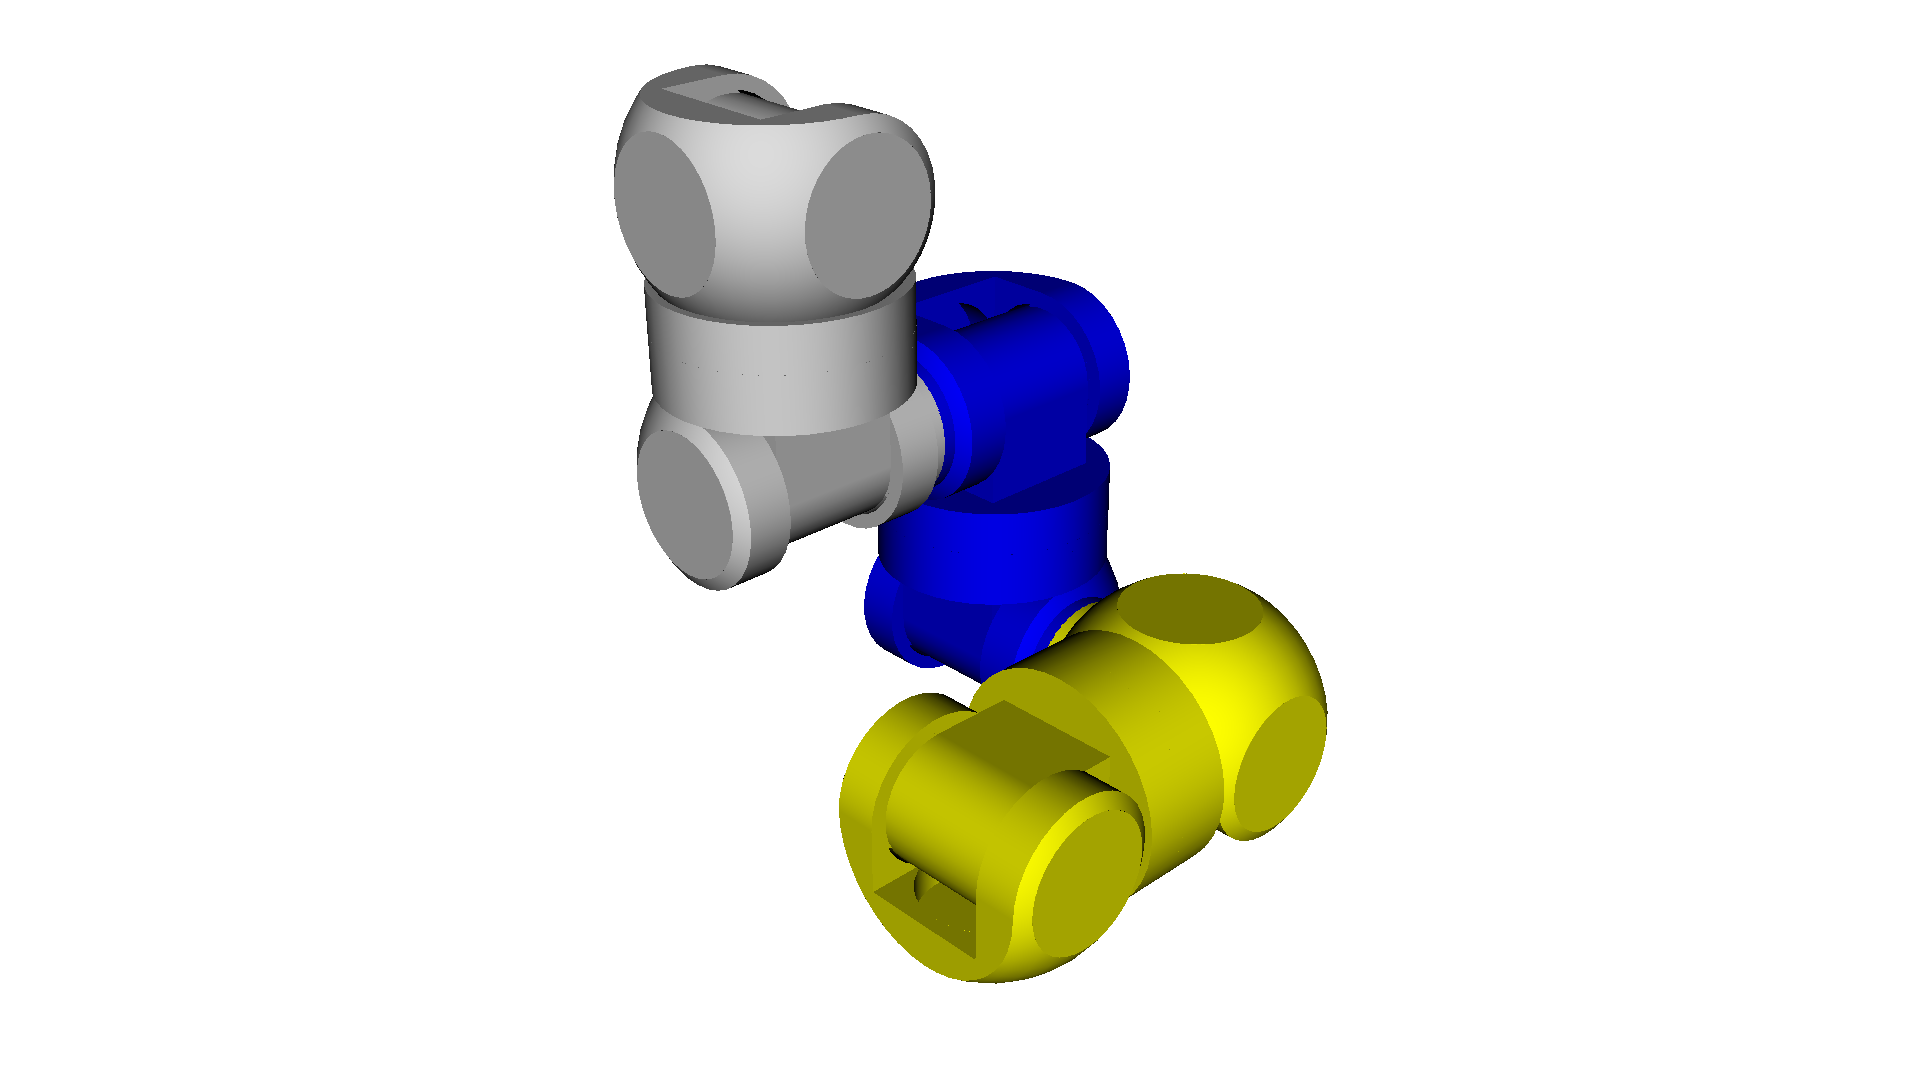
\includegraphics[width=\textwidth]{pictures/3-10-init.png}
        \caption[3-10-init]{Vstupná konfigurácia $3$-$10$.}
        \label{fig:3-10-init}
    \end{subfigure}
    \begin{subfigure}[b]{0.47\textwidth}
        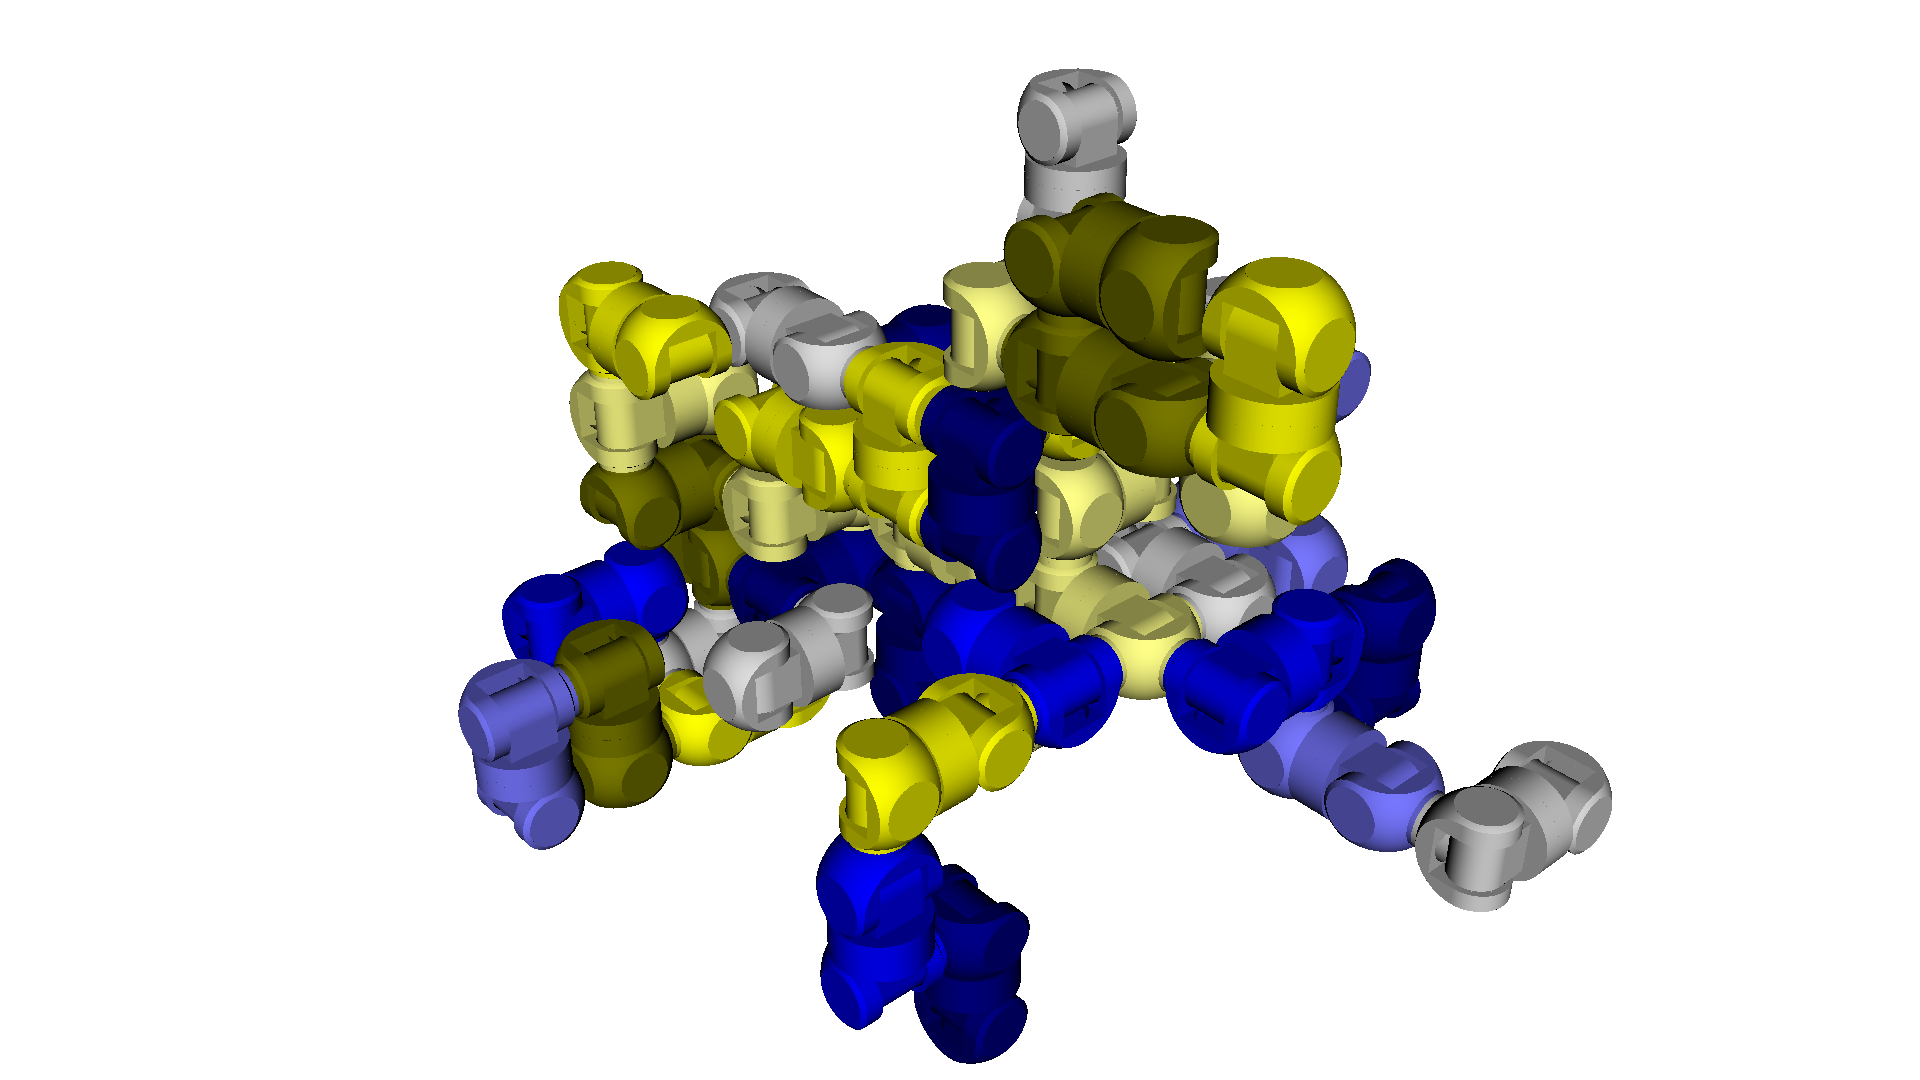
\includegraphics[width=\textwidth]{pictures/50-5-init.png}
        \caption[50-5-init]{Vstupná konfigurácia $50$-$5$.}
    \end{subfigure}
    \caption[Ukážkové vstupné konfigurácie]{Ukážka vstupných konfigurácií vygenerovaných náhodne. }
    \label{fig:rofibotExamples}
\end{figure}

\newcommand{\comment}[1]{}
\comment{
Okrem náhodne generovaných vstupov boli skúšané aj ručne vytvorené vstupy, kde nie je nutne zaručená existencia rekonfigurácie. Niektoré príklady vizualizuje obrázok \ref{fig:rotationExampleByHand}. }

Nakoľko algoritmy navrhnuté v~tejto práci potrebujú dostatočný počet jadier procesorov, tak boli vstupy spúšťané na potrebnom počte strojov z~$22$ hardvérovo zhodne vybavených strojov. Každý z~nich má štvorjadrový procesor Intel Xeon 5130 o~takte $2.00$\,GHz a $16$\,GB RAM. 

\section{Evaluácia výsledkov na testovacích rekonfiguráciách}
Všetky namerané hodnoty sa nachádzajú v~tabuľkách v~prílohe \ref{tab:tables}. Hodnoty vyznačené \colorbox{table-green}{zelenou} predstavujú najlepší čas výpočtu rekonfigurácie v~porovnaní s~inými heuristikami a v~prípade rovnosti časov ide o~najkratšiu výslednú rekonfiguračnú postupnosť. 

V~celej evaluácii budeme používať značenie testov \textit{X-Y}, kde \textit{X} je počet modulov v~konfigurácii a \textit{Y} je počet krokov rekonfigurácie, ktoré boli vykonané, aby vznikla cieľová konfigurácia RoFIbota. 

V~tabuľke \ref{tab:all} je použitý vždy najlepší výsledok merania pre daný vstup a algoritmus. To znamená, že uvedené časy a dĺžky výsledných postupností nemuseli vzniknúť pomocou rovnakej heuristiky. Nakoľko algoritmus s~čiastočnou znalosťou konfigurácie vždy nenašiel riešenie, tak sú v~tabuľke zahrnuté iba namerané hodnoty tých vstupov, kde sa podarilo nájsť celú rekonfiguračnú postupnosť. 

\begin{table}[hp!]
\centering
\begin{tabular}{c|cc|cc|cc}
\multirow{2}{*}{} & \multicolumn{2}{c|}{full} & \multicolumn{2}{c|}{\textit{A*}} & \multicolumn{2}{c}{partial} \\
 & čas & dĺžka & čas & dĺžka & čas & dĺžka \\ \hline
2-5  & 00:02 & \cellcolor{table-green}4  & 00:00 & 5  & \cellcolor{table-green}00:02 & 5 \\
2-10  & 00:02 & \cellcolor{table-green}2  & 00:00 & 6  & \cellcolor{table-green}00:02 & 5 \\
2-20  & \cellcolor{table-green}00:04 & \cellcolor{table-green}4  & 00:01 & 14  & X & X \\
2-30  & \cellcolor{table-green}00:02 & \cellcolor{table-green}6  & 00:00 & 13  & X & X \\
2-50  & \cellcolor{table-green}00:02 & \cellcolor{table-green}4  & 00:00 & 14  & X & X \\ \hline
3-5  & 00:02 & \cellcolor{table-green}2  & 00:00 & 6  & \cellcolor{table-green}00:02 & 5 \\
3-10  & 00:02 & \cellcolor{table-green}2  & 00:00 & 7  & \cellcolor{table-green}00:02 & 5 \\
3-20  & \cellcolor{table-green}00:02 & \cellcolor{table-green}4  & 00:00 & 11  & X & X \\
3-30  & 00:02 & \cellcolor{table-green}2  & 00:00 & 11  & \cellcolor{table-green}00:02 & 9 \\
3-50  & \cellcolor{table-green}00:03 & \cellcolor{table-green}5  & 00:00 & 15  & X & X \\ \hline
5-5  & 00:02 & \cellcolor{table-green}3  & 00:00 & 8  & \cellcolor{table-green}00:02 & 8 \\
5-10  & \cellcolor{table-green}00:07 & \cellcolor{table-green}6  & 00:04 & 15  & X & X \\
5-20  & \cellcolor{table-green}01:50 & \cellcolor{table-green}6 & 01:16 & 17  & X & X \\
5-30  & \cellcolor{table-green}00:03 & \cellcolor{table-green}4  & 00:01 & 15  & X & X \\
5-50  & -- & --  & 28:14 & 53  & X & X \\ \hline
10-5  & 00:02 & \cellcolor{table-green}2  & 00:00 & 5  & \cellcolor{table-green}00:02 & 5 \\
10-10  & \cellcolor{table-green}00:03 & \cellcolor{table-green}3  & 00:00 & 11  & X & X \\
10-20  & 05:16 & \cellcolor{table-green}4  & 05:11 & 17  & \cellcolor{table-green}00:02 & 16 \\
10-30  & \cellcolor{table-green}00:22 & \cellcolor{table-green}11  & 00:07 & 35  & X & X \\
10-50  & -- & --  & -- & --  & X & X \\ \hline
15-5  & \cellcolor{table-green}00:16 & \cellcolor{table-green}4  & 00:01 & 9  & X & X  \\
15-10  & \cellcolor{table-green}00:22 & \cellcolor{table-green}5  & 00:04 & 17  & X & X \\
15-20  & -- & --  & -- & --  & X & X \\
15-30  & -- & --  & -- & --  & X & X \\
15-50  & -- & --  & -- & --  & X & X \\ \hline
50-5  & 00:17 & \cellcolor{table-green}2  & 00:17 & 6  & \cellcolor{table-green}00:03 & 6 \\ \hline
80-5  & 00:28 & \cellcolor{table-green}2  & 00:26 & 6  & \cellcolor{table-green}00:04 & 6 \\
\end{tabular}%
\caption{V~prvom stĺpci tabuľky sa nachádza označenie testu. Ostatné stĺpce znázorňujú výsledky v~dĺžke výpočtu rekonfigurácie (vo formáte \textit{minúty:sekundy}) a dĺžke výslednej rekonfiguračnej postupnosti. \\ \colorbox{table-green}{Zelenou} je vyznačený čas/dĺžka, ktoré boli rýchlejšie/kratšie v~porovnaní algoritmov s~plnou resp. čiastočnou znalosťou konfigurácie. Označenie \mbox{\uv{--}} predstavuje výpočet, ktorý neskončil do vypršania timeoutu 30 minút. Označenie \uv{\textit{X}} prestavuje, že algoritmus neskončil v~cieľovej konfigurácii. }
\label{tab:all}
\end{table}

V~prvom rade je nutné porovnať dĺžky výpočtov a dĺžky výslednej rekonfiguračnej postupnosti medzi algoritmom s~úplnou znalosťou konfigurácie a algoritmom \textit{A*}. Algoritmus s~úplnou znalosťou využíva algoritmus \textit{A*} hneď po zistení celkovej konfigurácie RoFIbota, čo znamená, že čas potrebný na výpočet algoritmu s~plnou znalosťou je nutne väčší ako pre algoritmus \textit{A*}. 

Zároveň platí, že je nutné brať ohľad na označenie modulov v~RoFIbotovi. Na základe tabuliek \ref{tab:astar-orig} a \ref{tab:astar-renamed} je tento rozdiel značný už pri RoFIbotoch s~$5$ modulmi, kde napríklad vstup \textit{5-50} s~heuristikou dMatrix trvá v~pôvodnom značení identifikátorov iba niečo viac ako $2$ minúty, ale po zmene značenia preprocessingom je nutné mať na rekonfiguráciu $28$ minút. Opačný prípad nastáva napríklad pri vstupe \textit{80-5} s~heuristikou dMatrix. 

Výsledkom porovnania algoritmu s~plnou znalosťou konfigurácie a algoritmu \textit{A*} v~najkratších časoch rekonfigurácie a dĺžkach výslednej rekonfiguračnej postupnosti je, že čas sa nepravidelne zvyšuje (od zanedbateľných stotín percenta až po trojnásobok pôvodného výpočtu), ale dĺžka cesty sa vo väčšine prípadov skrátila na tretinu pôvodnej dĺžky. Nakoľko je možné optimalizáciu tohto algoritmu v~akomkoľvek bode zastaviť, tak je tento algoritmus minimálne efektívny z~pohľadu toho, že dokáže v~niektorých prípadoch za krátke navýšenie výpočtového času efektívne skrátiť dĺžku rekonfiguračnej postupnosti. 

Algoritmus s~čiastočnou znalosťou konfigurácie dokáže nájsť výhradne tzv. triviálne riešenie. Pod týmto pojmom je možné predstaviť si to, že po každom kroku rekonfigurácie niektorý z~modulov zmení buď jeden zo svojich stupňov voľnosti alebo niektorú hranu do cieľového stavu. Teda ak algoritmus s~čiastočnou znalosťou rekonfigurácie nájde riešenie, tak je jednoznačne najkratšie možné z~pohľadu počtu vykonaných akcii (nie nutne počtu krokov). 

Zároveň je tento algoritmus navrhnutý tak, aby jeho beh netrval dlho, čo dokazujú aj namerané hodnoty. Teda, ak tento algoritmus našiel riešenie, tak bol výpočet rýchlejší ako algoritmus s~úplnou znalosťou (pri väčšom počte modulov). 

Namerané hodnoty ukazujú, že je vhodné použiť algoritmus s~čiastočnou znalosťou konfigurácie na rýchle prehľadanie priestoru, či neexistuje triviálne riešenie, ktoré z~nameraných hodnôt minimálne u~krátkych rekonfiguračných postupností existuje. Algoritmus s~úplnou znalosťou konfigurácie je zase vhodné využívať pri optimalizácii už nájdeného riešenie, pričom je možné optimalizáciu v~akomkoľvek čase pozastaviť a pokračovať už samotnou rekonfiguráciou. 


% ------------------------------------------------------ 4 ------------------------------------------------------





% ------------------------------------------------------ 5 ------------------------------------------------------
\chapter{Záver}
Táto práca stručne prezentovala robotickú platformu RoFI, a to predovšetkým popis modulu, matematický model popisujúci stav modulu a popis konfigurácie a rekonfigurácie RoFIbota. V~práci sa taktiež nachádza popis mnou navrhnutých dvoch distribuovaných algoritmov na rekonfiguráciu, dôkazy ich korektnosti a ich pozitívne, ale aj negatívne vlastnosti. Súčasťou práce je aj implementácia navrhnutých algoritmov a v~práci sa nachádza aj popis použitia implementácie. 

Navrhnuté a implementované algoritmy boli otestované a vzájomne porovnané na vzorových vstupoch rôznych veľkostí RoFIbotov či dĺžke rekonfigurácií. V~prípade algoritmu s~úplnou znalosťou konfigurácie bolo zistené, že celkový čas rekonfigurácie síce prebiehal na vzorových vstupoch v~priemere trikrát dlhšie ako samotné centralizované plánovanie rekonfigurácie, ale počet krokov rekonfigurácie sa podarilo znížiť takmer na pätinu. To je samozrejme v~prípade fyzických modulov prijateľný čas, nakoľko fyzická zmena trvá priemerne dlhšie ako samotné výpočty optimalizácie postupnosti rekonfigurácie. 

Druhý algoritmus síce v~niektorých prípadoch nenájde žiadne riešenie, ale ak už riešenie nájde, tak je zaručene najkratšie možné. Zároveň je výpočet druhého algoritmu v~porovnaní s~prvým významne kratší aj na veľkých vstupoch, takže je vhodné využiť ho minimálne ako vhodnú heuristiku pred spustením iného algoritmu na rekonfiguráciu. 

\section{Možnosti rozšírenia práce}
\label{sec:future}
V~práci je popísaný aktuálny stav algoritmov na distribuovanú rekonfiguráciu. Algoritmy sú navrhnuté tak, aby sa dali jednoducho modifikovať a optimalizovať, čo umožní jednoduchšie zapracovanie napríklad nižšie popísaných zmien. 

V~prípade algoritmu s~plnou znalosťou konfigurácie ide hlavne o~samotný výpočet postupnosti krokov rekonfigurácie a jej optimalizáciu. V~súčasnej dobe je tento algoritmus implementovaný tak, že každý modul počíta rovnaké hodnoty a na základe nich sa následne vykonáva fyzická rekonfigurácia. Jedným z~návrhov na zlepšenie tohto algoritmu je, že každý z~modulov môže počítať postupnosť krokov rôznymi algoritmami a inými heuristikami. Išlo by v~podstate o~prístup, ktorý bol využitý pri evaluácii tohto algoritmu, kde sa vždy vyberie najrýchlejší výsledok, resp. z~najrýchlejších výsledkov ten najkratší. 

Druhou časťou vhodnou na budúce zlepšenie je samotná optimalizácia krokov. Aktuálny prístup optimalizácie krokov je greedy, a teda nemusí vždy nájsť optimálne riešenie. Ďalším zlepšením je teda riešenie optimalizácie iným spôsobom, napríklad vzájomnou komunikáciou modulov, ktoré sa dohodnú, či je lepšie pokračovať v~hľadaní optimálnej postupnosti alebo bude tento výpočet trvať dlho a prejdú na samotnú rekonfiguráciu za cenu dlhšej postupnosti krokov. Alternatívne môžeme využiť fakt, že RoFIbot tvorí distribuovaný systém, a počítať optimalizácie rôznymi prístupmi. 

V~prípade druhého algoritmu (bez znalosti celej konfigurácie) je častí na zlepšovanie oveľa viac. Navrhnutý algoritmus totiž nedokáže vždy s~istotou nájsť triviálne riešenie, ak existuje, a teda jednou alternatívou zlepšovania tohto algoritmu je vyvinutie lepšieho výberu modulu, ktorý bude vykonávať akciu. S~tým súvisí aj vylepšenie heuristiky výberu akcie, ktorú ma vyberaný modul vykonať. 

Predchádzajúce zlepšenia však neriešia problém toho, že nie každá rekonfigurácia je nutne triviálna. Preto jedným z~riešením takýchto prípadov je upraviť konfiguráciu pred spustením samotnej rekonfigurácie, čo s~ňou umožní lepšiu manipuláciu. Príkladom môže byť vytvorenie stromu, ktorý umožní rotáciu viacerým modulom. Ďalším krokom k~zlepšeniu tohto algoritmu je vývoj heuristiky, ktorá zistí, kedy je vhodné vykonať akciu, ktorá síce neposúva konfiguráciu priamo k~cieľovej konfigurácii, ale umožní tým ďalšie akcie, ktoré môžu viesť k~cieľovej konfigurácii. 

V~prípade oboch algoritmov je možné uvažovať o~optimalizácii premenovania uzlov tak, aby bol výpočet centralizovaného riešenia rekonfigurácie vypočítaný za čo najkratší čas s~minimálnou dĺžkou postupnosti.

% ------------------------------------------------------ 5 ------------------------------------------------------

\cleardoublepage
\appendix
\chapter{Príklady vstupných a výstupných súborov}
\label{sec:inOutFiles}
\section{Vstupné súbory}
\subsection{Počiatočná konfigurácia}
M 9 90 90 90 \\
M 10 90 0 90 \\
M 5 -90 -90 -90 \\
E 9 A~+X W +X A~10 \\
E 5 A~+X W +X B 9

\subsection{Cieľová konfigurácia}
M 9 -90 90 0 \\
M 10 90 0 0 \\
M 5 -90 0 0 \\
E 9 B -X N -Z B 10 \\
E 5 A~+X W +X B 9

\subsection{Stavy modulu 10}
\label{sec:algoInput}
Podľa slovníka sa modul s~\textit{id} $= 10$ premenoval na modul s~\textit{id} $= 0$ a výstupné súbory na distribuovanú rekonfiguráciu pre tento modul vyzerajú nasledovne: \\ \\
\mintinline{text}{0.init} \\
M 0 90 0 90 \\
E 1 A~+X W +X A~0 \\
\\
\mintinline{text}{0.goal} \\
M 0 90 0 0 \\
E 1 B -X N -Z B 0 \\

\section{Výstupné súbory}
\subsection{Výstup distribuovanej rekonfigurácie -- log} 
\label{sec:log}
0 M 1 90 90 90 \\
0 E 1 A~+X W +X A~2 \\
0 M 0 -90 -90 -90 \\
0 E 0 A~+X W +X B 1 \\
0 M 2 90 0 90 \\
1 R 1 2 -90 \\
1 R 2 0 -90 \\
1 R 2 1 90 \\
1 R 0 2 90 \\
1 R 0 1 90 \\ 
2 C 1 B -X N -Z B 2 \\
3 R 2 2 -90 \\
3 R 2 1 -90 \\
3 R 1 0 -90 \\
3 R 1 0 -90 \\
3 D 1 A~+X W +X A~2 \\
3 R 2 0 90 

\subsection{Výstup kompatibilný s~knižnicou RoFILib}
M 9 90 90 90 \\
M 10 90 0 90 \\
M 5 -90 -90 -90 \\
E 9 A~+X W +X A~10 \\
E 5 A~+X W +X B 9 \\
\\
M 9 90 90 0 \\
M 10 0 90 90 \\
M 5 -90 0 0 \\
E 9 A~+X W +X A~10 \\
E 5 A~+X W +X B 9 \\
\\
M 9 90 90 0 \\
M 10 0 90 90 \\
M 5 -90 0 0 \\
E 9 A~+X W +X A~10 \\
E 9 B -X N -Z B 10 \\
E 5 A~+X W +X B 9 \\
\\
M 9 -90 90 0 \\
M 10 90 0 0 \\
M 5 -90 0 0 \\
E 9 B -X N -Z B 10 \\
E 5 A~+X W +X B 9

\chapter{Tabuľky}
\label{tab:tables}

Tabuľky \ref{tab:algo1}, \ref{tab:astar-orig} a \ref{tab:astar-renamed} majú nasledujúci formát: 

V~prvom stĺpci tabuľky sa nachádza označenie testu, ktoré je vo formáte \textit{<počet modulov>-<dĺžka postupnosti>}, pričom zadaná dĺžka je dĺžkou rekonfiguračnej postupnosti, z~ktorej vznikla cieľová konfigurácia. Nasledujúce stĺpce znázorňujú výpočty daného algoritmu (záleží na tabuľke) s~vybranou heuristikou (záleží na stĺpci), pričom je pri každej heuristike uvedený čas (vo formáte \textit{minúty:sekundy}) výpočtu rekonfiguračného algoritmu a dĺžka rekonfiguračnej postupnosti. 

\colorbox{table-green}{Zelenou} je vyznačený výpočet, ktorého čas je najkratší spomedzi heuristík. V~prípade rovnosti časov je rozhodujúca dĺžka rekonfiguračnej postupnosti vzostupne. Označenie \uv{--} predstavuje výpočet, ktorý neskončil do vypršania timeoutu 30 minút. 

V~prípade tabuľky \ref{tab:algo2} je formát nasledujúci: 

Formát prvého stĺpca je zhodný s~popisom vyššie. Prvá časť tabuľky zobrazuje čas (vo formáte \textit{minúty:sekundy}) výpočtu rekonfiguračného algoritmu a dĺžku vykonanej rekonfiguračnej postupnosti. 

\colorbox{table-green}{Zelenou} sú znázornené tie výpočty, ktoré skončili po prvom algoritme v~cieľovej konfigurácii. Označenie \uv{--} predstavuje výpočet, ktorý neskončil do vypršania timeoutu 30 minút.

\begin{table}[hp!]
\centering
\begin{tabular}{c|cc|cc|cc|cc}
\multirow{2}{*}{} & \multicolumn{2}{c|}{dCenter} & \multicolumn{2}{c|}{dJoint} & \multicolumn{2}{c|}{dMatrix} & \multicolumn{2}{c}{dAction} \\
 & čas & dĺžka & čas & dĺžka & čas & dĺžka & čas & dĺžka \\ \hline

2-5  & 00:02 & 4 & 00:02 & 4 & \cellcolor{table-green}00:02 & \cellcolor{table-green}4 & 00:02 & 4 \\
2-10  & 00:03 & 2 & 00:02 & 2 & \cellcolor{table-green}00:02 & \cellcolor{table-green}2 & 00:02 & 2 \\
2-20  & 00:05 & 4 & 00:06 & 4 & 00:04 & 8 & \cellcolor{table-green}00:04 & \cellcolor{table-green}4 \\
2-30  & 00:09 & 6 & 00:03 & 6 & \cellcolor{table-green}00:02 & \cellcolor{table-green}6 & 00:04 & 6 \\
2-50  & 00:21 & 4 & 00:09 & 4 & \cellcolor{table-green}00:02 & \cellcolor{table-green}4 & 00:04 & 4 \\ \hline
3-5  & 00:02 & 2 & 00:02 & 2 & \cellcolor{table-green}00:02 & \cellcolor{table-green}2 & 00:02 & 2 \\
3-10  & 00:02 & 2 & 00:02 & 2 & \cellcolor{table-green}00:02 & \cellcolor{table-green}2 & 00:02 & 2 \\
3-20  & 00:08 & 4 & 00:08 & 4 & \cellcolor{table-green}00:02 & \cellcolor{table-green}4 & 00:03 & 4 \\
3-30  & 00:02 & 2 & \cellcolor{table-green}00:02 & \cellcolor{table-green}2 & 00:06 & 2 & 00:03 & 2 \\
3-50  & -- & -- & 24:33 & 5 & \cellcolor{table-green}00:03 & \cellcolor{table-green}5 & 00:20 & 5 \\ \hline
5-5  & 00:30 & 3 & 00:03 & 3 & \cellcolor{table-green}00:02 & \cellcolor{table-green}3 & 00:03 & 3 \\
5-10  & 07:03 & 5 & 00:23 & 5 & \cellcolor{table-green}00:07 & \cellcolor{table-green}6 & 00:17 & 5 \\
5-20  & -- & -- & -- & -- & 03:46 & 6 & \cellcolor{table-green}01:50 & \cellcolor{table-green}6 \\
5-30  & 00:16 & 4 & 01:40 & 4 & \cellcolor{table-green}00:03 & \cellcolor{table-green}4 & 00:14 & 4 \\
5-50  & -- & -- & -- & -- & -- & -- & -- & -- \\ \hline
10-5  & 00:17 & 2 & 00:02 & 2 & \cellcolor{table-green}00:02 & \cellcolor{table-green}2 & 00:02 & 2 \\
10-10  & -- & -- & 00:53 & 3 & \cellcolor{table-green}00:03 & \cellcolor{table-green}3 & 00:06 & 3 \\
10-20  & -- & -- & -- & -- & -- & -- & \cellcolor{table-green}05:16 & \cellcolor{table-green}4 \\
10-30  & -- & -- & -- & -- & \cellcolor{table-green}00:22 & \cellcolor{table-green}11 & -- & -- \\
10-50  & -- & -- & -- & -- & -- & -- & -- & -- \\ \hline
15-5  & -- & -- & 01:15 & 4 & -- & -- & \cellcolor{table-green}00:16 & \cellcolor{table-green}4 \\
15-10  & -- & -- & -- & -- & \cellcolor{table-green}00:20 & \cellcolor{table-green}5 & 00:53 & 5 \\
15-20  & -- & -- & -- & -- & -- & -- & -- & -- \\
15-30  & -- & -- & -- & -- & -- & -- & -- & -- \\
15-50  & -- & -- & -- & -- & -- & -- & -- & -- \\ \hline
50-5  & -- & -- & 00:37 & 2 & \cellcolor{table-green}00:17 & \cellcolor{table-green}2 & 00:24 & 2 \\ \hline
80-5  & -- & -- & 04:10 & 2 & \cellcolor{table-green}00:28 & \cellcolor{table-green}2 & 01:14 & 2 \\ 
\end{tabular}%

\caption{Algoritmus s~plnou znalosťou konfigurácie. }
\label{tab:algo1}
\end{table}


\begin{table}[hp!]
\centering
\begin{tabular}{c|cc|cc|cc|cc}
\multirow{2}{*}{} & \multicolumn{2}{c|}{dCenter} & \multicolumn{2}{c|}{dJoint} & \multicolumn{2}{c|}{dMatrix} & \multicolumn{2}{c}{dAction} \\
 & čas & dĺžka & čas & dĺžka & čas & dĺžka & čas & dĺžka \\ \hline
2-5  & 00:00 & 5  & 00:00 & 5  & \cellcolor{table-green}00:00 & \cellcolor{table-green}5  & 00:00 & 5  \\
2-10  & 00:00 & 6  & 00:00 & 6  & 00:00 & 8  & \cellcolor{table-green}00:00 & \cellcolor{table-green}6  \\
2-20  & 00:02 & 14  & 00:01 & 14  & 00:01 & 20  & \cellcolor{table-green}00:01 & \cellcolor{table-green}14  \\
2-30  & 00:04 & 13  & 00:00 & 13  & \cellcolor{table-green}00:00 & \cellcolor{table-green}13  & 00:00 & 13  \\
2-50  & 00:09 & 14  & 00:06 & 14  & \cellcolor{table-green}00:00 & \cellcolor{table-green}14  & 00:01 & 14  \\ \hline
3-5  & 00:00 & 6  & 00:00 & 6  & \cellcolor{table-green}00:00 & \cellcolor{table-green}6  & 00:00 & 6  \\
3-10  & 00:00 & 9  & 00:00 & 7  & 00:00 & 11  & \cellcolor{table-green}00:00 & \cellcolor{table-green}7  \\
3-20  & 00:05 & 11  & 00:03 & 11  & 00:00 & 13  & \cellcolor{table-green}00:00 & \cellcolor{table-green}11  \\
3-30  & 00:00 & 11  & 00:00 & 11  & 00:03 & 13  & \cellcolor{table-green}00:00 & \cellcolor{table-green}11  \\
3-50  & 09:23 & 15  & 03:06 & 15  & \cellcolor{table-green}00:00 & \cellcolor{table-green}15  & 00:09 & 15  \\ \hline
5-5  & 00:40 & 8  & 00:00 & 8  & \cellcolor{table-green}00:00 & \cellcolor{table-green}8  & 00:00 & 8  \\
5-10  & 05:48 & 13  & 00:19 & 13  & \cellcolor{table-green}00:04 & \cellcolor{table-green}13  & 00:10 & 13  \\
5-20  & 12:45 & 17  & -- & --  & 01:29 & 25  & \cellcolor{table-green}00:52 & \cellcolor{table-green}17  \\
5-30  & 01:06 & 17  & 01:28 & 13  & 01:22 & 25  & \cellcolor{table-green}00:18 & \cellcolor{table-green}13  \\
5-50  & -- & --  & -- & --  & \cellcolor{table-green}02:05 & \cellcolor{table-green}35  & -- & --  \\ \hline
10-5  & 00:01 & 5  & 00:00 & 5  & \cellcolor{table-green}00:00 & \cellcolor{table-green}5  & 00:00 & 5  \\
10-10  & -- & --  & 00:07 & 11  & \cellcolor{table-green}00:00 & \cellcolor{table-green}11  & 00:05 & 11  \\
10-20  & -- & --  & 13:47 & 17  & \cellcolor{table-green}01:16 & \cellcolor{table-green}29  & 04:30 & 17  \\
10-30  & -- & --  & -- & --  & -- & --  & -- & --  \\
10-50  & -- & --  & -- & --  & \cellcolor{table-green}25:09 & \cellcolor{table-green}51  & -- & --  \\ \hline
15-5  & 29:00 & 9  & 00:58 & 9  & \cellcolor{table-green}00:00 & \cellcolor{table-green}13  & 00:01 & 9  \\
15-10  & -- & --  & 29:40 & 13  & \cellcolor{table-green}00:05 & \cellcolor{table-green}17  & 00:55 & 13  \\
15-20  & -- & --  & -- & --  & -- & --  & -- & --  \\
15-30  & -- & --  & -- & --  & -- & --  & -- & --  \\
15-50  & -- & --  & -- & --  & \cellcolor{table-green}16:44 & \cellcolor{table-green}53  & -- & --  \\ \hline
50-5  & -- & --  & \cellcolor{table-green}00:16 & \cellcolor{table-green}6  & 00:17 & 6  & 00:17 & 6  \\ \hline
80-5  & -- & --  & 03:26 & 6  & 02:29 & 6  & \cellcolor{table-green}01:27 & \cellcolor{table-green}6  \\

\end{tabular}%
\caption{Algoritmus \textit{A*} s~pôvodnými identifikátormi modulov. }
\label{tab:astar-orig}
\end{table}



\begin{table}[hp!]
\centering
\begin{tabular}{c|cc|cc|cc|cc}
\multirow{2}{*}{} & \multicolumn{2}{c|}{dCenter} & \multicolumn{2}{c|}{dJoint} & \multicolumn{2}{c|}{dMatrix} & \multicolumn{2}{c}{dAction} \\
 & čas & dĺžka & čas & dĺžka & čas & dĺžka & čas & dĺžka \\ \hline
2-5  & 00:00 & 5  & 00:00 & 5  & \cellcolor{table-green}00:00 & \cellcolor{table-green}5  & 00:00 & 5  \\
2-10  & 00:00 & 6  & 00:00 & 6  & 00:00 & 8  & \cellcolor{table-green}00:00 & \cellcolor{table-green}6  \\
2-20  & 00:02 & 14  & 00:03 & 14  & 00:01 & 20  & \cellcolor{table-green}00:01 & \cellcolor{table-green}14  \\
2-30  & 00:06 & 13  & 00:00 & 13  & \cellcolor{table-green}00:00 & \cellcolor{table-green}13  & 00:01 & 13  \\
2-50  & 00:17 & 14  & 00:06 & 14  & \cellcolor{table-green}00:00 & \cellcolor{table-green}14  & 00:01 & 14  \\ \hline
3-5  & 00:00 & 6  & 00:00 & 6  & \cellcolor{table-green}00:00 & \cellcolor{table-green}6  & 00:00 & 6  \\
3-10  & 00:00 & 9  & 00:00 & 7  & 00:00 & 11  & \cellcolor{table-green}00:00 & \cellcolor{table-green}7  \\
3-20  & 00:06 & 11  & 00:05 & 11  & 00:00 & 13  & \cellcolor{table-green}00:00 & \cellcolor{table-green}11  \\
3-30  & 00:00 & 11  & 00:00 & 11  & 00:04 & 13  & \cellcolor{table-green}00:00 & \cellcolor{table-green}11  \\
3-50  & 25:46 & 15  & 14:59 & 15  & \cellcolor{table-green}00:00 & \cellcolor{table-green}15  & 00:16 & 15  \\ \hline
5-5  & 00:18 & 8  & 00:00 & 8  & \cellcolor{table-green}00:00 & \cellcolor{table-green}8  & 00:00 & 8  \\
5-10  & 06:35 & 13  & 00:09 & 13  & \cellcolor{table-green}00:04 & \cellcolor{table-green}15  & 00:14 & 13  \\
5-20  & -- & --  & -- & --  & 03:33 & 23  & \cellcolor{table-green}01:16 & \cellcolor{table-green}17  \\
5-30  & 00:14 & 13  & 00:52 & 13  & \cellcolor{table-green}00:01 & \cellcolor{table-green}15  & 00:12 & 13  \\
5-50  & -- & --  & -- & --  & \cellcolor{table-green}28:14 & \cellcolor{table-green}53  & -- & --  \\ \hline
10-5  & 00:01 & 5  & 00:00 & 5  & \cellcolor{table-green}00:00 & \cellcolor{table-green}5  & 00:00 & 5  \\
10-10  & -- & --  & 00:41 & 11  & \cellcolor{table-green}00:00 & \cellcolor{table-green}11  & 00:03 & 11  \\
10-20  & -- & --  & 25:10 & 17  & -- & --  & \cellcolor{table-green}05:11 & \cellcolor{table-green}17  \\
10-30  & -- & --  & -- & --  & \cellcolor{table-green}00:07 & \cellcolor{table-green}35  & -- & --  \\
10-50  & -- & --  & -- & --  & -- & --  & -- & --  \\ \hline
15-5  & -- & --  & 01:06 & 9  & -- & --  & \cellcolor{table-green}00:01 & \cellcolor{table-green}9  \\
15-10  & -- & --  & 26:40 & 13  & \cellcolor{table-green}00:04 & \cellcolor{table-green}17  & 00:37 & 13  \\
15-20  & -- & --  & -- & --  & -- & --  & -- & --  \\
15-30  & -- & --  & -- & --  & -- & --  & -- & --  \\
15-50  & -- & --  & -- & --  & -- & --  & -- & --  \\ \hline
50-5  & -- & --  & 00:23 & 6  & \cellcolor{table-green}00:17 & \cellcolor{table-green}6  & 00:17 & 6  \\ \hline
80-5 & -- & -- & 03:01 & 1 & \cellcolor{table-green}00:26 & \cellcolor{table-green}6 & 01:12 & 6 \\
\end{tabular}%
\caption{Algoritmus \textit{A*} s~premenovanými identifikátormi modulov (zhodný výpočet ako používa algoritmus s~plnou znalosťou konfigurácie). }
\label{tab:astar-renamed}
\end{table}



\begin{table}[hp!]
\centering
\begin{tabular}{c|c|c}
 & čas & dĺžka \\ \hline
2-5  & \cellcolor{table-green}00:02 & \cellcolor{table-green}5 \\ 
2-10  & \cellcolor{table-green}00:02 & \cellcolor{table-green}5 \\ 
2-20  & 00:02 & 5 \\
2-30  & 00:02 & 5 \\
2-50  & 00:02 & 8 \\ \hline 
3-5  & \cellcolor{table-green}00:02 & \cellcolor{table-green}5 \\ 
3-10  & \cellcolor{table-green}00:02 & \cellcolor{table-green}5 \\ 
3-20  & 00:02 & 6 \\
3-30  & \cellcolor{table-green}00:02 & \cellcolor{table-green}9 \\ 
3-50  & 00:02 & 7 \\ \hline 
5-5  & \cellcolor{table-green}00:02 & \cellcolor{table-green}8 \\ 
5-10  & 00:02 & 8 \\
5-20  & 00:02 & 9 \\
5-30  & 00:02 & 8 \\
5-50  & 00:02 & 11 \\ \hline 
10-5  & \cellcolor{table-green}00:02 & \cellcolor{table-green}5 \\ 
10-10  & 00:03 & 8 \\
10-20  & \cellcolor{table-green}00:02 & \cellcolor{table-green}16 \\ 
10-30  & 00:02 & 19 \\
10-50  & 00:02 & 17 \\ \hline
15-5  & 00:02 & 7 \\
15-10  & 00:02 & 10 \\
15-20  & 00:03 & 16 \\
15-30  & 00:03 & 16 \\
15-50  & 00:03 & 24 \\ \hline
50-5  & \cellcolor{table-green}00:03 & \cellcolor{table-green}6 \\ \hline
80-5  & \cellcolor{table-green}00:04 & \cellcolor{table-green}6 \\ 
\end{tabular}%
\caption{Algoritmus s~čiastočnou znalosťou konfigurácie. }
\label{tab:algo2}
\end{table}



\chapter{Archív}

\section{Readme}
\label{sec:readme}
\subsection*{Distributed reconfiguration}
\subsubsection*{Preprocessing}

This process prepares files for distributed reconfigurations. 

\begin{minted}{text}
$ ./rofi-distribute-preprocessing --help
RoFI Distributed Preprocessing: Tool for preparing files 
for distrbuted reconfiguration. 
Usage: 
  rofi-distribute-preprocessing [OPTION...]

  -h, --help            Print help
  -i, --init arg        Initial config file
  -g, --goal arg        Goal config file
  -d, --directory arg   Directory for module's configs
\end{minted}
Example: 

\begin{minted}{bash}
  ./rofi-distribute-preprocessing -i ../data/init.in \
      -g ../data/goal.in -d preprocessing
\end{minted}

\subsubsection*{Distributed reconfiguration}

This tool computes a reconfiguration path in distributed environment. 

You can choose the algorithm using the \mintinline{text}{--alg} option with two possible arguments:

\begin{itemize}
    \item \mintinline{text}{full} -- Full configuration knowledge.
    \item \mintinline{text}{partial} -- Partial configuration knowledge -- fully distributed. 
\end{itemize}

If the \mintinline{text}{full} algorithm is chosen, you can choose from different evaluation functions for the \textit{A*} algorithm -- the evaluation functions are the same as in the reconfiguration section. 

\begin{minted}{text}
$ ./distribute/rofi-distribute --help
RoFI Distributed Reconfiguration: Tool for distributed 
computation of a reconfiguration path.
Usage:
  distribute/rofi-distribute [OPTION...]

  -h, --help           Print help
  -d, --directory arg  Directory for module's configs
  -a, --alg arg        Algorithm for reconfiguration: 
                       full, partial
  -e, --eval arg       Evaluation function for full 
                       A* algorithm: trivial, dMatrix, 
                       dCenter, dJoint, dAction
\end{minted}
Examples:

\begin{minted}{bash}
  mpiexec -np 4 ./distribute/rofi-distribute \
      -d preprocessing --alg partial 
\end{minted}

\begin{minted}{bash}
  mpiexec --hostfile host-file -np 20 \
      ./distribute/rofi-distribute -d preprocessing \ 
      -a full --eval dCenter
\end{minted}

\subsubsection*{Postprocessing}

This tool processes given temporary timestamped file to a sequence of configurations. 

\begin{minted}{text}
$ ./rofi-ditribute-postprocessing --help
RoFI Distributed Postprocessing: Tool for processing given
temporary timestamped file to a sequence of configurations. 
Usage:
  rofi-distribute-postprocessing [OPTION...]
  
  -h, --help            Print help
  -t, --dictionary arg  Dictionary file
  -i, --input arg       File with timestamped actions 
\end{minted}
Example: 

\begin{minted}{bash}
  ./rofi-distribute-postprocessing -i file \
      -t processing/dictionary
\end{minted}

\subsection*{How to do distributed reconfiguration in one step}

Use the script \texttt{distribute.sh} in \texttt{distribute/scripts} directory. 

Options: 

\begin{minted}{text}
  -h, --help           Print help
  -i, --init arg       Initial config file
  -g, --goal arg       Goal config file
  -d, --directory arg  Directory for module's configs
  -f, --hostfile arg   Host's file for mpiexec
  -a, --alg arg        Algorithm for reconfiguration: 
                       full, partial
  -e, --eval arg       Evaluation function for full 
                       A* algorithm: trivial, dMatrix, 
                       dCenter, dJoint, dAction
\end{minted}
Examples:

\begin{minted}{bash}
  ./distribute.sh -i ../data/init.in -g ../data/goal.in \
      -d processing -a partial
\end{minted}

\begin{minted}{bash}
  ./distribute.sh -i ../data/init.in -g ../data/goal.in \
      -d processing -a full -e dMatrix -f host-file
\end{minted}



\printbibliography[heading=bibintoc] %% Print the bibliography.


\end{document}


\comment{
\begin{table}[hp!]
\centering
\resizebox{.65\textwidth}{!}{%
\begin{tabular}{c|c|c|c|c}
\multirow{2}{*}{} & \multicolumn{2}{c|}{partial} & \multicolumn{2}{c}{full}\\
 & čas & dĺžka & čas & dĺžka \\ \hline
2-5  & \cellcolor{table-green}00:02 & \cellcolor{table-green}5 &  & \\ 
2-10  & \cellcolor{table-green}00:02 & \cellcolor{table-green}5 &  & \\
2-20  & 00:02 & 5 & 00:04 & 4 \\
2-30  & 00:02 & 5 & 00:02 & 6 \\
2-50  & 00:02 & 8 & 00:02 & 4 \\ \hline
3-5  & \cellcolor{table-green}00:02 & \cellcolor{table-green}5 &  &\\
3-10  & \cellcolor{table-green}00:02 & \cellcolor{table-green}5 &  &\\
3-20  & 00:02 & 6 & 00:02 & 4\\
3-30  & \cellcolor{table-green}00:02 & \cellcolor{table-green}9 &  &\\
3-50  & 00:02 & 7 & 00:04 & 7 \\ \hline
5-5  & \cellcolor{table-green}00:02 & \cellcolor{table-green}8 &  &\\
5-10  & 00:02 & 8 & 00:02 & 1\\
5-20  & 00:02 & 9 & -- & -- \\
5-30  & 00:02 & 8 & 00:19 & 4\\
5-50  & 00:02 & 11 & 00:02 & 1\\ \hline
10-5  & \cellcolor{table-green}00:02 & \cellcolor{table-green}5 &  &\\
10-10  & 00:03 & 8 & 00:03 & 4\\
10-20  & \cellcolor{table-green}00:02 & \cellcolor{table-green}16 &  &\\
10-30  & 00:02 & 19 & -- & --\\
10-50  & 00:02 & 17 & -- & --\\ \hline
15-5  & 00:02 & 7 & 00:17 & 4 \\
15-10  & 00:02 & 10 & 00:18 & 2\\
15-20  & 00:03 & 16 & 00:02 &  1\\
15-30  & 00:03 & 16 & -- & -- \\
15-50  & 00:03 & 24 & -- & --\\ \hline
50-5  & \cellcolor{table-green}00:03 & \cellcolor{table-green}6 &  &\\ \hline
80-5  & \cellcolor{table-green}00:04 & \cellcolor{table-green}6 &  &\\
\end{tabular}%
}
\caption{Algoritmus s čiastočnou znalosťou konfigurácie. }
\label{tab:algo2}
\end{table}}